%% LaTeX2e class for student theses
%% sections/apendix.tex
%% 
%% Karlsruhe Institute of Technology
%% Institute for Program Structures and Data Organization
%% Chair for Software Design and Quality (SDQ)
%%
%% Dr.-Ing. Erik Burger
%% burger@kit.edu
%%
%% Version 1.3.6, 2022-09-28

\iflanguage{english}
{\chapter{Appendix}}    % english style
{\chapter{Anhang}}      % german style
\label{chap:appendix}


%% -------------------
%% | Example content |
%% -------------------
\section{Proof of Data points trained using Active Learning}
\label{sec:appendix:FirstSection}
\begin{theorem}
Let $X$ be a set of data points of size $n$, $b < n, n \mod b = 0$ be the batch size. Then a machine learning model trained
using pool-based Active Learning is trained $\frac{n}{b}$ times on the current labeled pool of data points. Overall, the model
is trained on $\frac{n(n+b)}{2b}$ data points
\end{theorem}
\begin{proof}
    The first part is trivial, given that the model is trained until the labeled pool is exhausted and in each iteration $b$
    points are queried for their label. To determine the total number of points used, we need to sum up the number of points
    used in each iteration. 
    \begin{equation}
        \sum_{i=1}^{\frac{n}{b}} i \cdot b
    \end{equation}
    Using the formula for the sum of the first $n$ natural numbers, we get
    \begin{equation}
        \sum_{i=1}^{\frac{n}{b}} i \cdot b = b \cdot \sum_{i=1}^{\frac{n}{b}} i = b \cdot \frac{\frac{n}{b} (\frac{n}{b} + 1)}{2}
        = \frac{n (\frac{n}{b} + 1)}{2} = \frac{n(n+b)}{2b}
    \end{equation}
\end{proof}

\section{Experiment Setup}
\label{sec:Appendix:Setup}
In this section, we will list tables and figures containing the specifications of the hardware and software used in our experiments.

\subsection{Hardware}
\label{sec:Appendix:Hardware}
Since we run our experiments on BwUnicluster2.0, we provide a detailed list of the hardware specifications of the nodes we used. Please
note that this table only contains the nodes we used in our experiments. For a more detailed list of all nodes as well as all further
information, see \cite{bwUniclusterHardware}

\newpage

\begin{table}[!htb]
    \begin{tabularx}{\textwidth}{|X | X X X|} 
        \hline
         & GPU x4 & GPU x8 & GPU x4 A100 \\ 
        \hline 
        Processors & Intel Xeon Gold 6230 & Intel Xeon Gold 6248 & Intel Xeon Platinum 8358  \\ 
        Number of sockets & 2 & 2 & 2  \\ 
        Processor frequency (GHz) & 2.1 & 2.6 & 2.5  \\ 
        Total number of cores & 40 & 40 & 64  \\ 
        Main memory & 384 GB & 768 GB & 512 GB  \\ 
        Local SSD & 3.2 TB NVMe & 15TB NVMe & 6.4 TB NVMe  \\ 
        GPUs & 4x NVIDIA Tesla V100 & 8x NVIDIA Tesla V100 & 4x NVIDIA A100  \\ 
        GPU Memory & 32 GB  & 32 GB & 80 GB  \\ 
        Interconnect & IB HDR & IB HDR & IB HDR200  \\ 
        \hline
    \end{tabularx}
    \caption{Hardware configuration for the three nodes used on BWUniCluster2.0. }
    \label{fig:HardwareSpec}
\end{table}


\subsection{Software}
\label{sec:Appendix:Software}
In this section, we provide a comprehensive list of the libraries we used in our experiments as well as their version
and a link to their documentation.

\begin{table}[!htb]
    \centering
    \begin{tabular}{|l | l l |} 
        \hline
        Library Name & Version & Link \\ 
        \hline 
        numpy & 1.23.0 & \url{https://numpy.org/} \\
        tqdm & 4.64.1 & \url{https://tqdm.github.io/}  \\
        torchvision & 0.14.1 & \url{https://pytorch.org/vision/stable/index.html} \\ 
        torch & 1.13.1 & \url{https://pytorch.org/} \\
        PyYAML & 6.0 & \url{https://pyyaml.org/} \\
        scipy & 1.10.1 & \url{https://scipy.org/} \\
        scikit-learn & 1.2.1 & \url{https://scikit-learn.org/stable/index.html} \\
        wget & 3.2 & \url{https://pypi.org/project/wget/} \\
        \hline
    \end{tabular}
    \caption{Software Libraries used for the experiments}
    \label{fig:Libraries}
\end{table}

\subsection{Continual Learning strategies}
\label{sec:Appendix:CLStrategies}
In this section, we extend the parameter description of the Continual Learning strategies given in section 
\ref{sec:ExperimentSetup:CLStrategies} by presenting a table for with the exact hyperparameter configuration
used in the experiments.

\begin{table}[!htb]
    \begin{tabularx}{\textwidth}{|l | X | l |} 
        \hline
        Hyperparameter & Description & Value \\ 
        \hline 
        $\lambda$ & Balances between old and new tasks. A higher value indicates more focus 
        on preserving knowledge from the old task & 1.0  \\ 
        \hline
        Sample size & Relative size of the sample compared to the full training set that is used to 
        compute the Fisher Matrix & 0.05  \\ 
        \hline
        Gradient Clip & Maximum Value of the $l2$-Norm of the gradient. If the current norm is larger,
        the gradient is clipped to that value & 20.0 \\ 
        \hline
    \end{tabularx}
    \caption{Hyperparameter configuration for \gls{ewc}.}
    \label{fig:EWCparams}
\end{table}

\begin{table}[!htb]
    \begin{tabularx}{\textwidth}{| l | X | l |} 
        \hline
        Hyperparameter & Description & Value \\ 
        \hline 
        $\lambda$ & Balances between old and new tasks. A higher value indicates more focus
        on preserving knowledge \newline from the old task & 1.0  \\ 
        \hline
        Gradient Clip & Maximum Value of the $l2$-Norm of the gradient. If the current norm is larger, the
        gradient is clipped to that value & 2.0 \\ 
        \hline
    \end{tabularx}
    \caption{Hyperparameter configuration for \gls{mas}.}
    \label{fig:MASparams}
\end{table}

\begin{table}[!htb]
    \begin{tabularx}{\textwidth}{| l | X | l |} 
        \hline
        Hyperparameter & Description & Value \\ 
        \hline 
        $\lambda$ & Balances between old and new tasks. A higher value indicates more focus
        on preserving knowledge from the old task & 1.0  \\ 
        \hline
        Gradient Clip & Maximum Value of the $l2$-Norm of the gradient. If the current norm is larger, the
        gradient is clipped to that value & 20.0 \\ 
        \hline
        $\alpha$ & Weights the importance of the previous tasks. The sum of all $\alpha$ values must be 1.0 & 0.45,0.55 \\
        \hline
    \end{tabularx}
    \caption{Hyperparameter configuration for \gls{imm}.}
    \label{fig:IMMparams}
\end{table}

\begin{table}[!htb]
    \centering
    \begin{tabularx}{\textwidth}{| l | X | l |} 
        \hline
        Hyperparameter & Description & Value \\ 
        \hline 
        $a$ & Balances between old and new tasks. A higher value indicates more focus
        on preserving knowledge from the old task & 0.5  \\ 
        \hline
        $a'$ & Used to update parameter importances in Equation \hyperref[eq:ALASSO_Small_Omega]{3.23} & 0.25  \\
        \hline
        Gradient Clip & Maximum Value of the $l2$-Norm of the gradient. If the current norm is larger, the
        gradient is clipped to that value & 2.0 \\ 
        \hline
        $c$ & Determines the overestimation of the loss on the unobserved side & 3.0 \\
        \hline
        $c'$ & Used to update parameter importances in Equation \hyperref[eq:ALASSO_Small_Omega]{3.23} & 1.5 \\
        \hline
    \end{tabularx}
    \caption{Hyperparameter configuration for \gls{alasso}.}
    \label{fig:AlassoParams}
\end{table}

\subsection{Datasets}
\label{sec:Appendix:Datasets}

\begin{table}[!htb]
    \centering
    \begin{tabularx}{\textwidth}{|X | X X X X|} 
        \hline
         & MNIST & CIFAR-10 & Tiny \newline ImageNet & Small \newline ImageNet \\ 
        \hline 
        Size of training set & 60000 & 50000 & 100000 & 128116 \\ 
        Size of validation set & 10000 & 10000 & 10000 & 50000\\
        Number of classes & 10 & 10 & 200 & 1000 \\
        Image Dimension & 28x28 & 32x32 & 64x64& 32x32\\
        Number of channels & 1 & 3 & 3 & 3 \\
        Source & torchvision & torchvision & {\small \url{http://cs231n.stanford.edu/tiny-imagenet-200.zip}} & {\small \url{http://www.image-net.org/data/downsample/Imagenet32_32.zip}} \\
        \hline
    \end{tabularx}
    \caption{Information on the datasets used for the experiments.}
    \label{fig:DatasetInformtion}
\end{table}

\subsection{Neural Network Architectures}
\label{sec:Appendix:Architectures}
In our experiments with Model Stealing, we use the same architectures as proposed in \cite{pal2020activethief}. Pal et al. propose a proprietary
\gls{cnn} architecture family which consists of $l$ convolution blocks followed by a single fully connected layer. Each convolution block consists
of 
\begin{enumerate}
    \item a convolutional layer with $k$ filters size $3 \times 3$,
    \item a ReLU activation layer,
    \item a batch normalization layer,
    \item a convolutional layer with $k$ filters size $3 \times 3$,
    \item a ReLU activation layer,
    \item a batch normalization layer,
    \item a max pooling layer with kernel size $2 \times 2$,
\end{enumerate}
where $k=32 \cdot 2^{i-1}$ is the number of filters for block number $i \in \{1,\ldots,l\}$.

\begin{figure}[!htb]
    \centering
    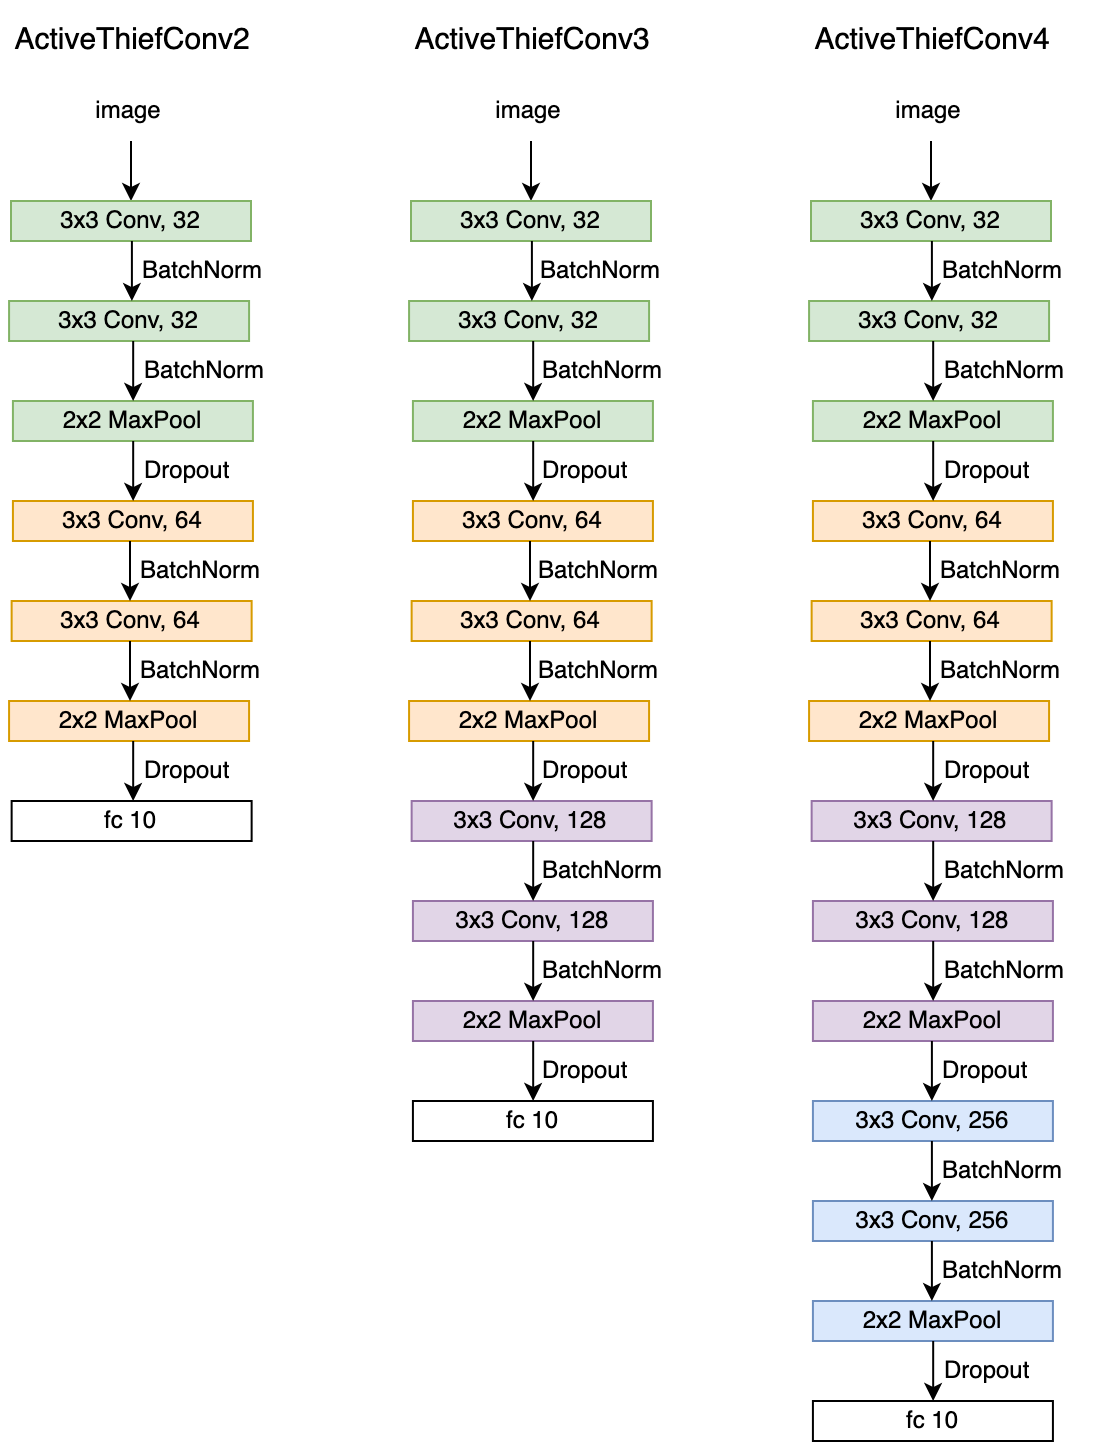
\includegraphics[width=\linewidth]{images/ActiveThiefConvs.png}
    \caption[ActiveThiefConv Architectures]{Example Network Architectures for CIFAR-10.}
    \label{fig:ActiveThiefArchitectures}
\end{figure}



\section{Experimental Results}
\label{sec:Appendix:Results}
This section is intended to provide extended material to selected experiments in section \ref{sec:Evaluation:Results}. We especially
include additional plots for the Continual Active Learning experiments which we were not able to include in the main text due to
space constraints.

\subsection{Target and Substitute Model Comparison}
\label{sec:Appendix:TargetSubstituteComparison}
Here we include the progression of Model Agreement for the experiments conducted in section \ref{sec:Evaluation:Results:MS:ActiveThief}.

\begin{figure}[!htb]
    \centering
    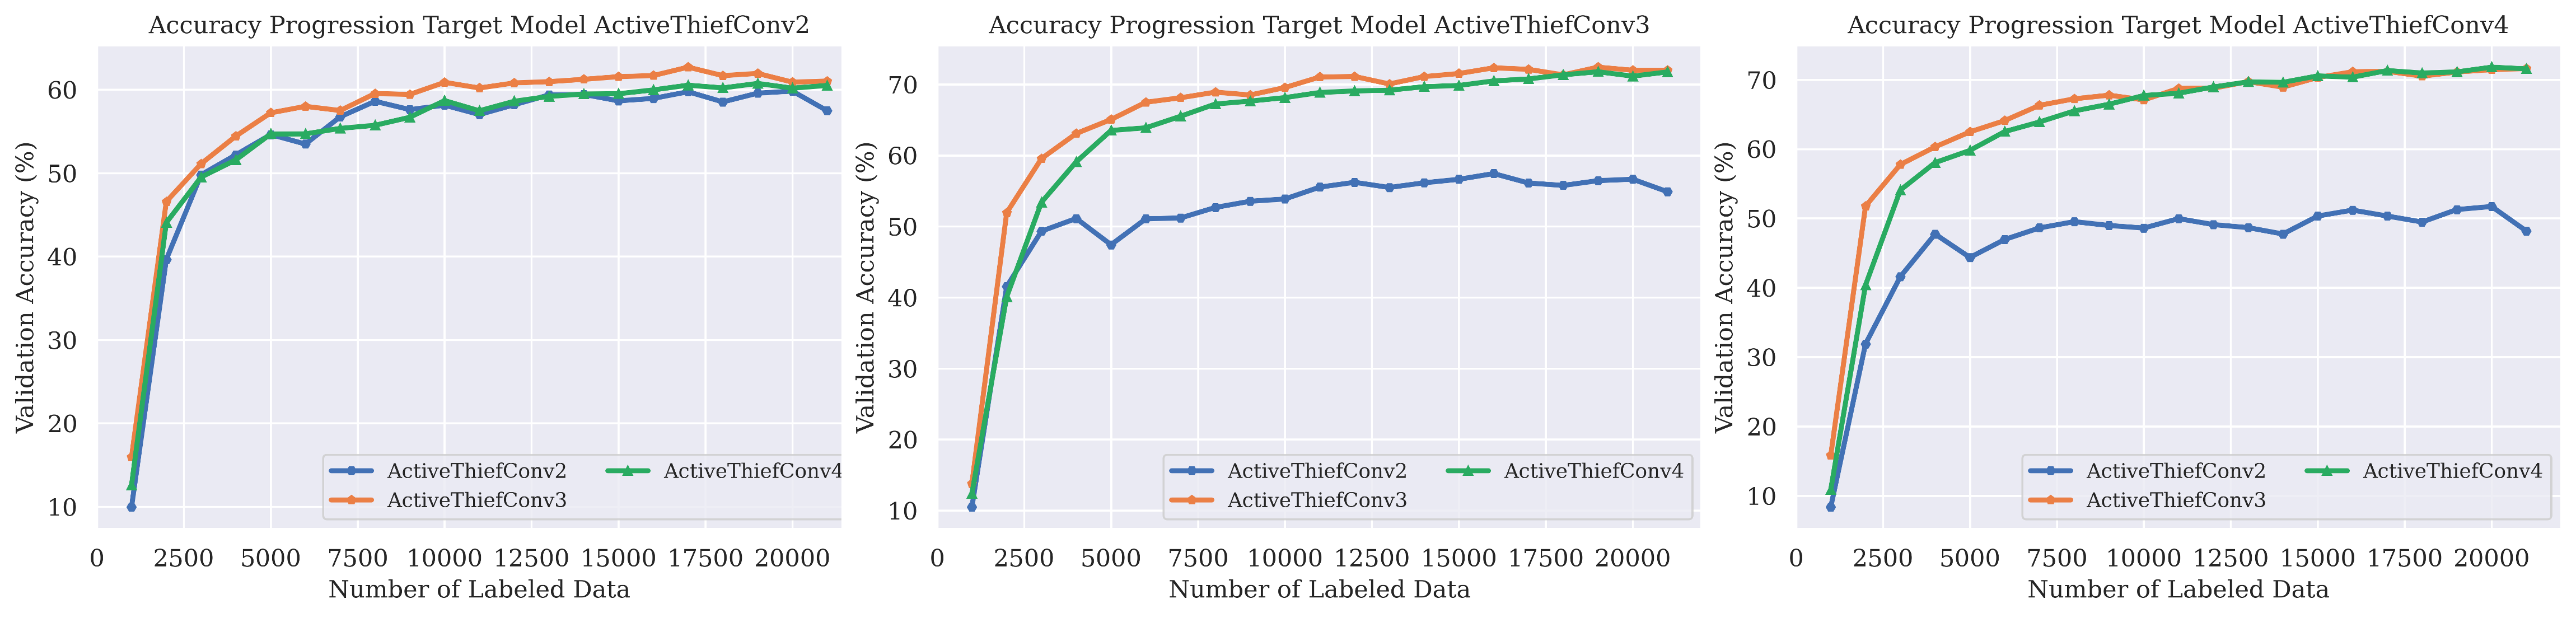
\includegraphics[width=\linewidth]{images/results_CALMS/cifar10_model_comp.png}
    \caption{Agreement Progression for Model Stealing on CIFAR-10 using different ActiveThief models}
    \label{fig:CIFAR10modelComp}
\end{figure}

\begin{figure}[!htb]
    \centering
    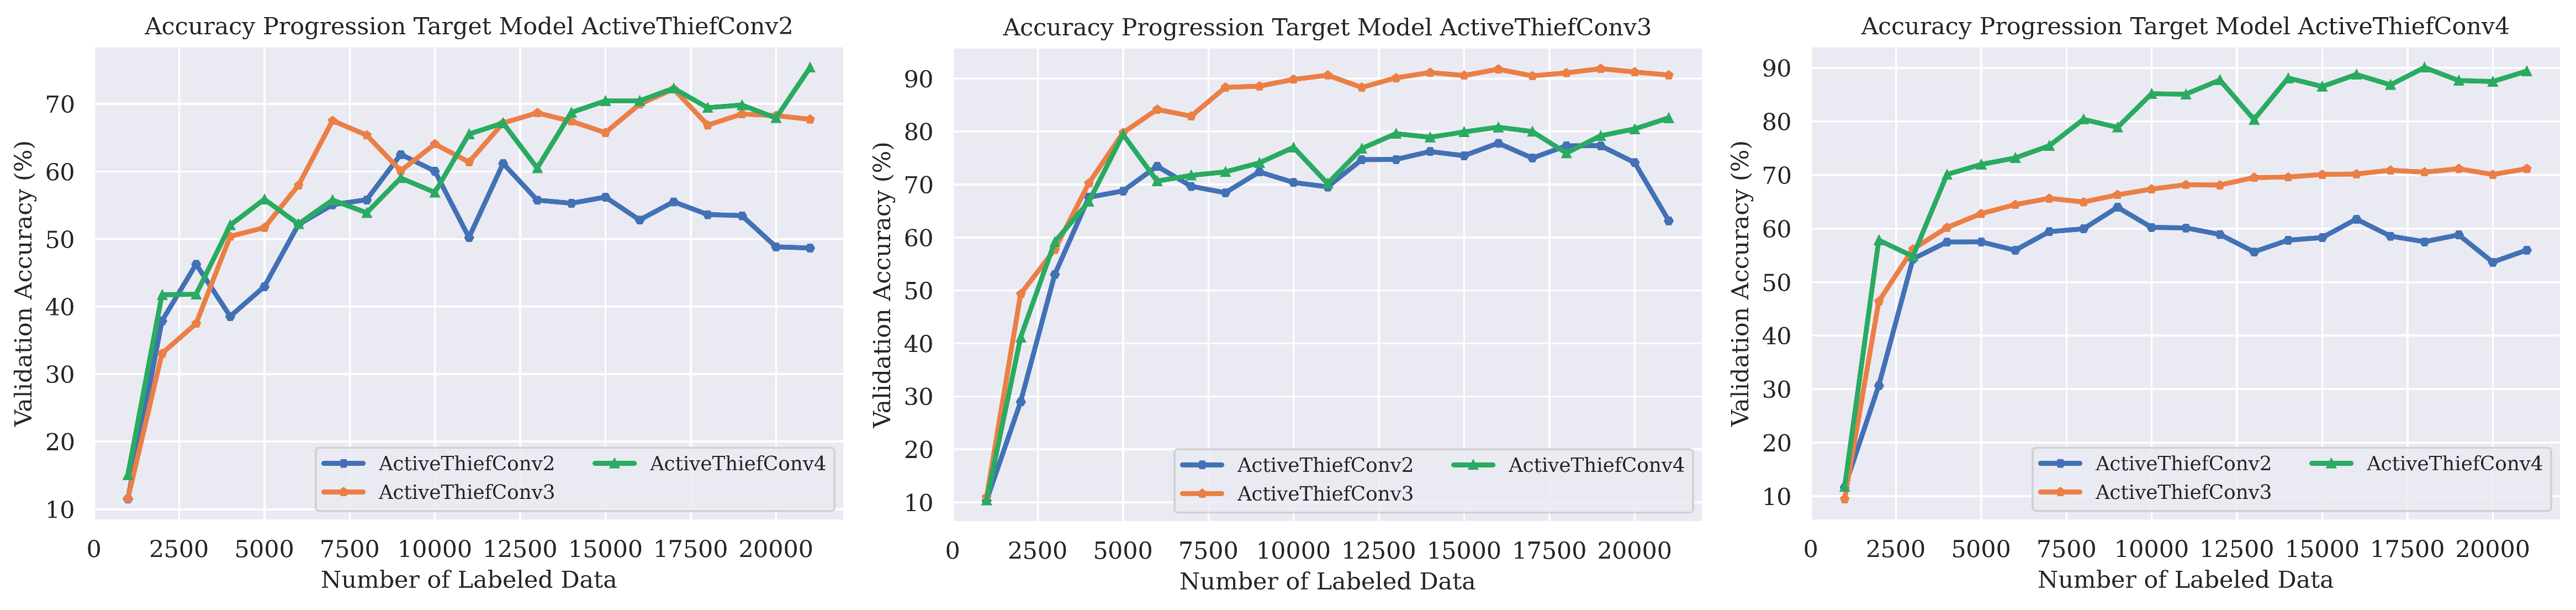
\includegraphics[width=\linewidth]{images/results_CALMS/mnist_model_comp.png}
    \caption{Agreement Progression for Model Stealing on MNIST using different ActiveThief models}
    \label{fig:MNISTmodelComp}
\end{figure}


\subsection{Continual Active Learning for Model Stealing}
\label{sec:Appendix:CALMS}
This section contains plots of the full runs of all experiments in section \ref{sec:Evaluation:Results:MS:CAL}.

\subsubsection{MNIST}
\label{sec:Appendix:CALMS:MNIST}
In this section, we present the full runs of all experiments which involve Continual Active Learning using MNIST as a Target Model Dataset.


\begin{figure}[!htb]
    \centering
    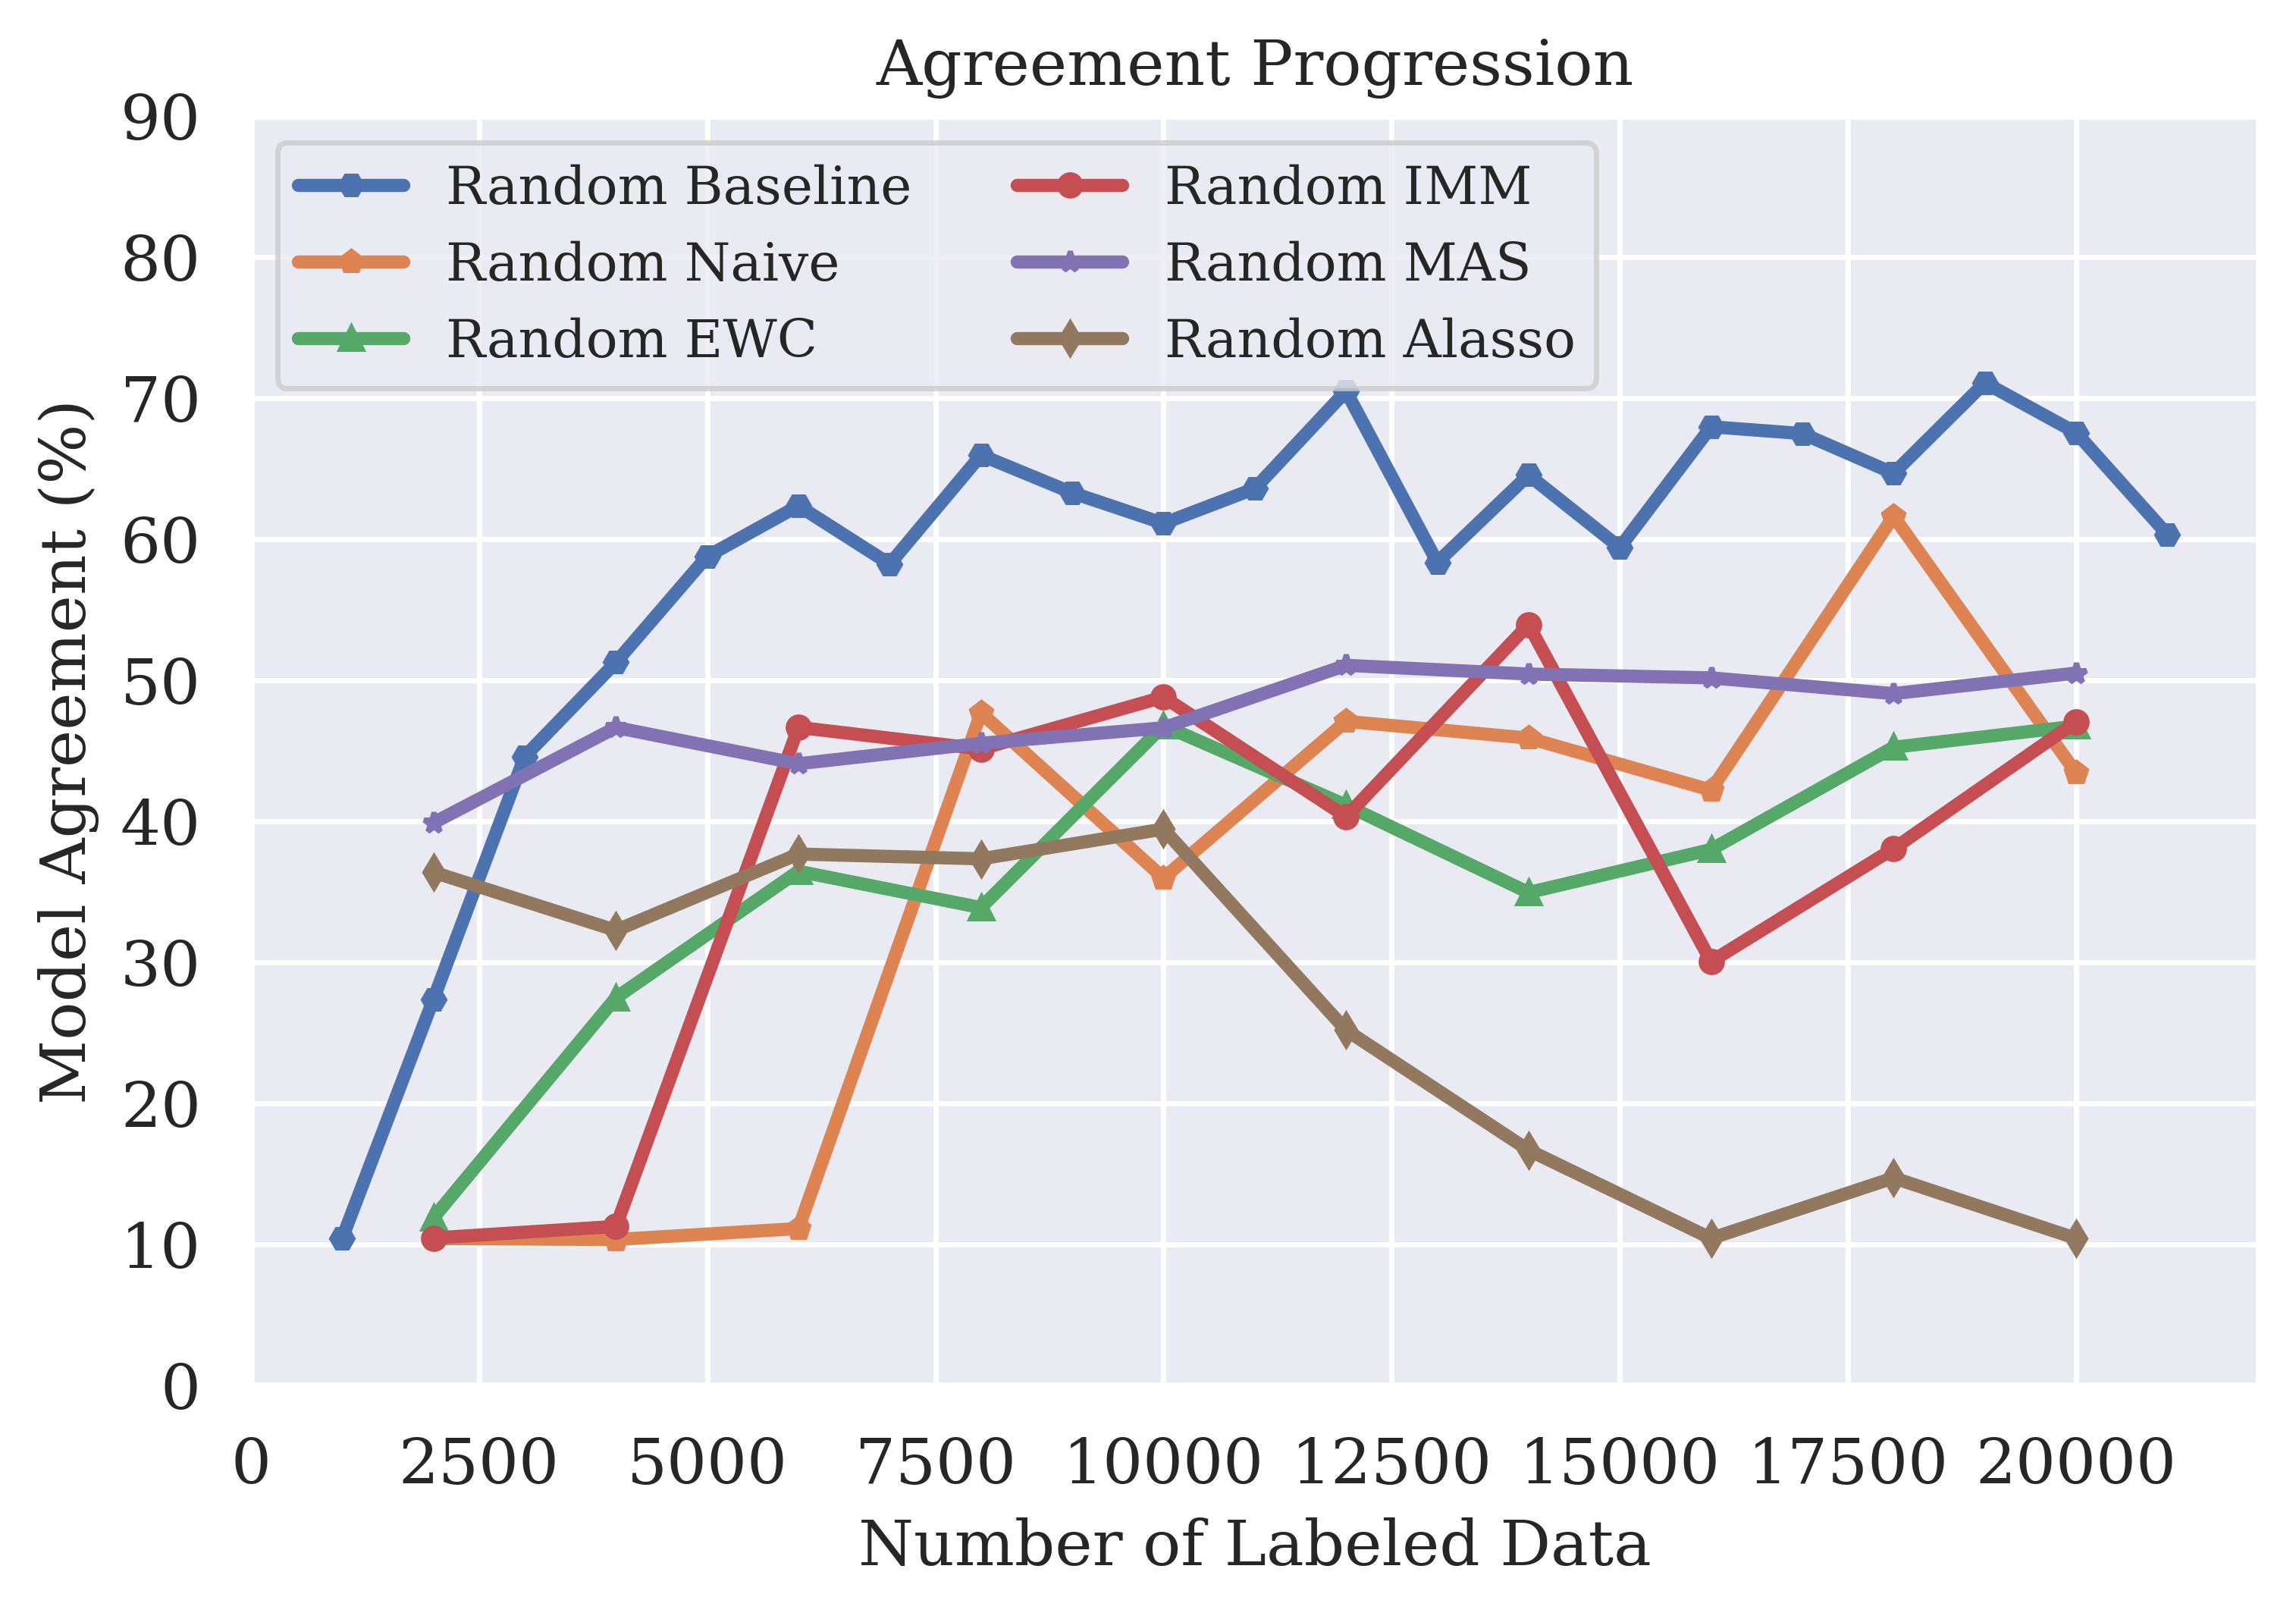
\includegraphics[width=0.5\linewidth]{images/results_CALMS/mnist_label_random.png}
    \caption{Agreement Comparison for Model Stealing on MNIST using the predicted class label and the Active Learning strategy Random}
    \label{fig:CALMSMNISTLabelRandom}
\end{figure}

\begin{figure}[!htb]
    \centering
    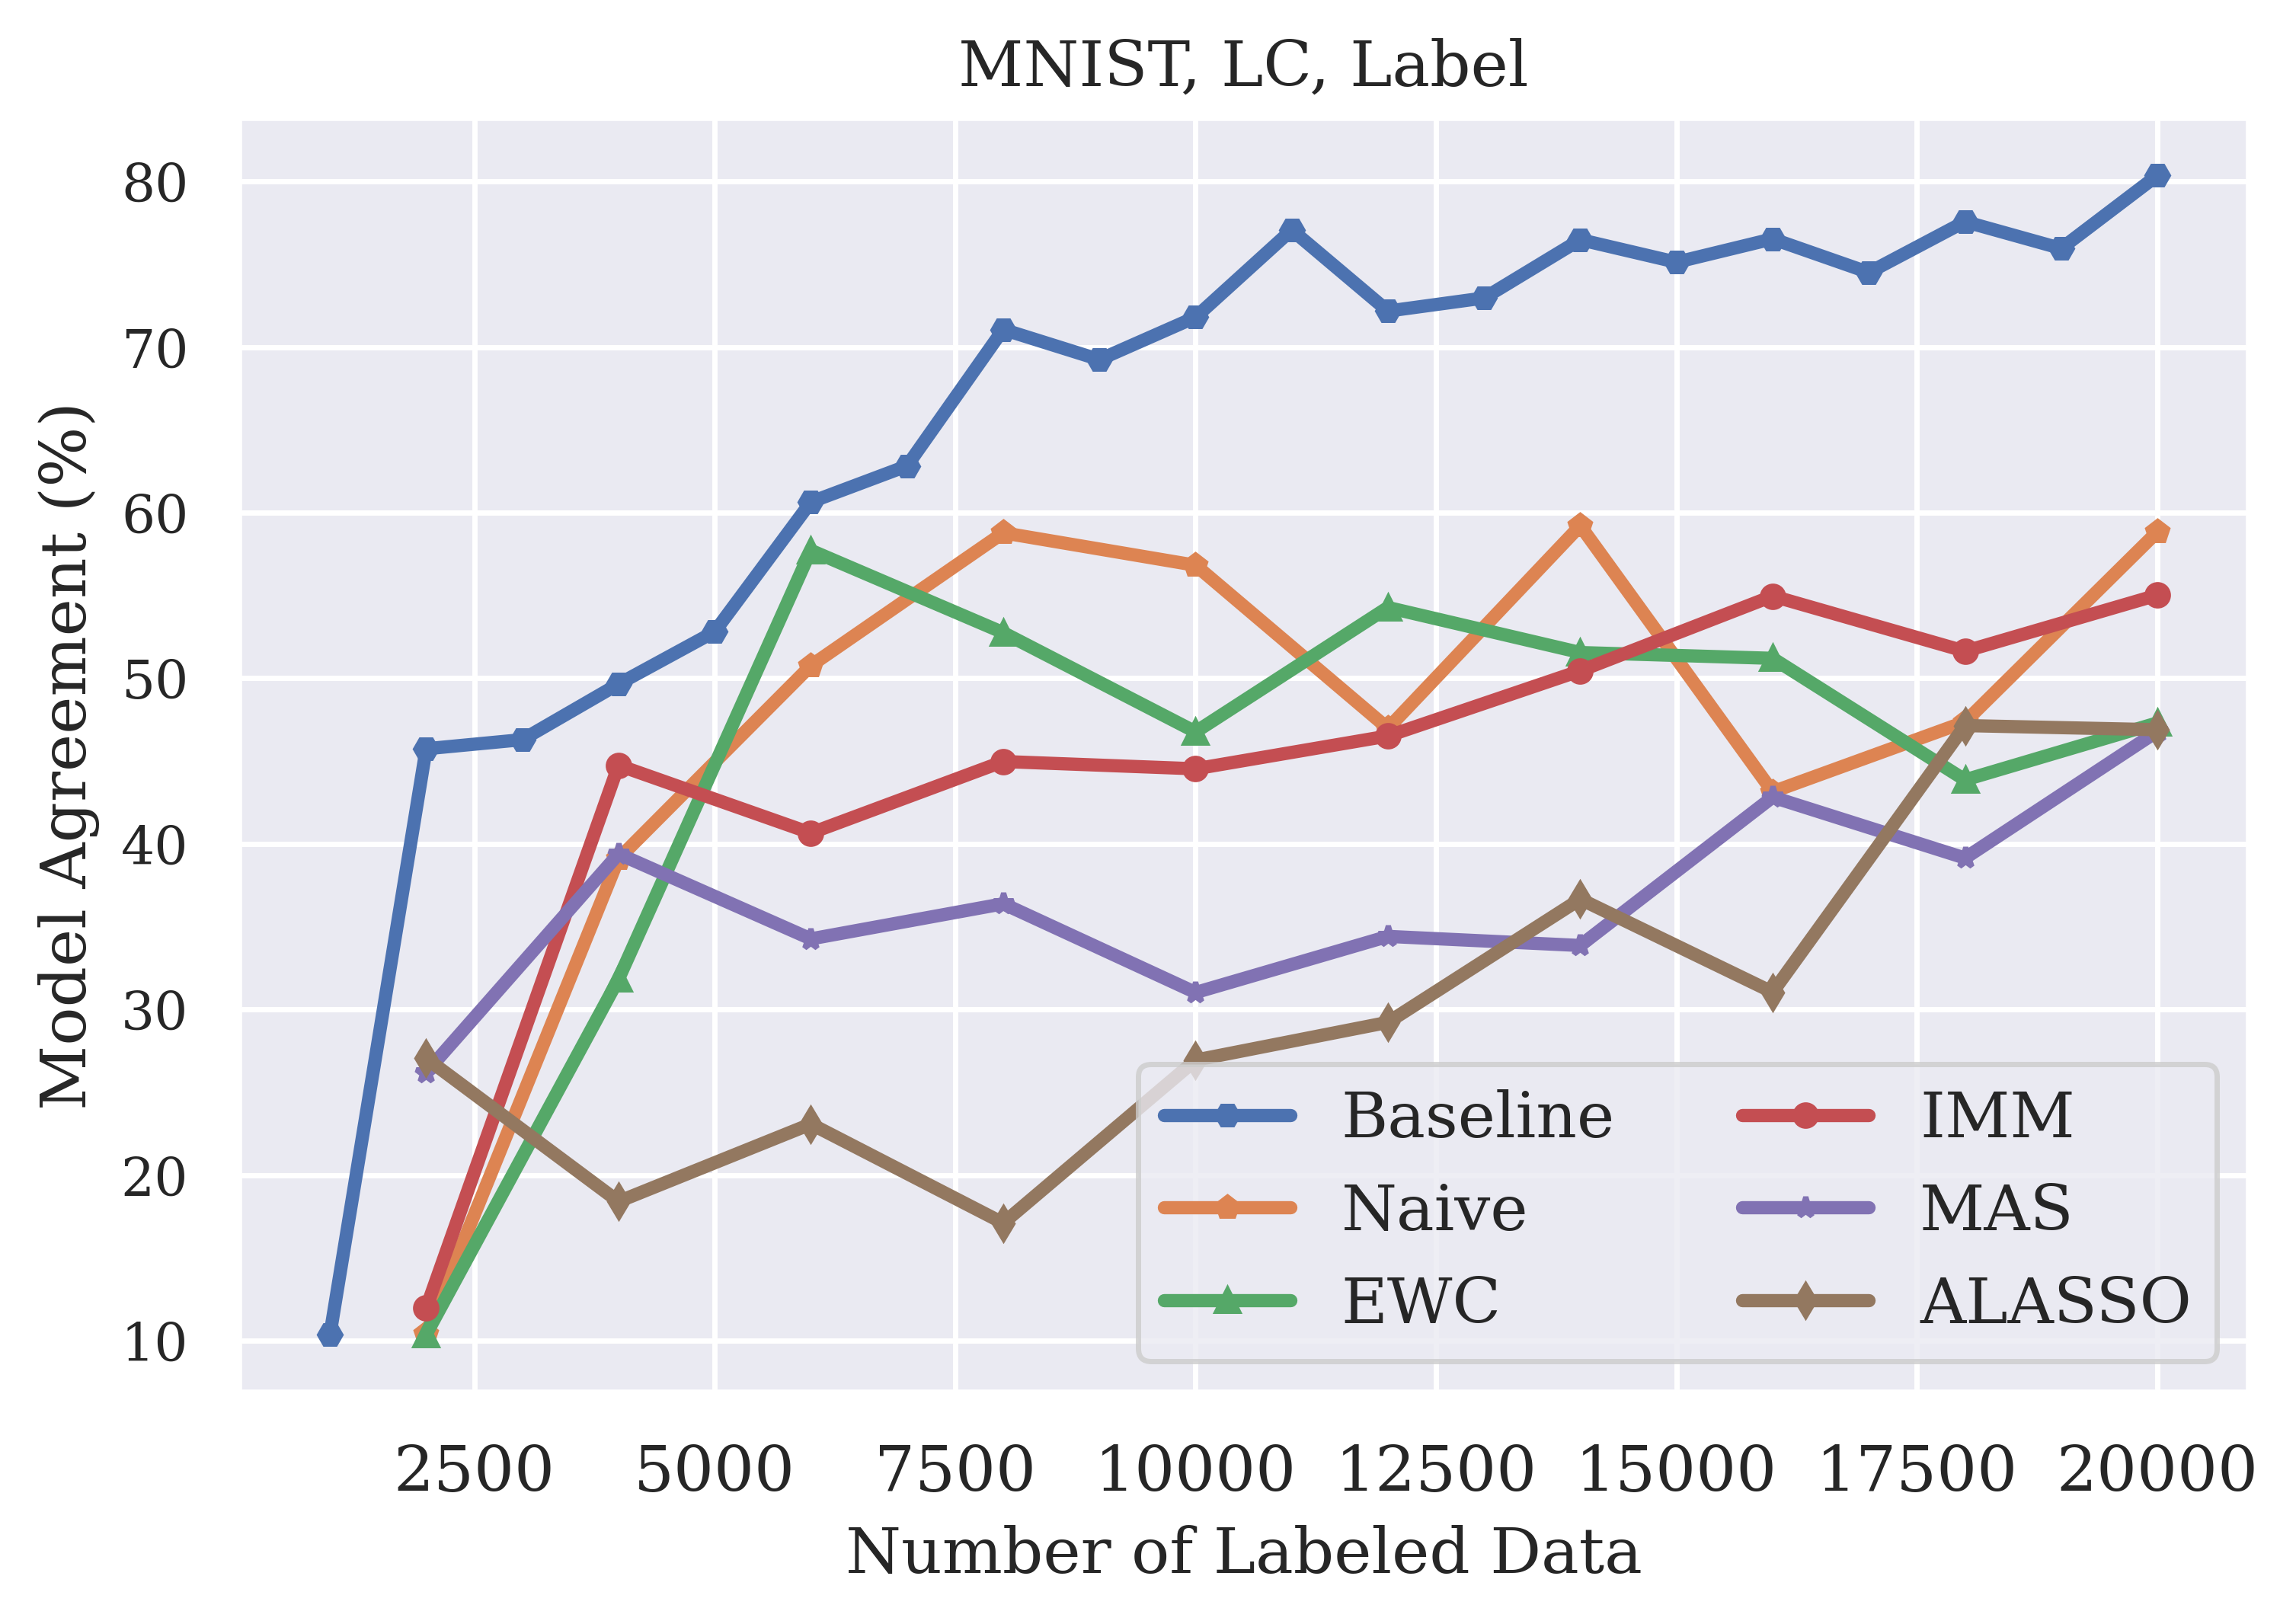
\includegraphics[width=0.5\linewidth]{images/results_CALMS/mnist_label_lc.png}
    \caption{Agreement Comparison for Model Stealing on MNIST using the predicted class label and the Active Learning strategy \gls{lc}}
    \label{fig:CALMSMNISTLabelLC}
\end{figure}

\begin{figure}[!htb]
    \centering
    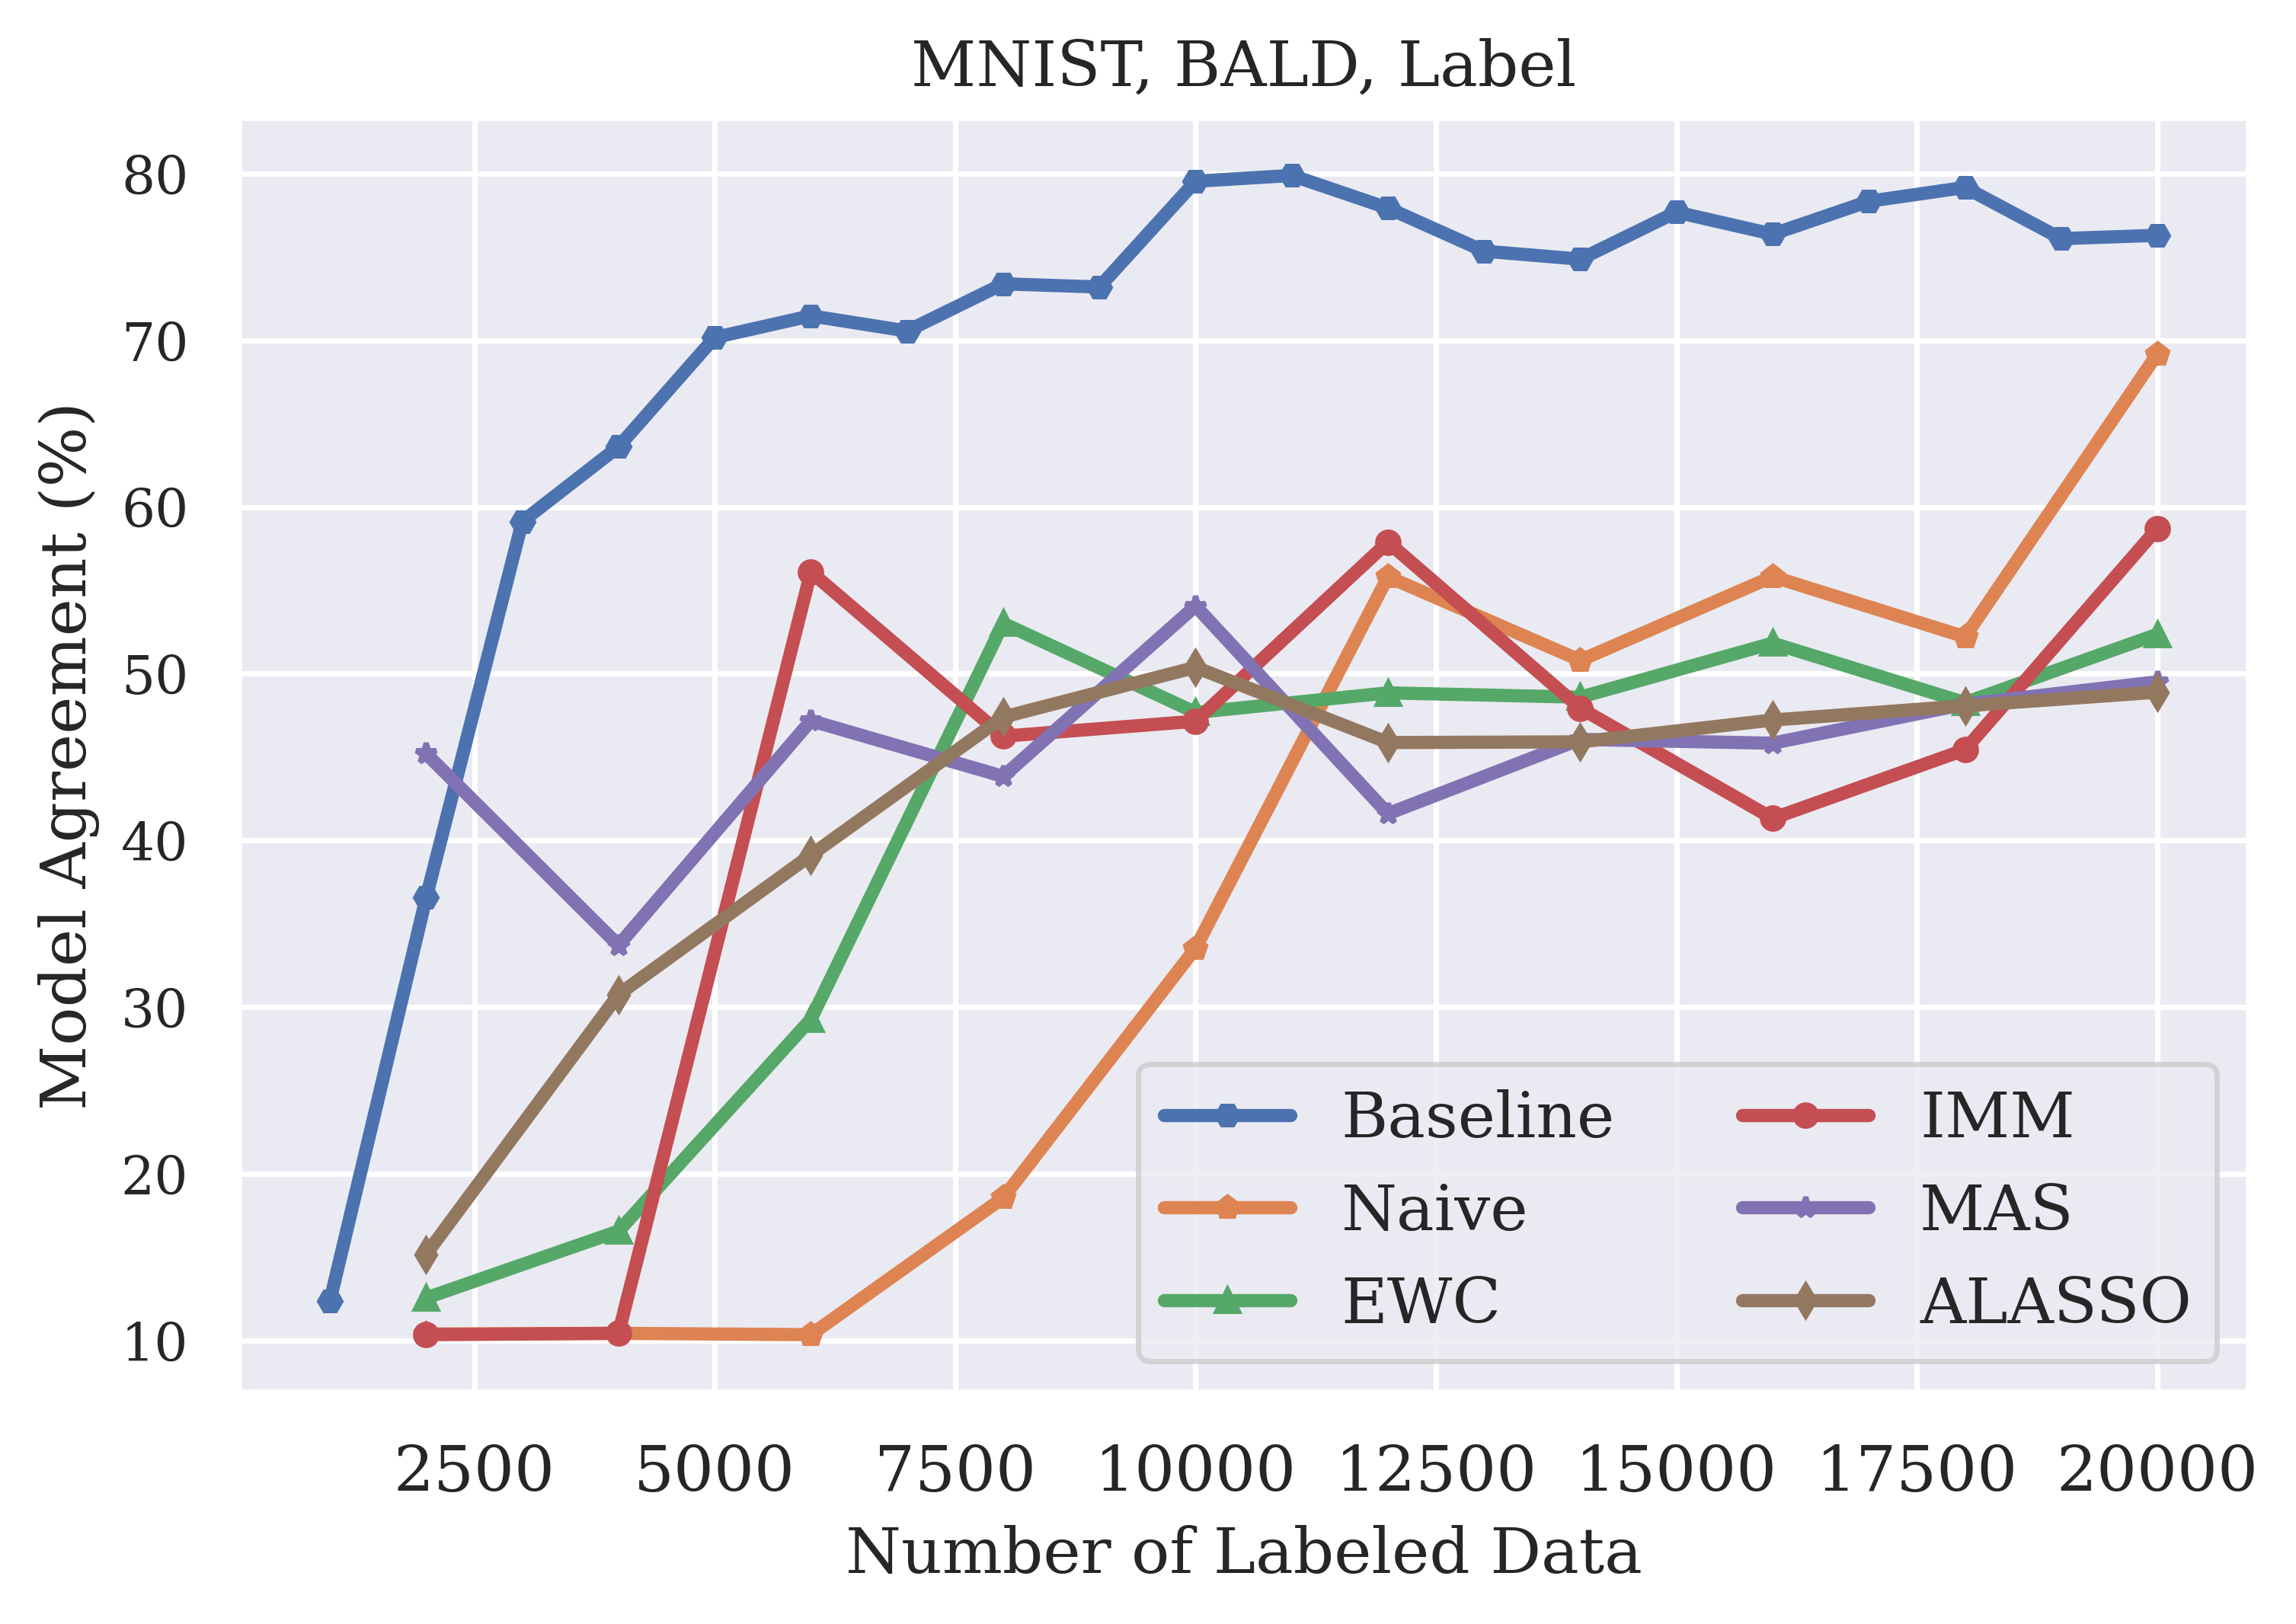
\includegraphics[width=0.5\linewidth]{images/results_CALMS/mnist_label_bald.png}
    \caption{Accuracy Comparison for Model Stealing on MNIST using the predicted class label and the Active Learning strategy \gls{bald}}
    \label{fig:CALMSMNISTLabelBALD}
\end{figure}

\begin{figure}[!htb]
    \centering
    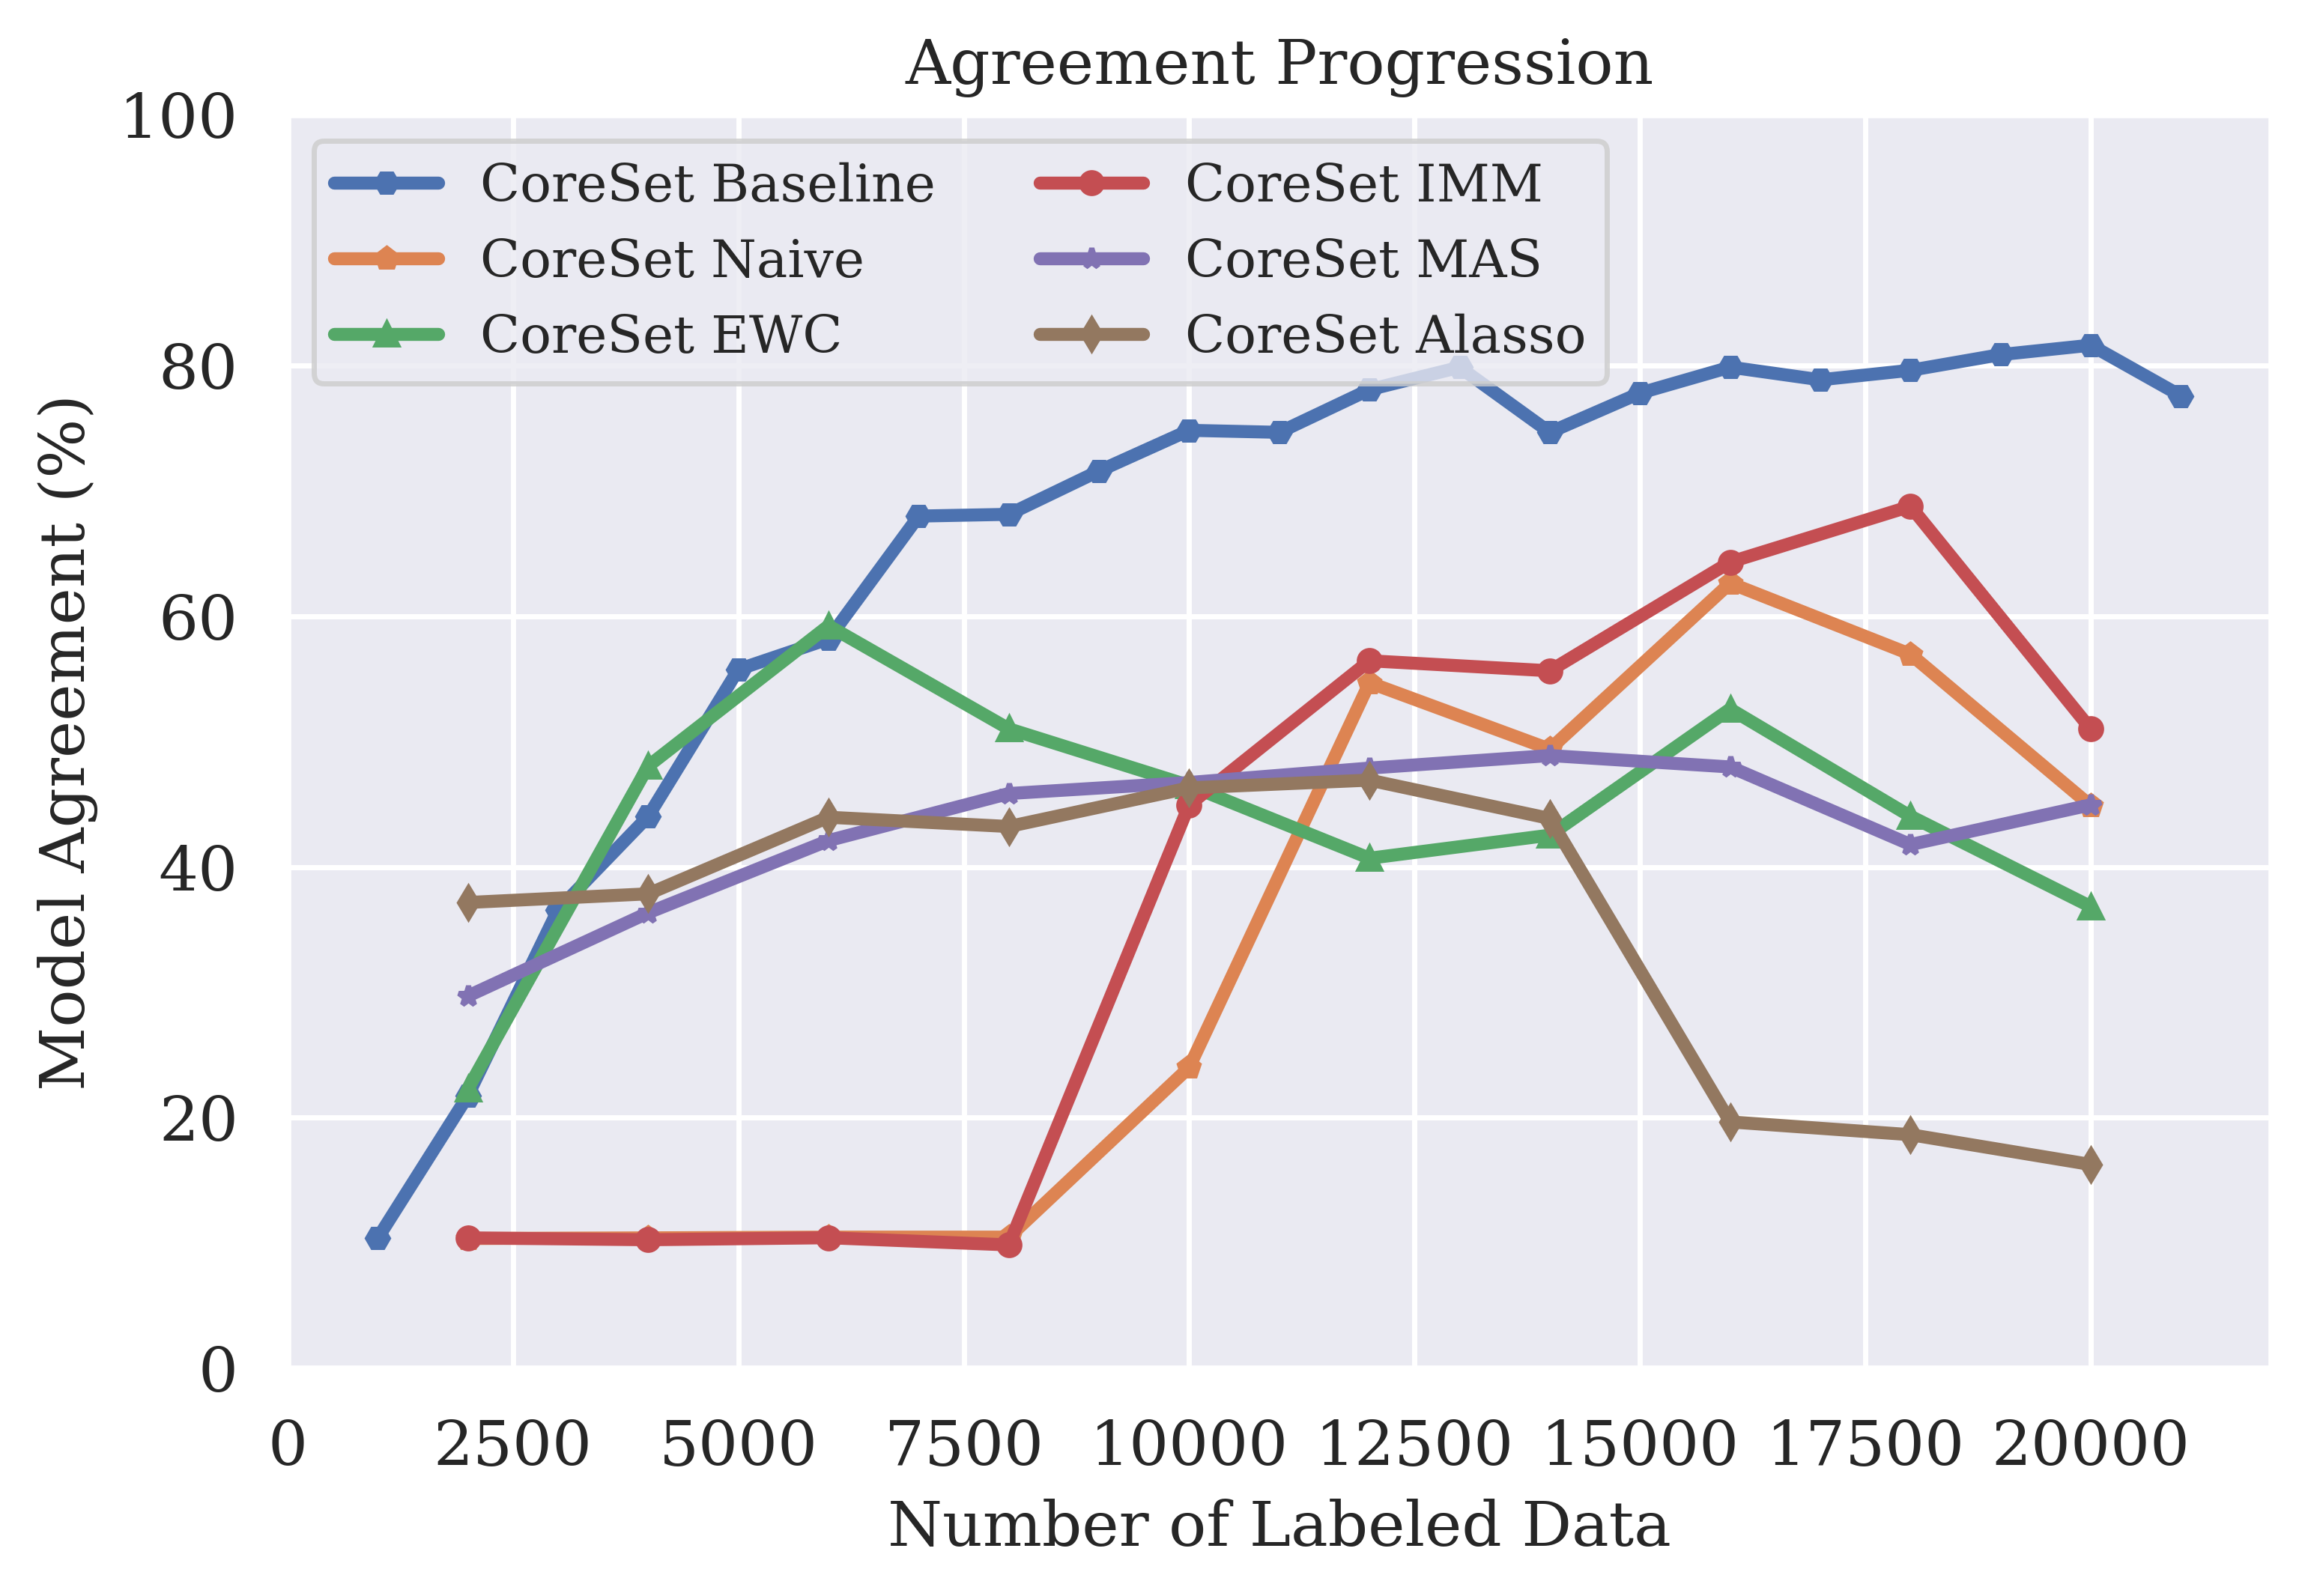
\includegraphics[width=0.5\linewidth]{images/results_CALMS/mnist_label_coreset.png}
    \caption{Agreement Comparison for Model Stealing on MNIST using the predicted class label and the Active Learning strategy CoreSet}
    \label{fig:CALMSMNISTLabelCoreSet}
\end{figure}

\begin{figure}[!htb]
    \centering
    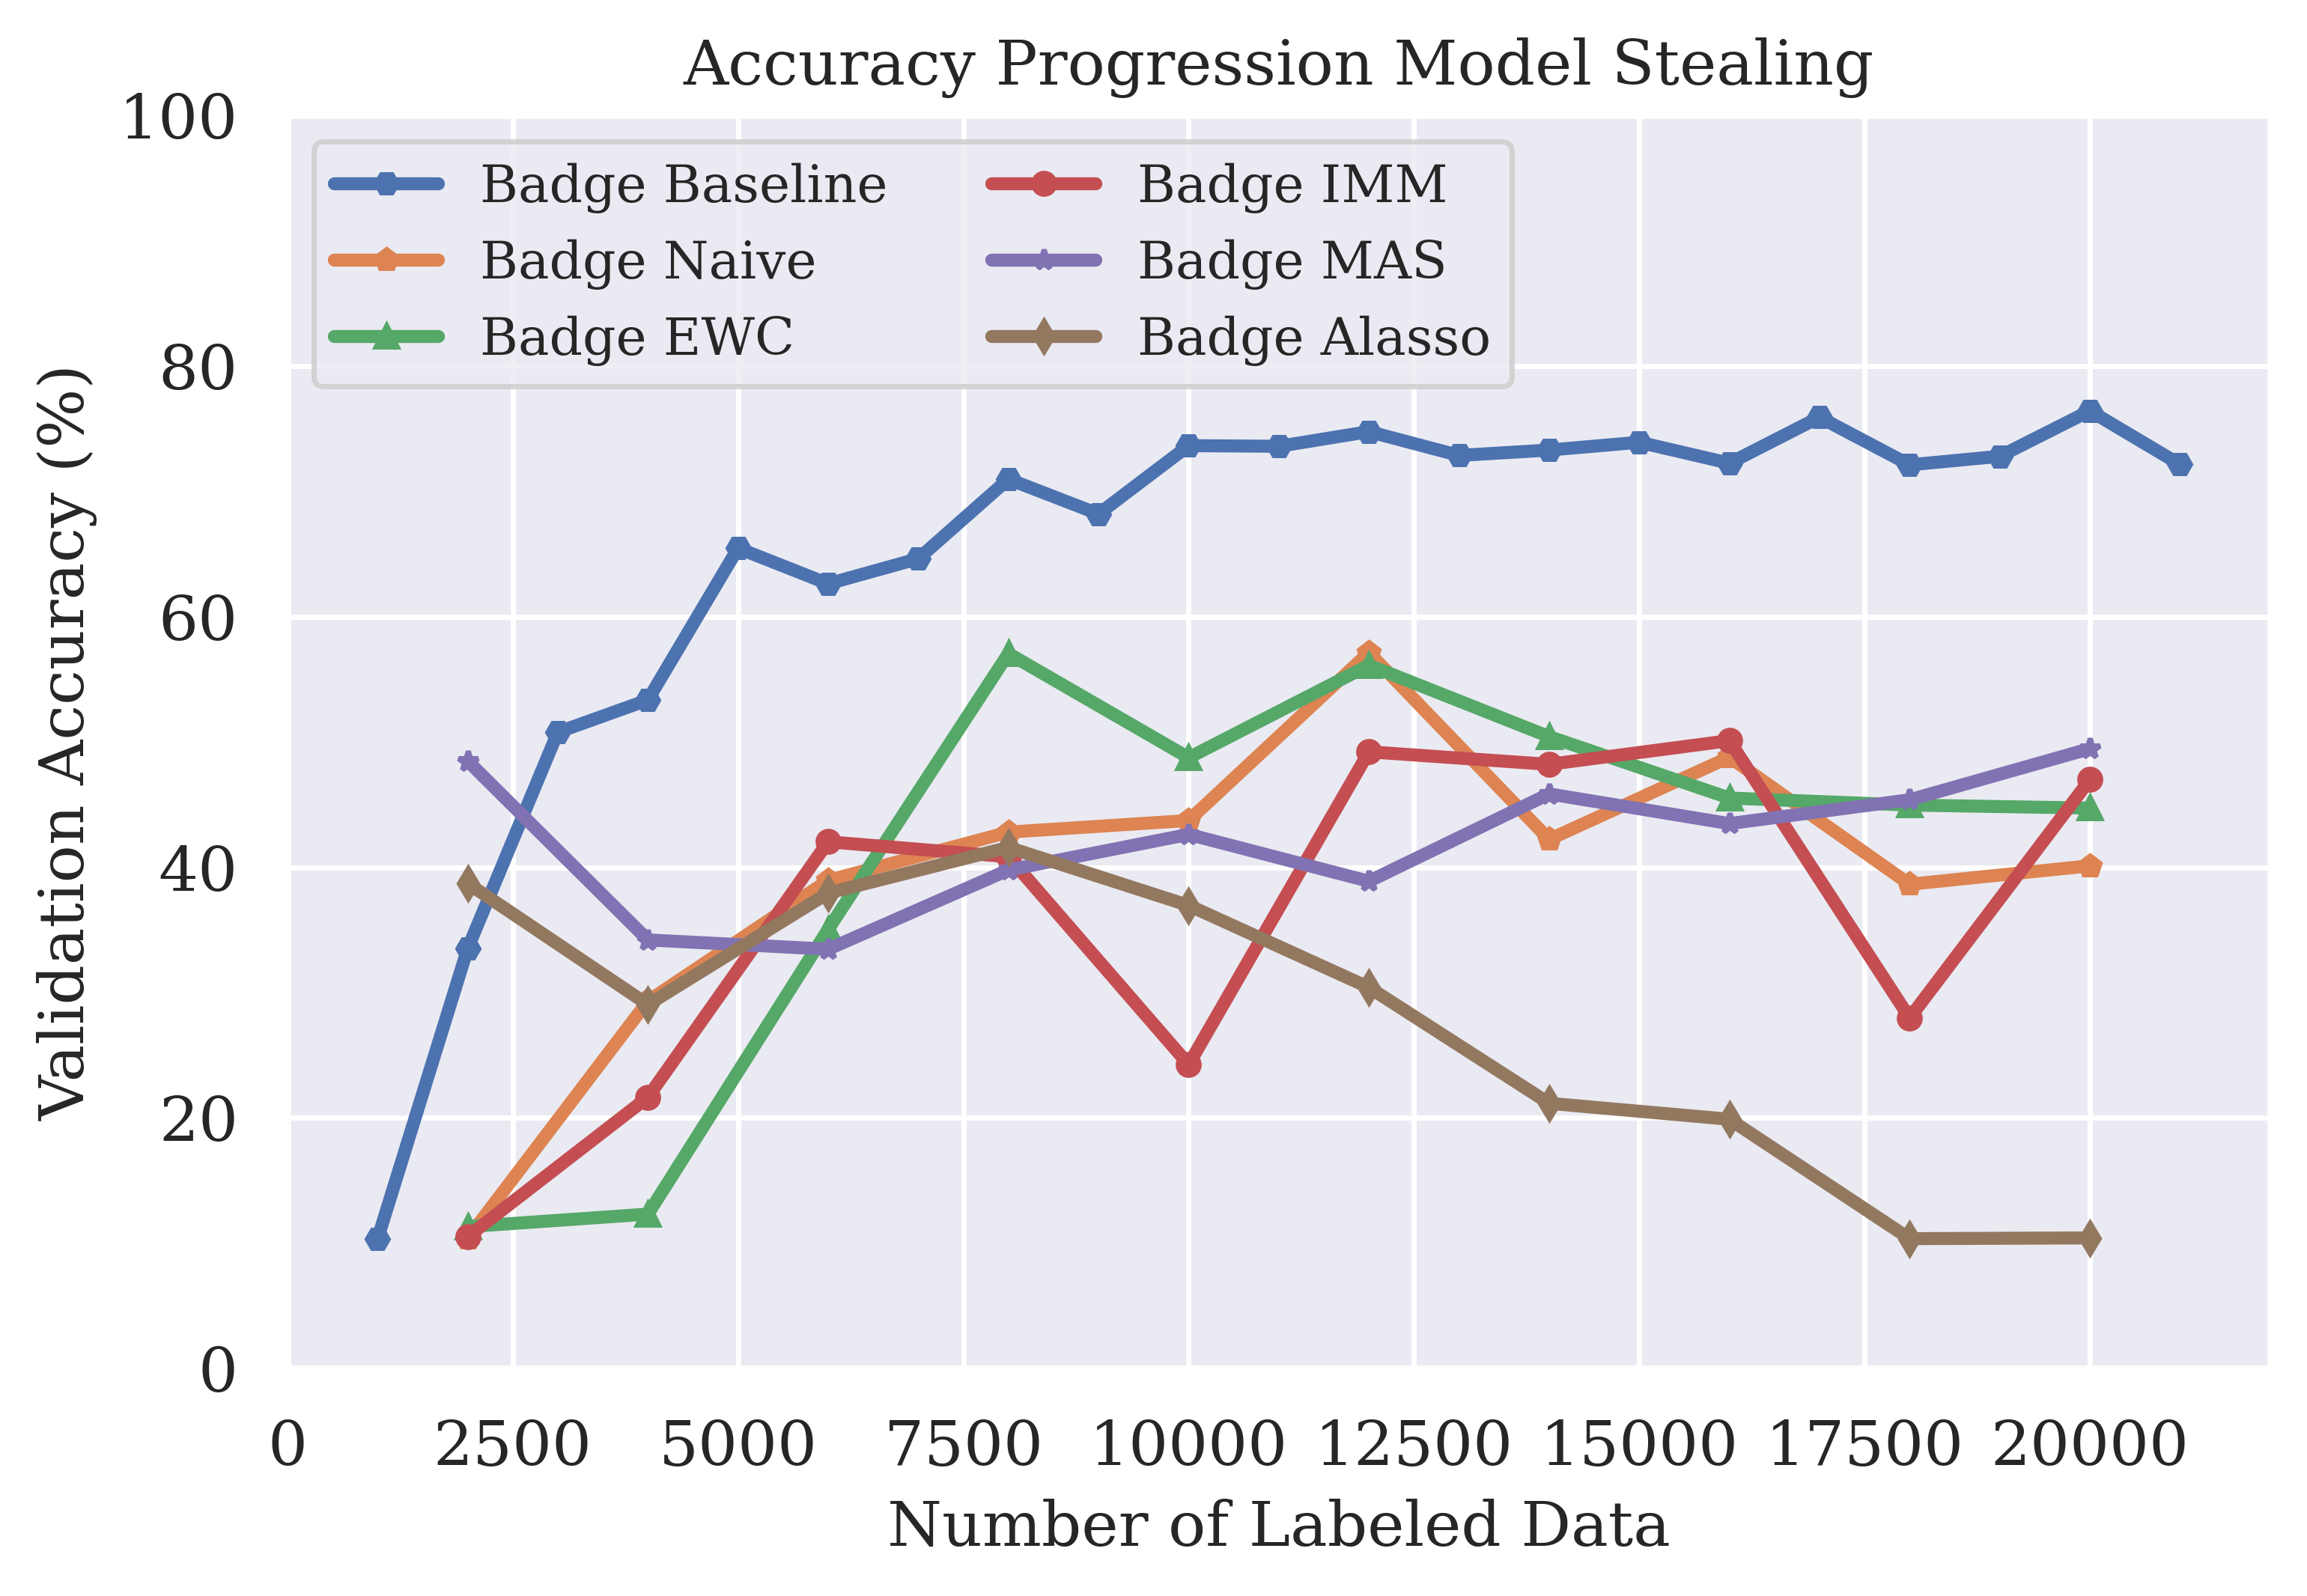
\includegraphics[width=0.5\linewidth]{images/results_CALMS/mnist_label_badge.png}
    \caption{Agreement Comparison for Model Stealing on MNIST using the predicted class label and the Active Learning strategy \gls{badge}}
    \label{fig:CALMSMNISTLabelBadge}
\end{figure}

%Softmax
\begin{figure}[!htb]
    \centering
    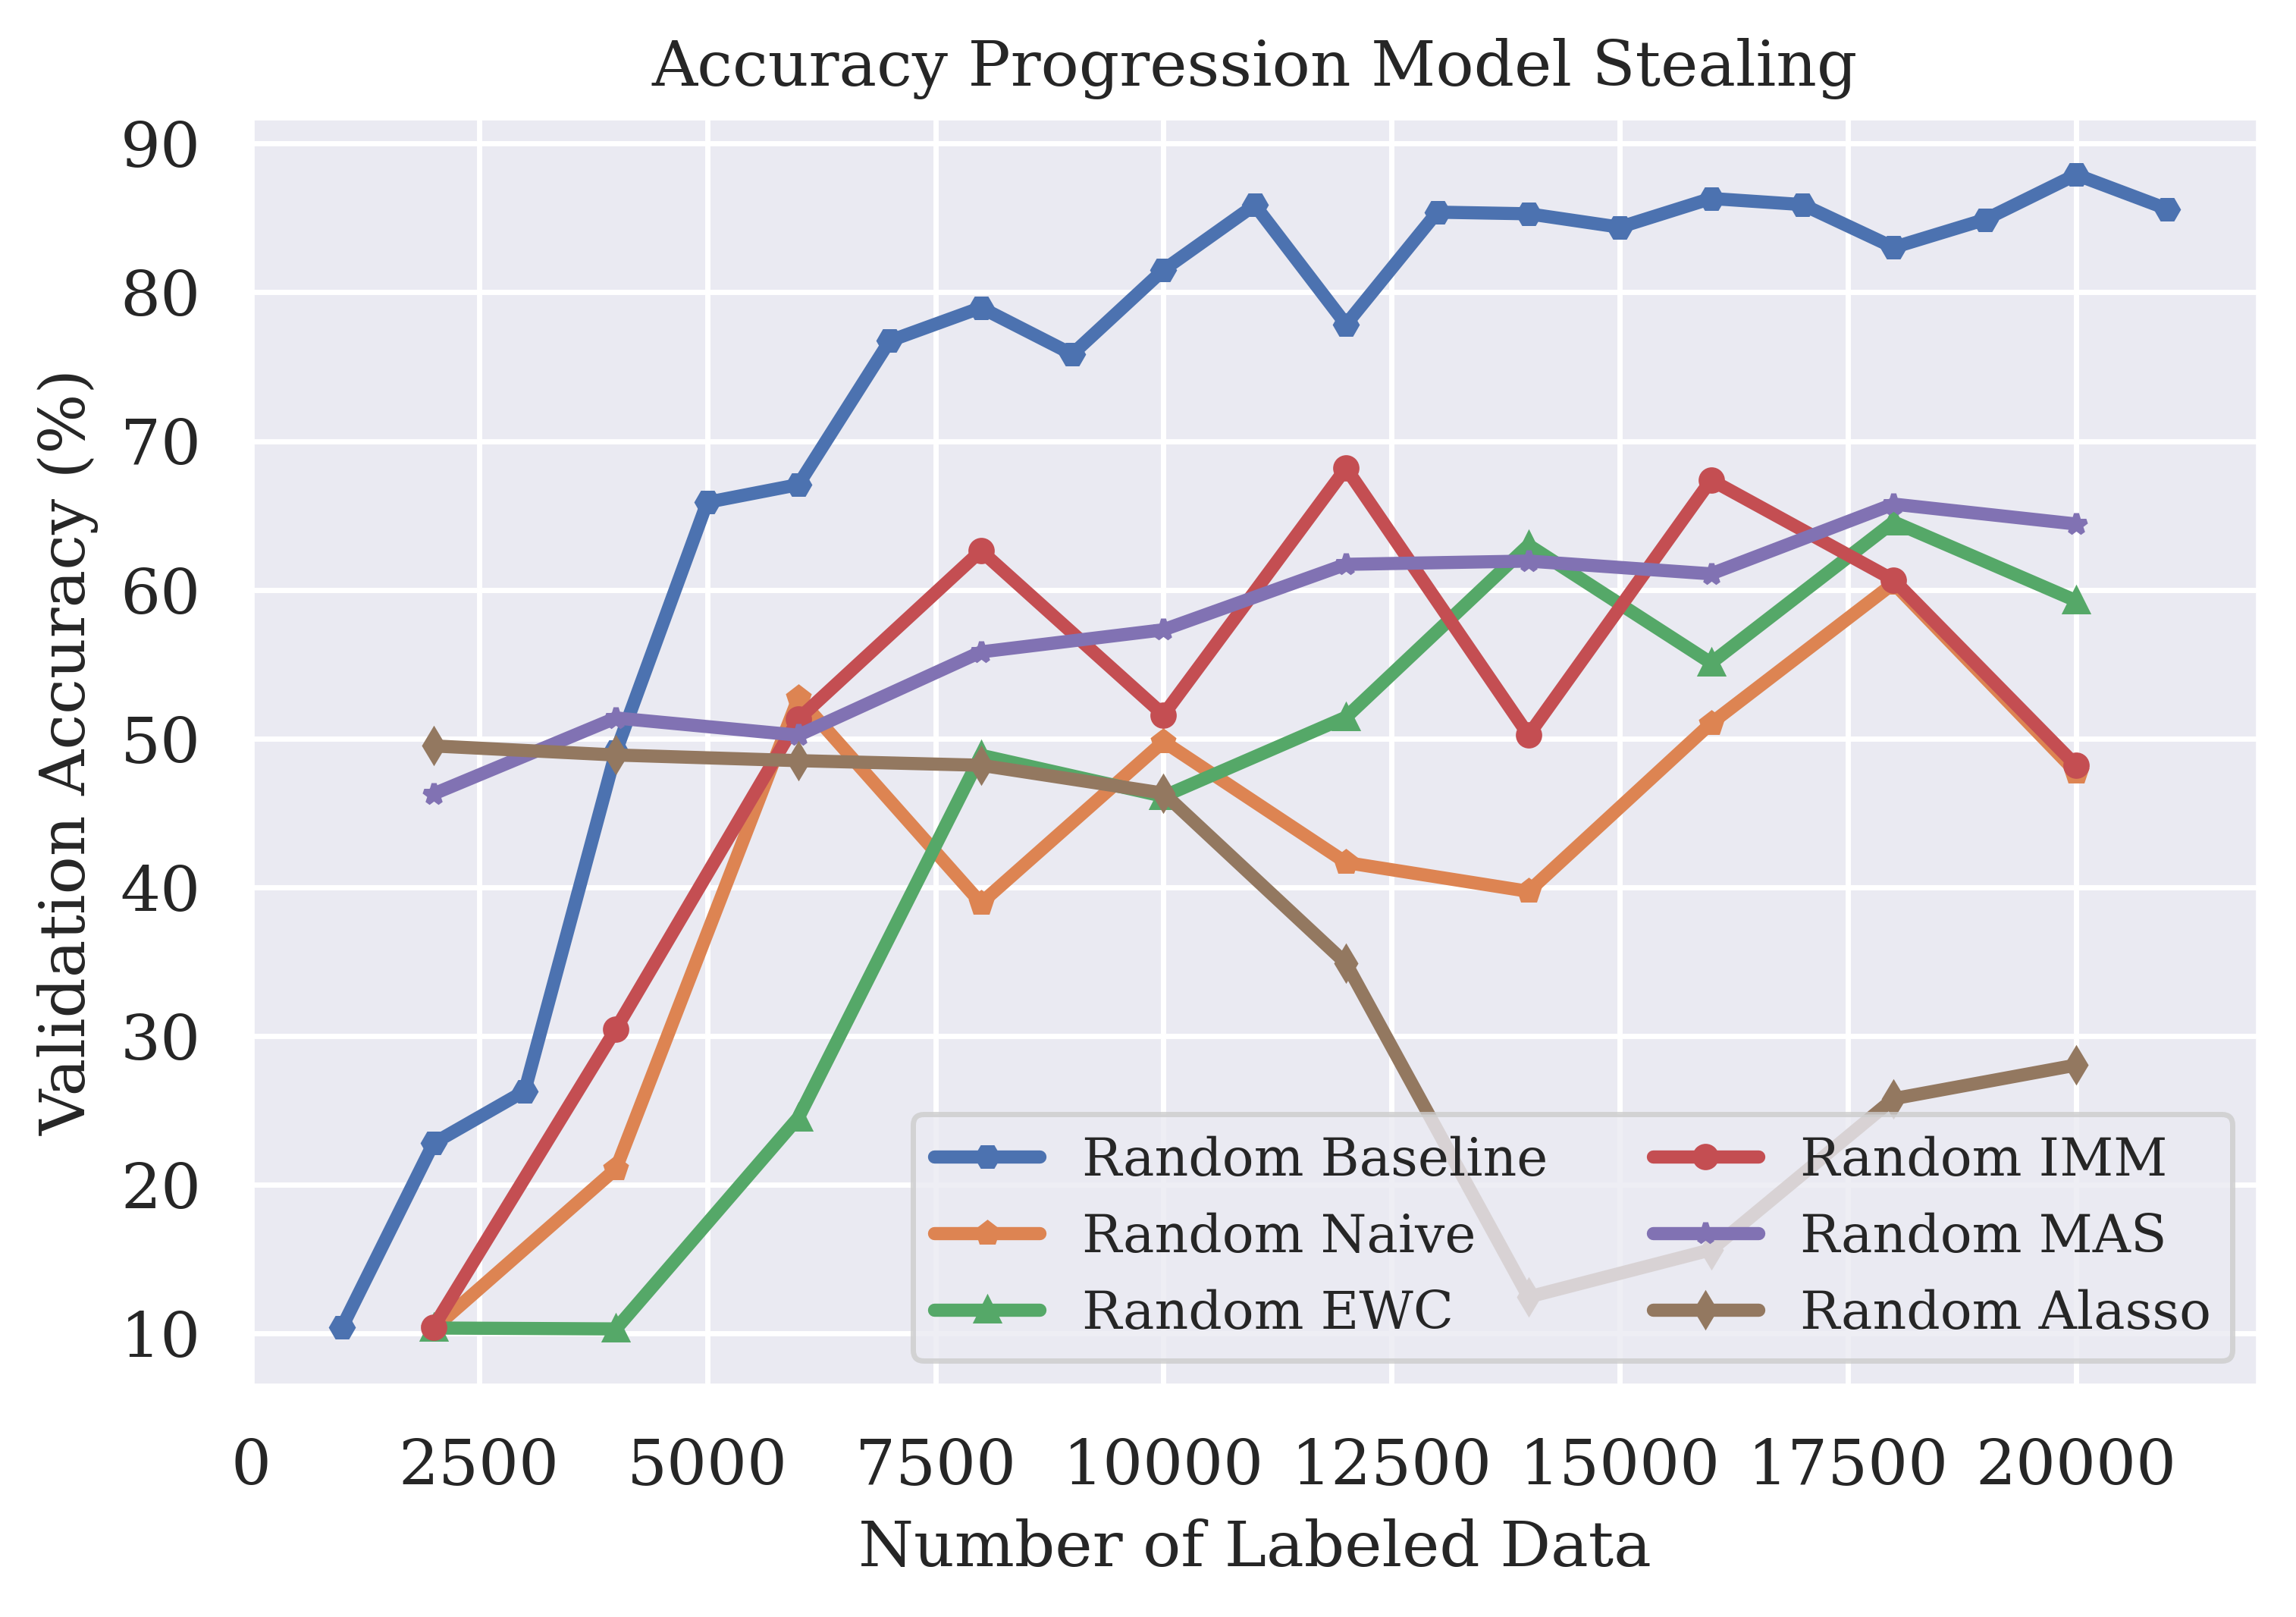
\includegraphics[width=0.5\linewidth]{images/results_CALMS/mnist_softmax_random.png}
    \caption{Agreement Comparison for Model Stealing on MNIST using the softmax output and the Active Learning strategy Random}
    \label{fig:CALMSMNISTSoftmaxRandom}
\end{figure}

\begin{figure}[!htb]
    \centering
    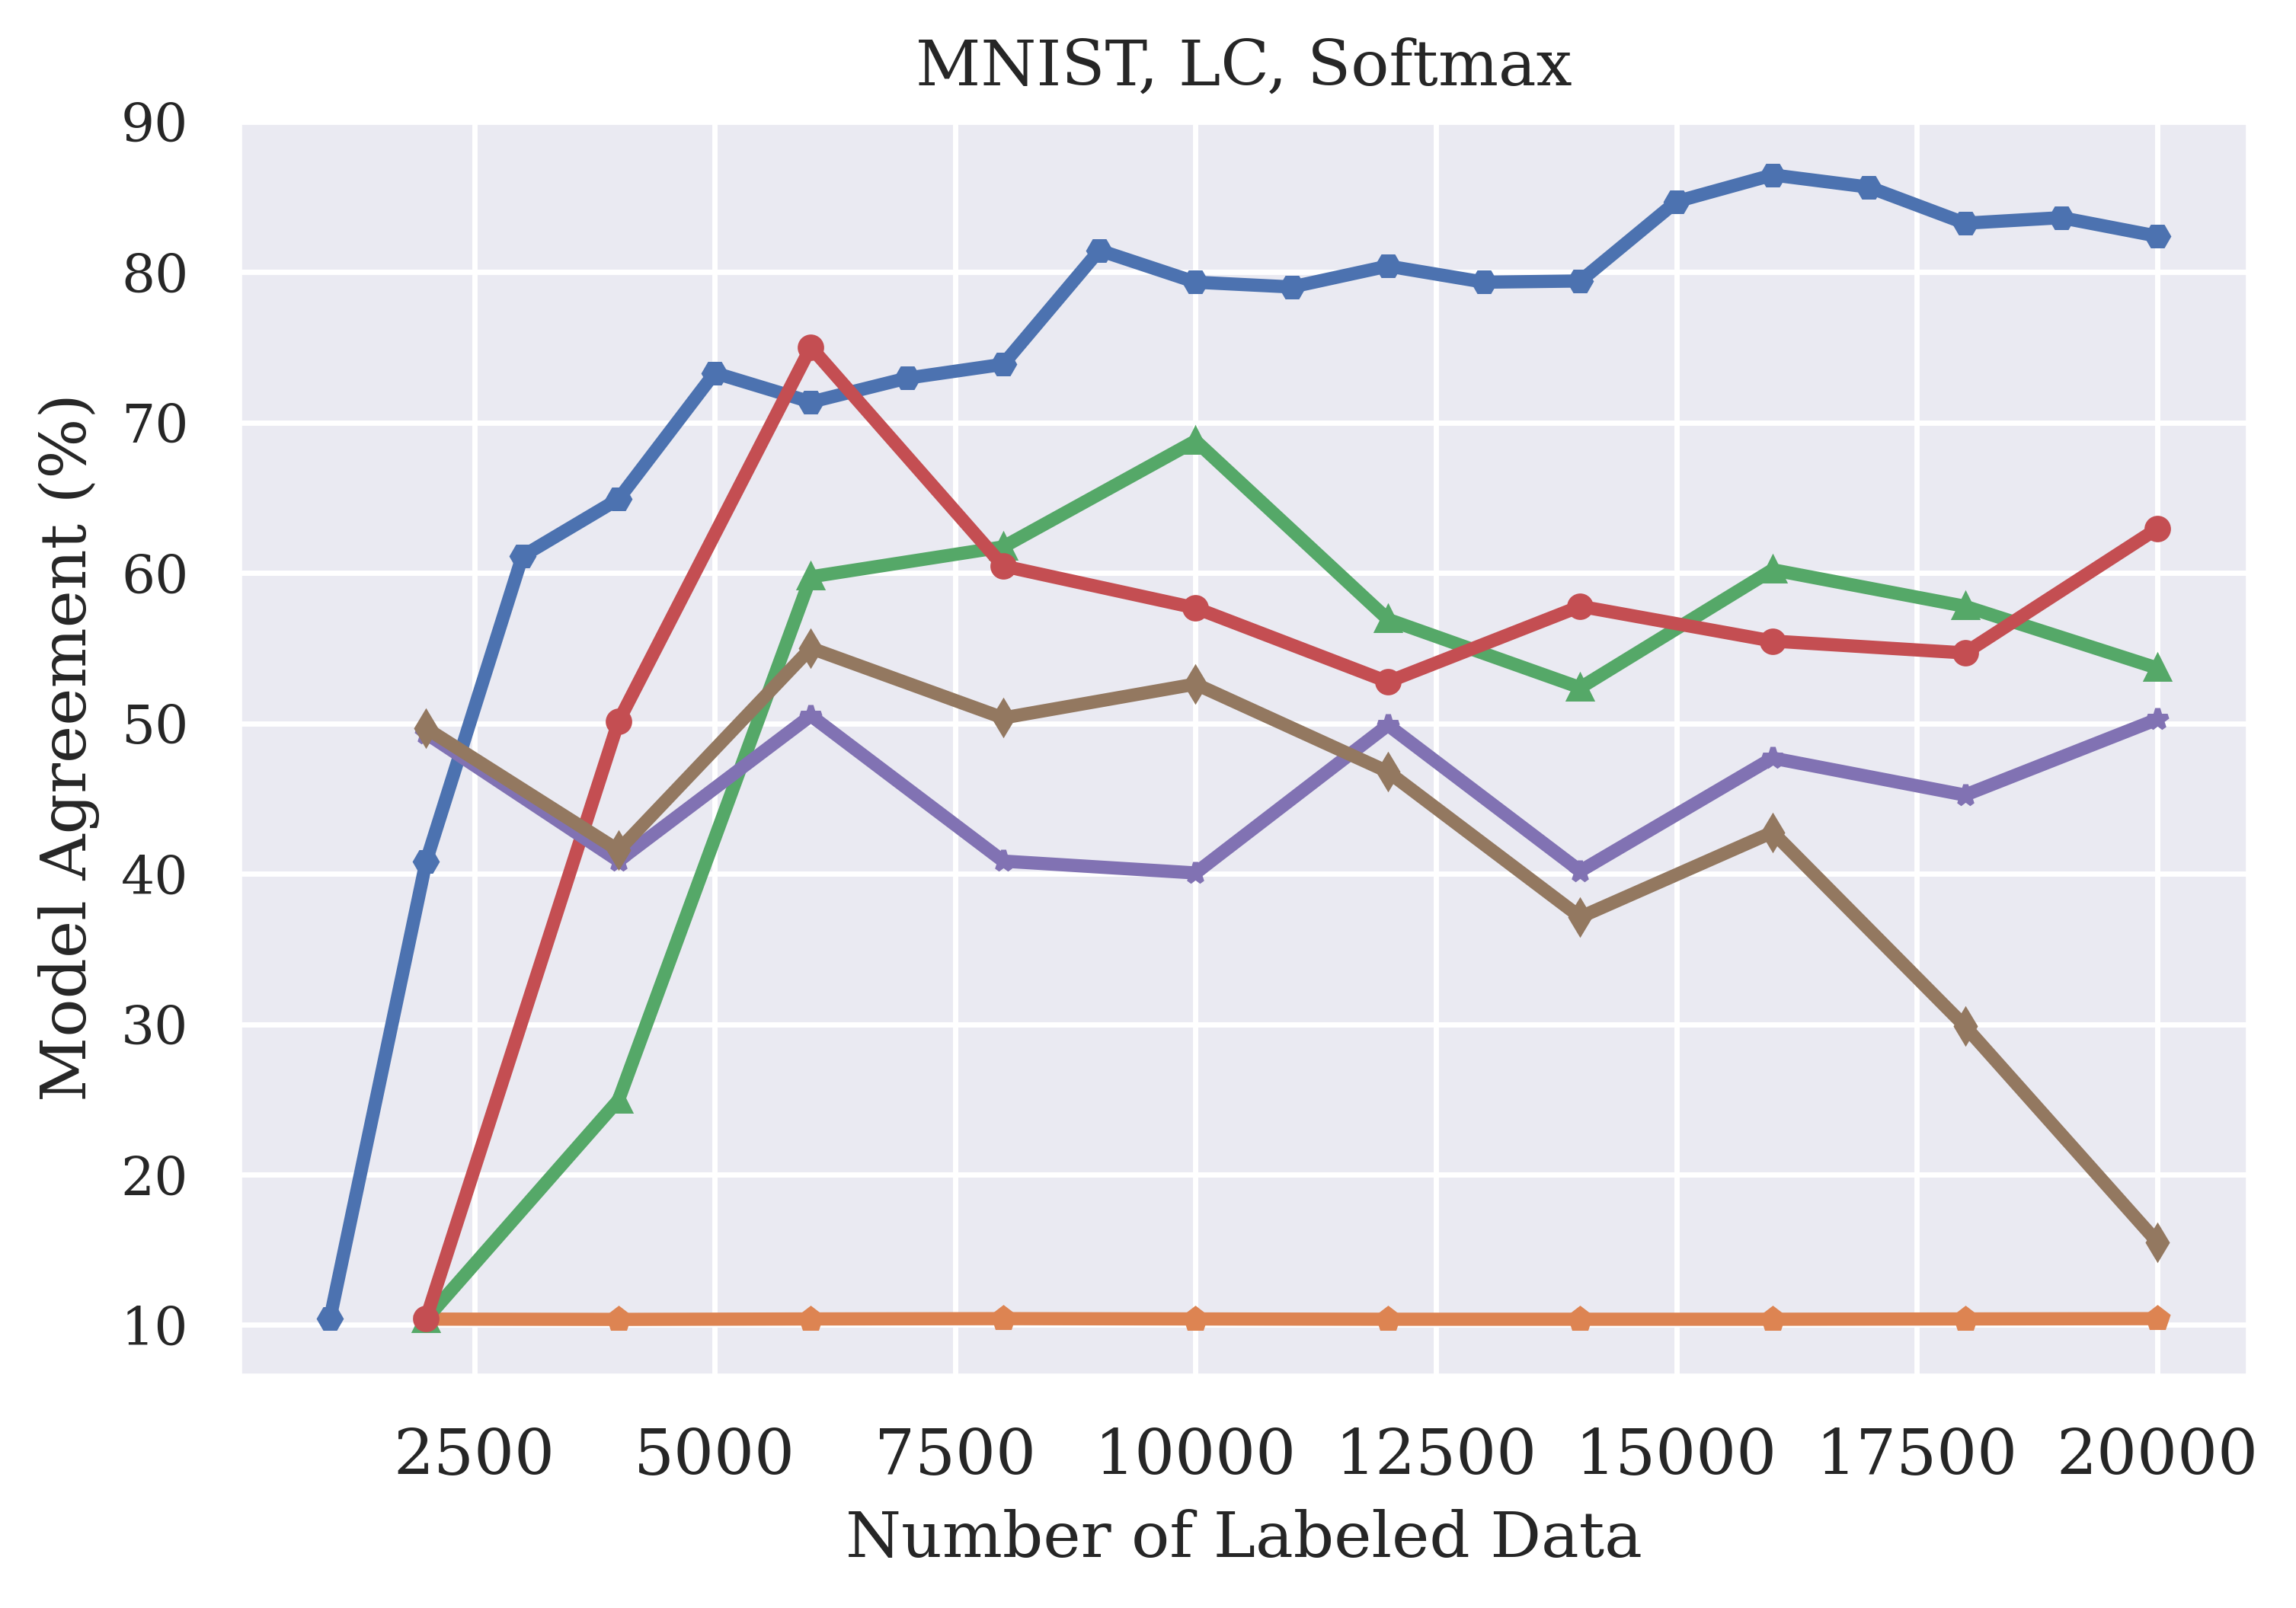
\includegraphics[width=0.5\linewidth]{images/results_CALMS/mnist_softmax_lc.png}
    \caption{Agreement Comparison for Model Stealing on MNIST using the softmax output and the Active Learning strategy \gls{lc}}
    \label{fig:CALMSMNISTSoftmaxLC}
\end{figure}

\begin{figure}[!htb]
    \centering
    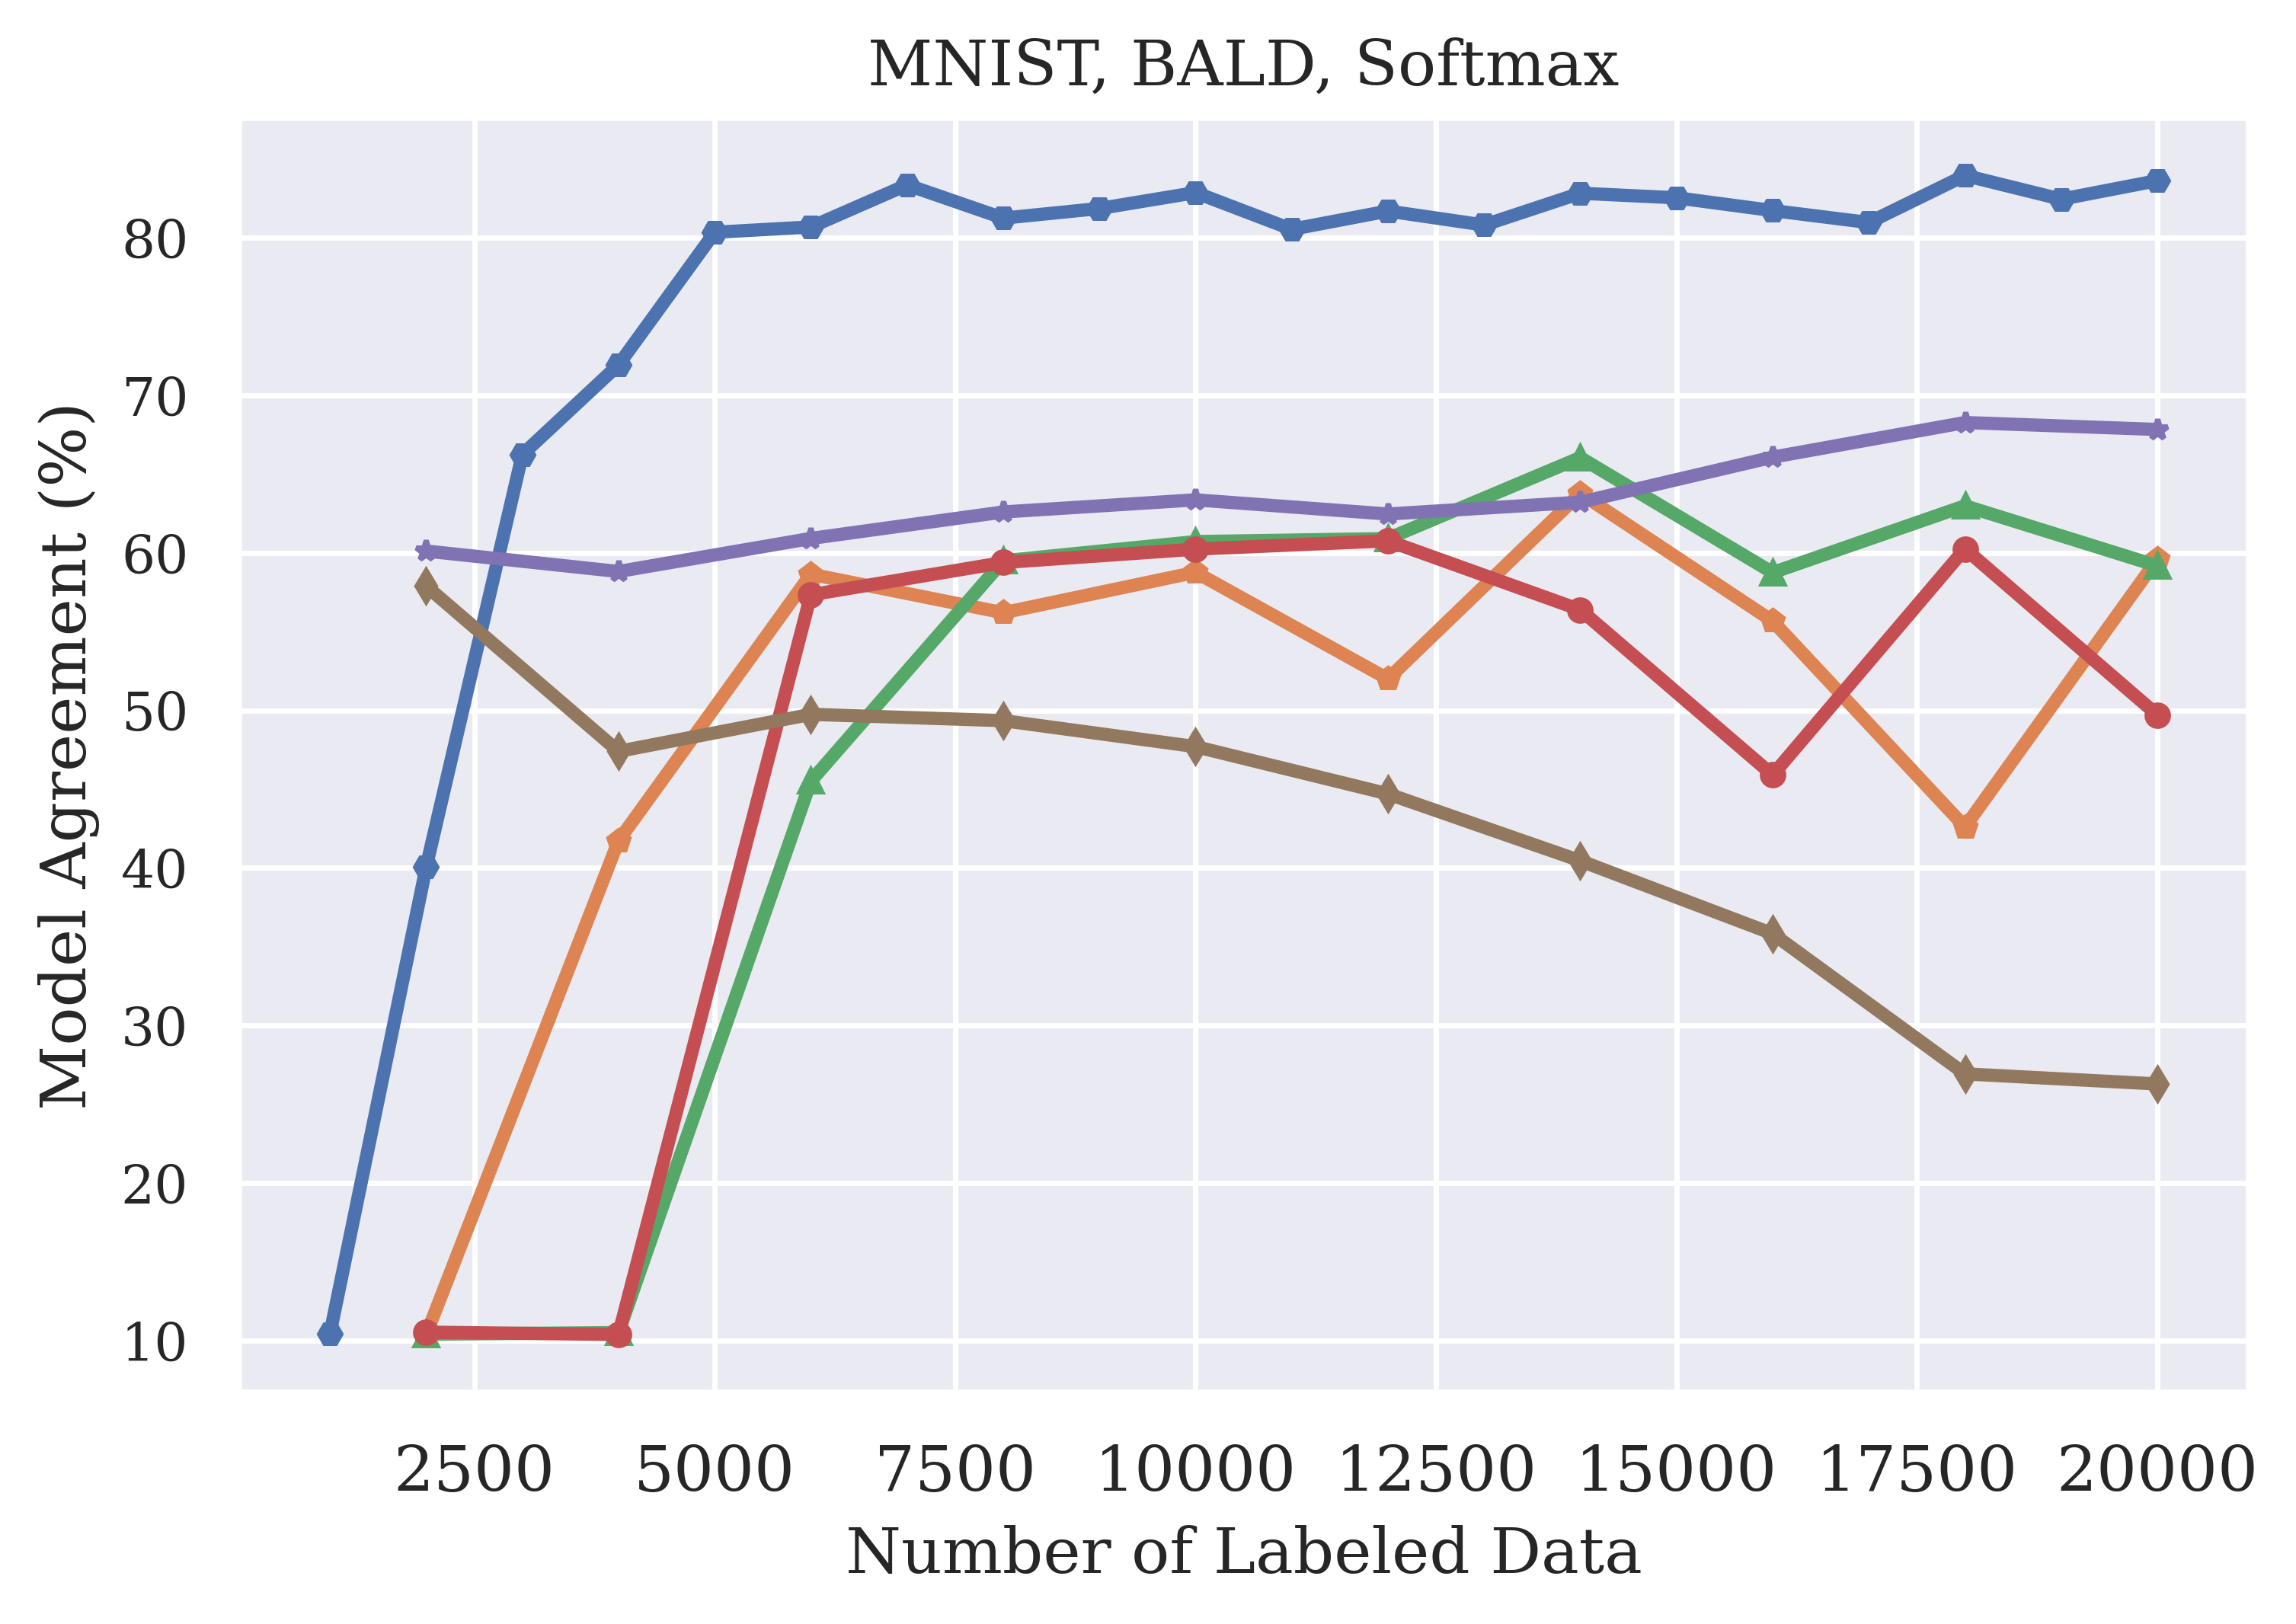
\includegraphics[width=0.5\linewidth]{images/results_CALMS/mnist_softmax_bald.png}
    \caption{Agreement Comparison for Model Stealing on MNIST using the softmax output and the Active Learning strategy \gls{bald}}
    \label{fig:CALMSMNISTSoftmaxBALD}
\end{figure}

\begin{figure}[!htb]
    \centering
    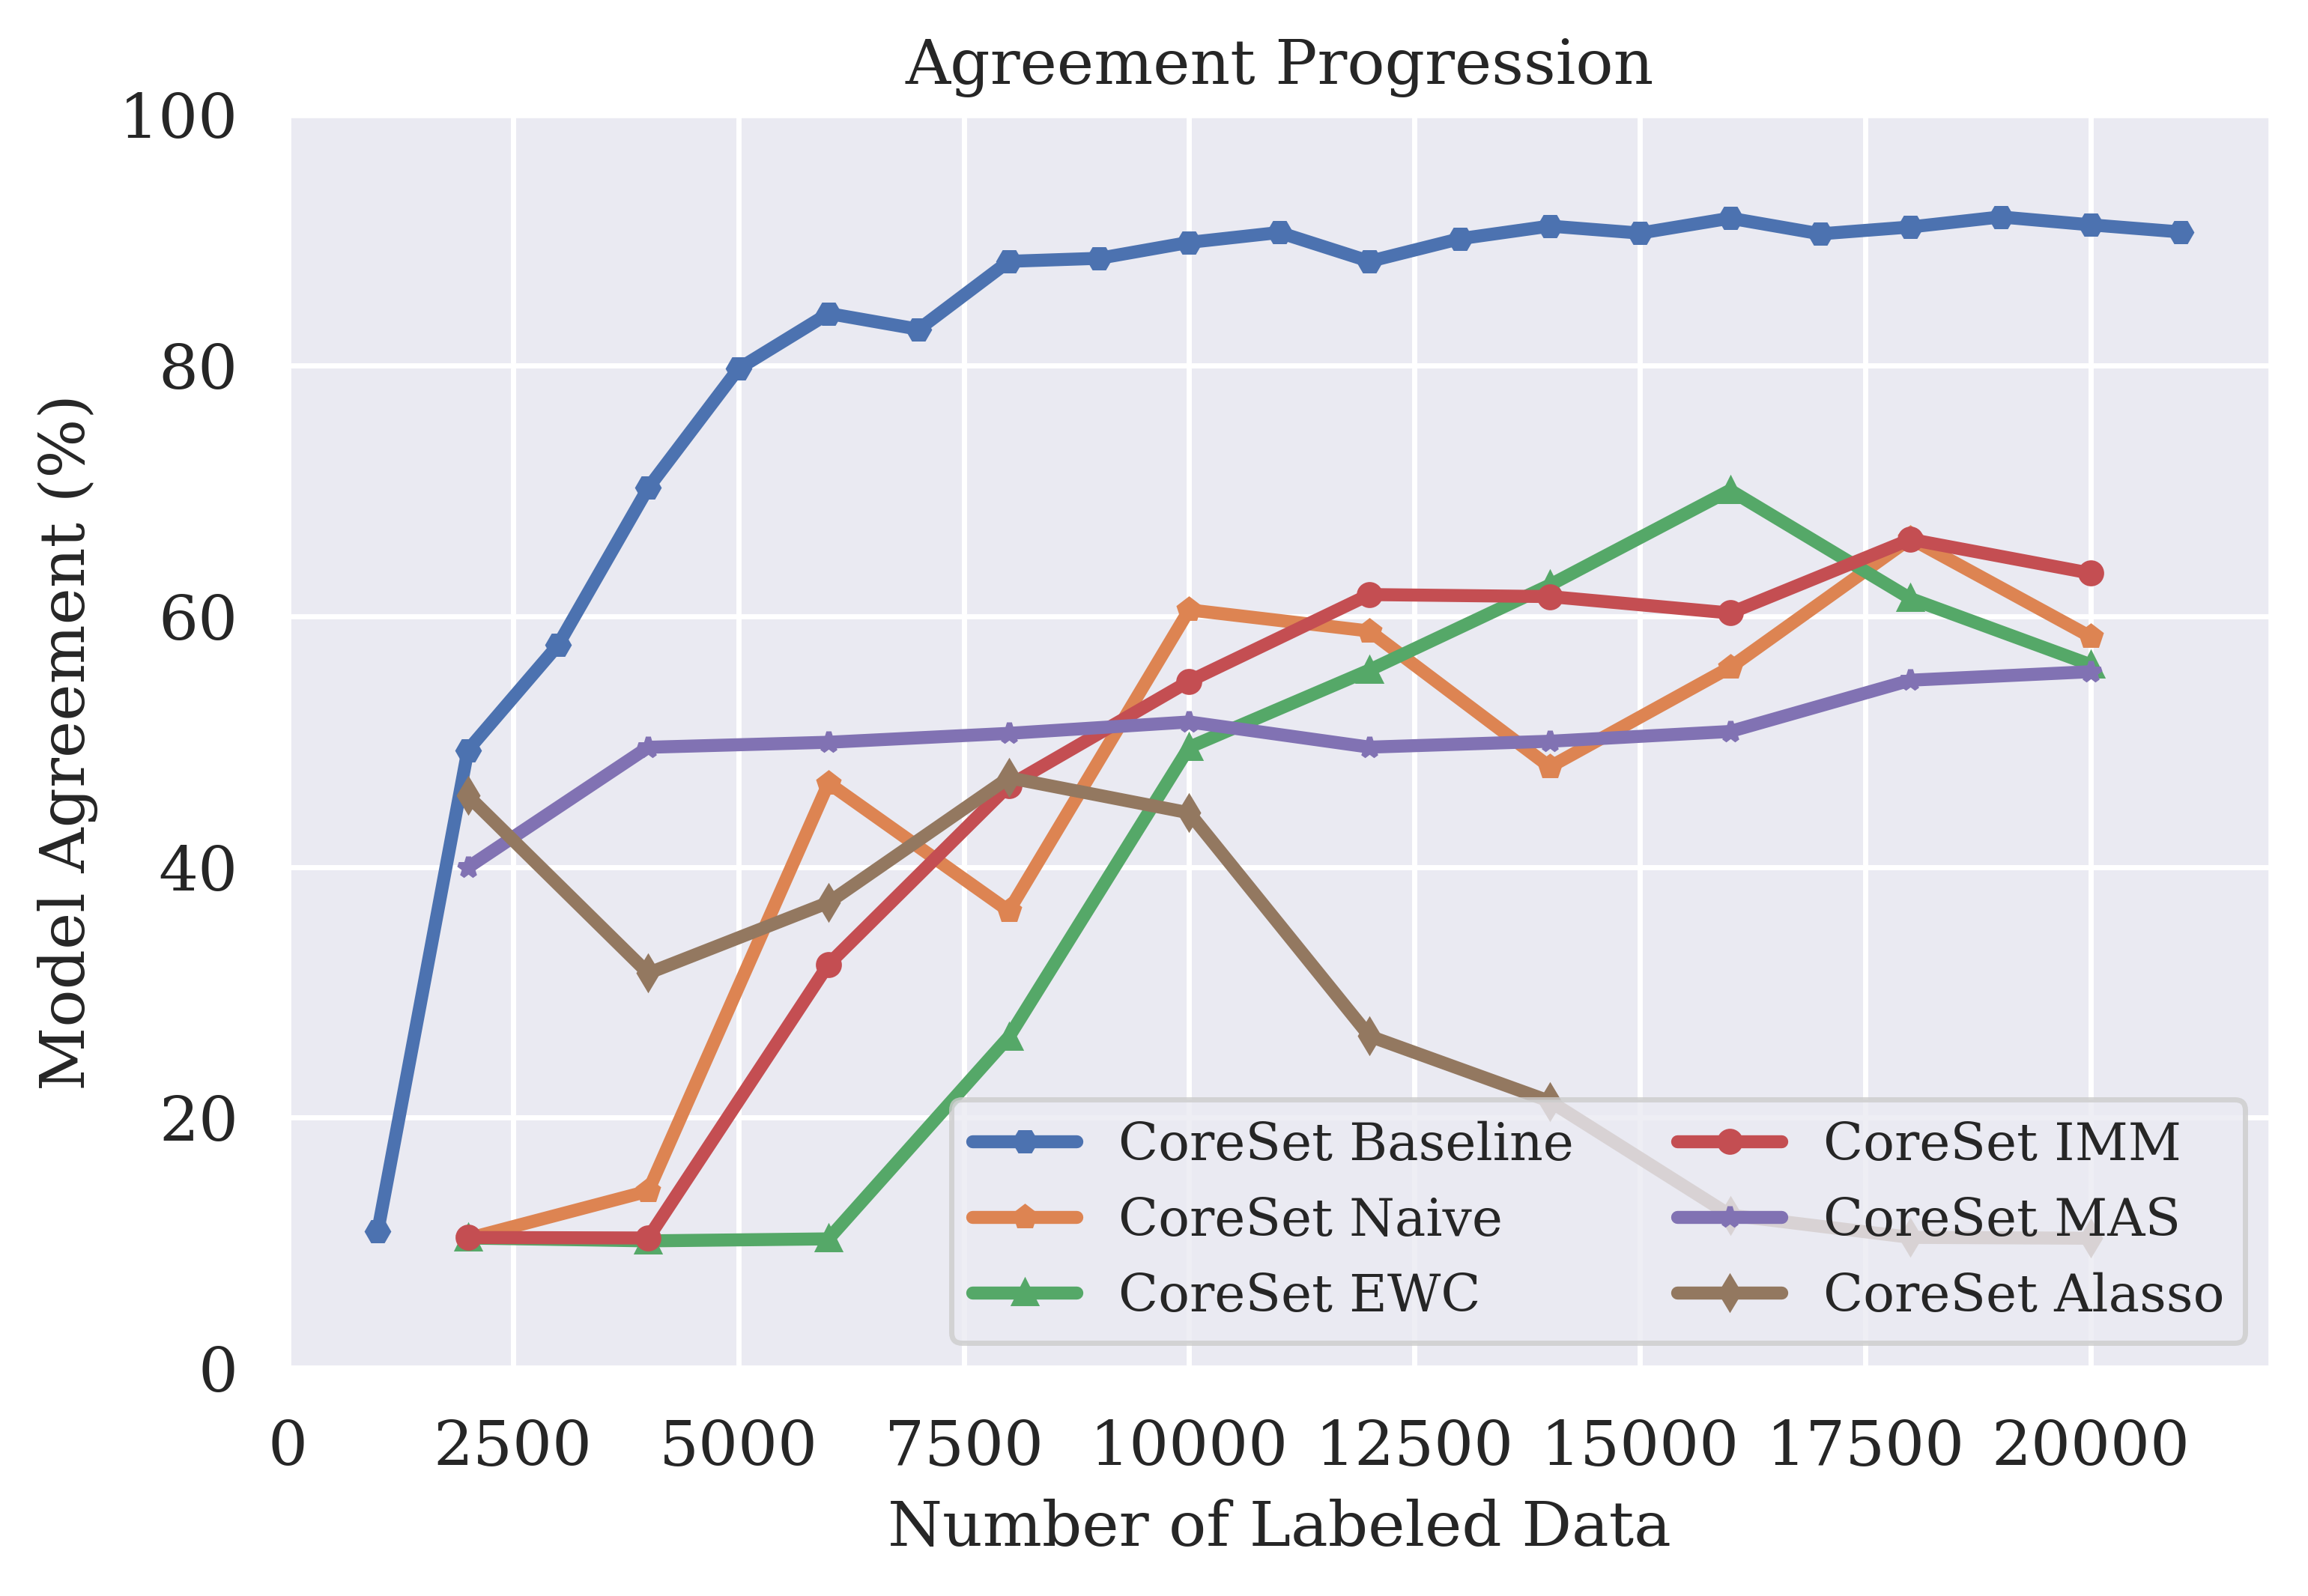
\includegraphics[width=0.5\linewidth]{images/results_CALMS/mnist_softmax_coreset.png}
    \caption{Agreement Comparison for Model Stealing on MNIST using the softmax output and the Active Learning strategy CoreSet}
    \label{fig:CALMSMNISTSoftmaxCoreSet}
\end{figure}

\begin{figure}[!htb]
    \centering
    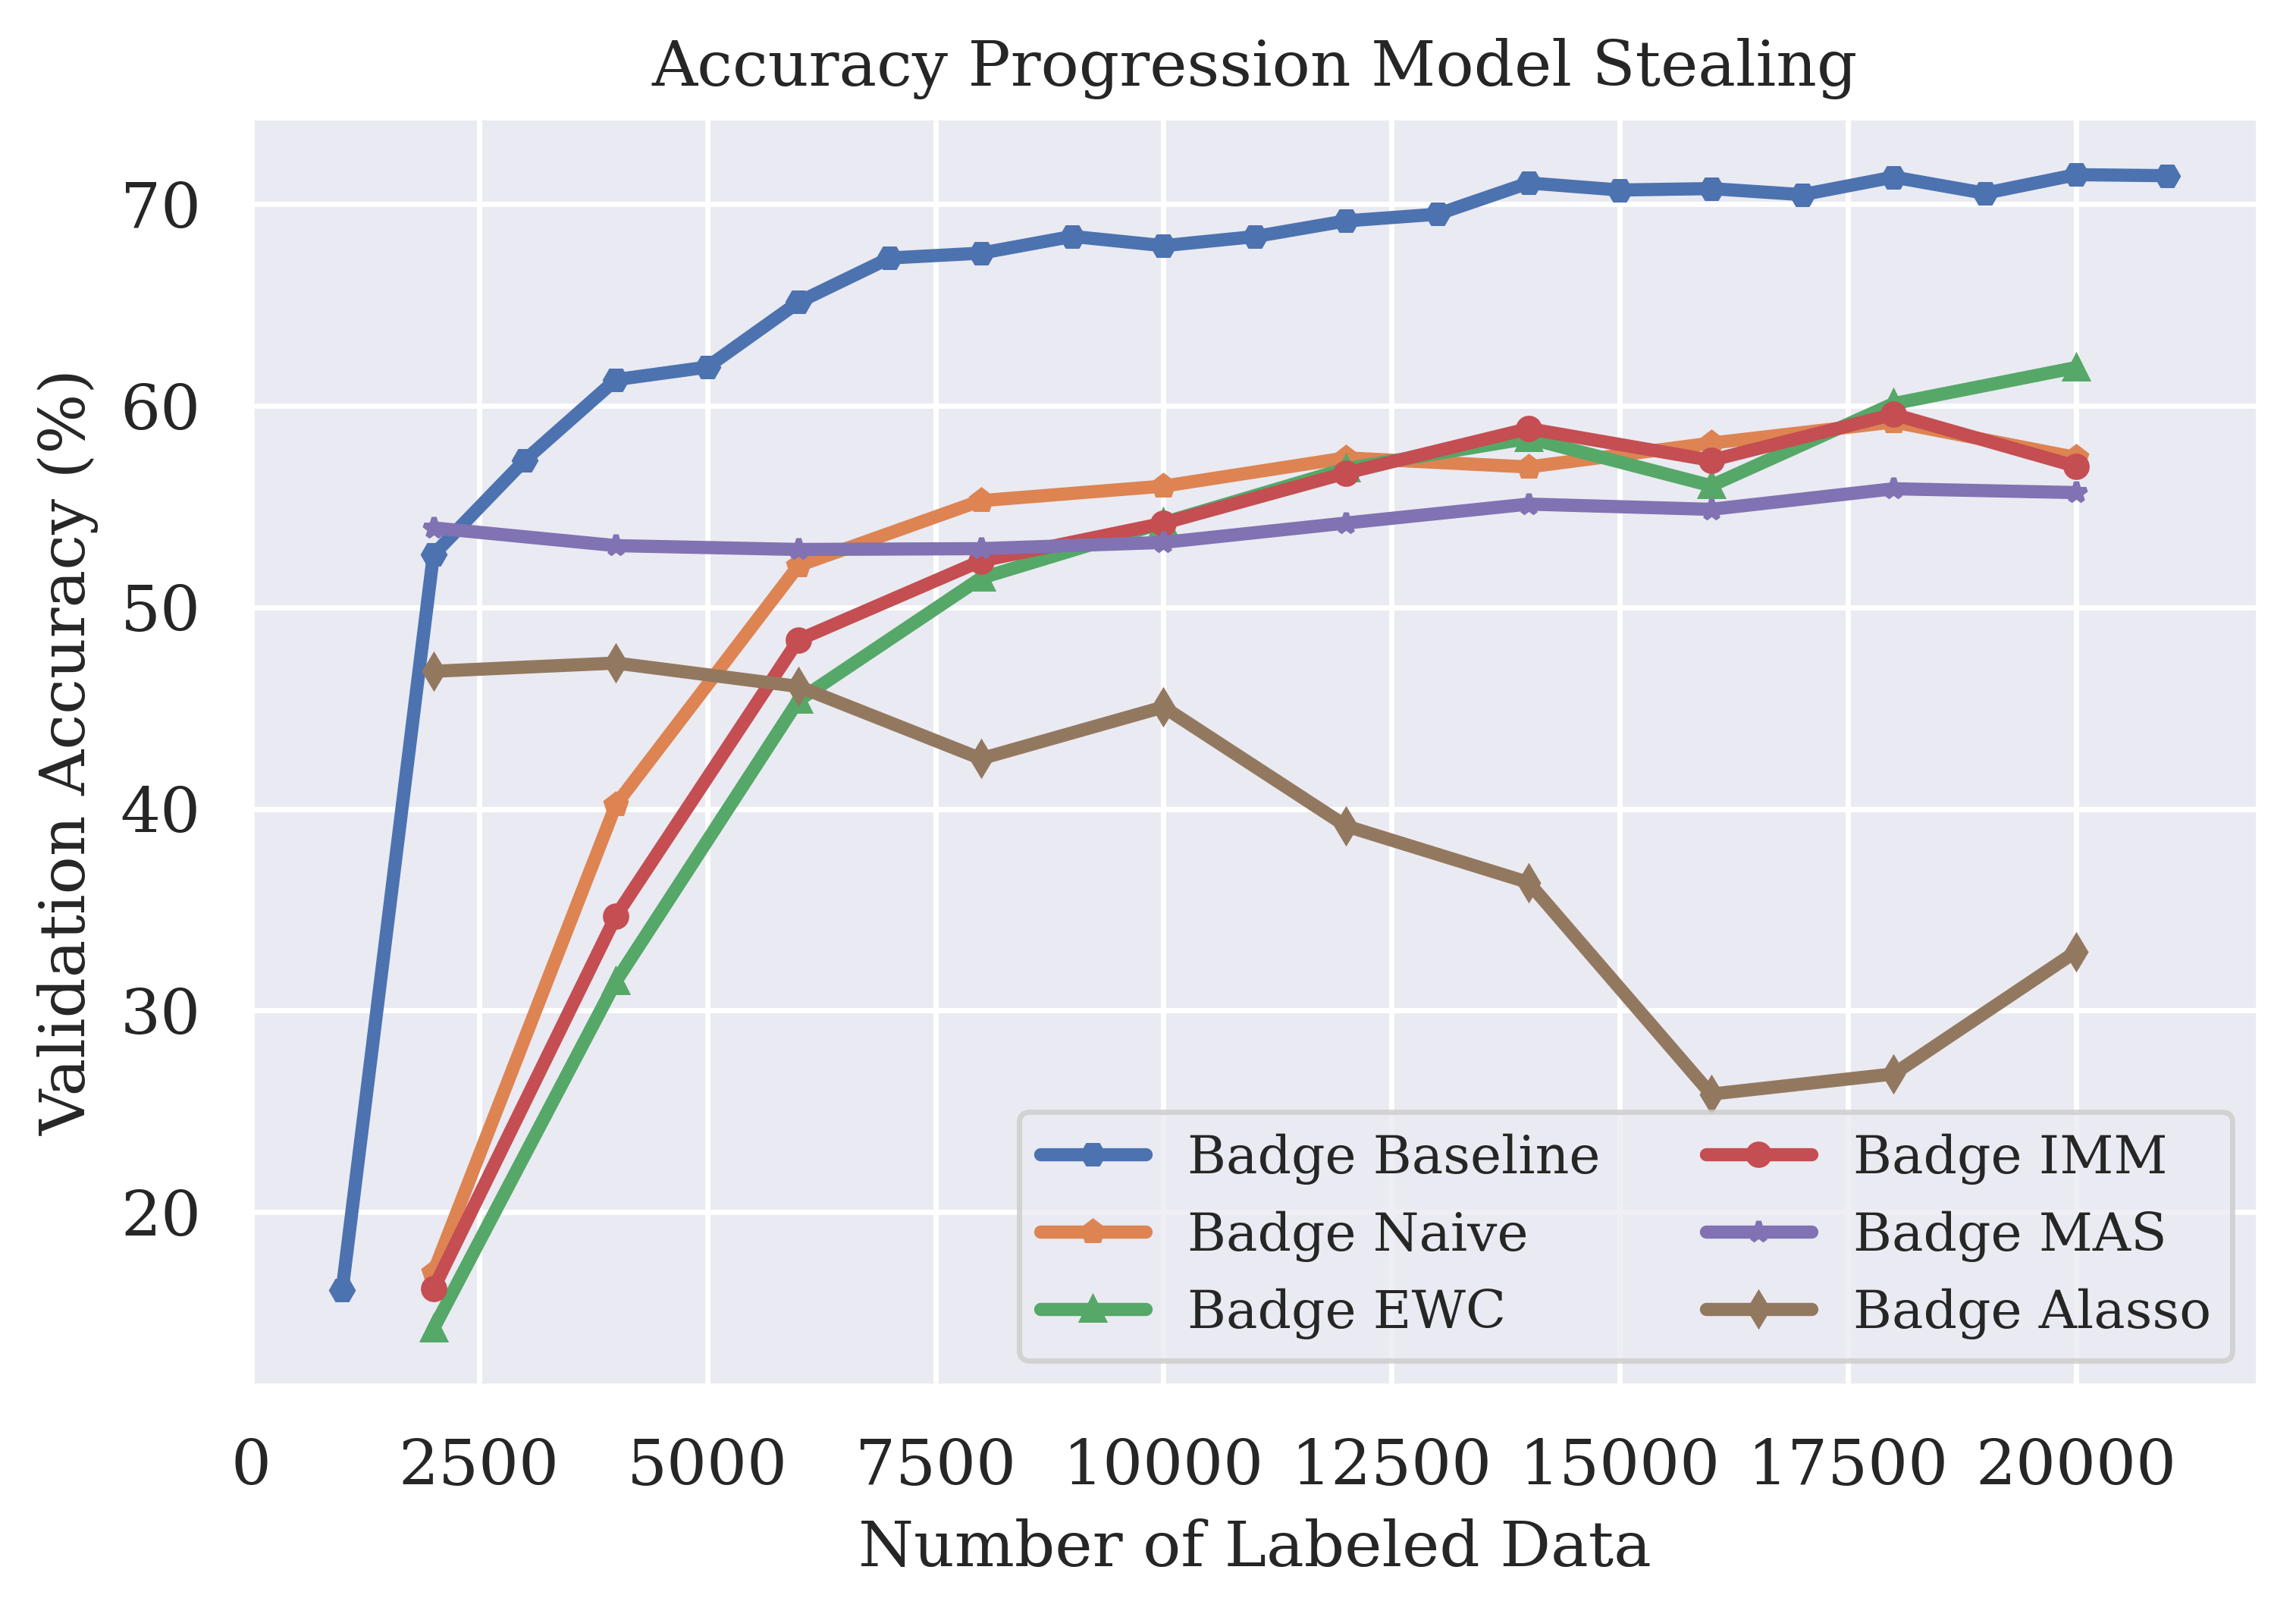
\includegraphics[width=0.5\linewidth]{images/results_CALMS/cifar_softmax_badge.png}
    \caption{Agreement Comparison for Model Stealing on MNIST using the softmax output and the Active Learning strategy \gls{badge}}
    \label{fig:CALMSMNISTSoftmaxBadge}
\end{figure}

\subsubsection{CIFAR-10}
\label{sec:Appendix:CALMS:CIFAR}
In this section, we present the full runs of all experiments which involve Continual Active Learning using CIFAR-10 as a Target Model Dataset.
%Label
\begin{figure}[!htb]
    \centering
    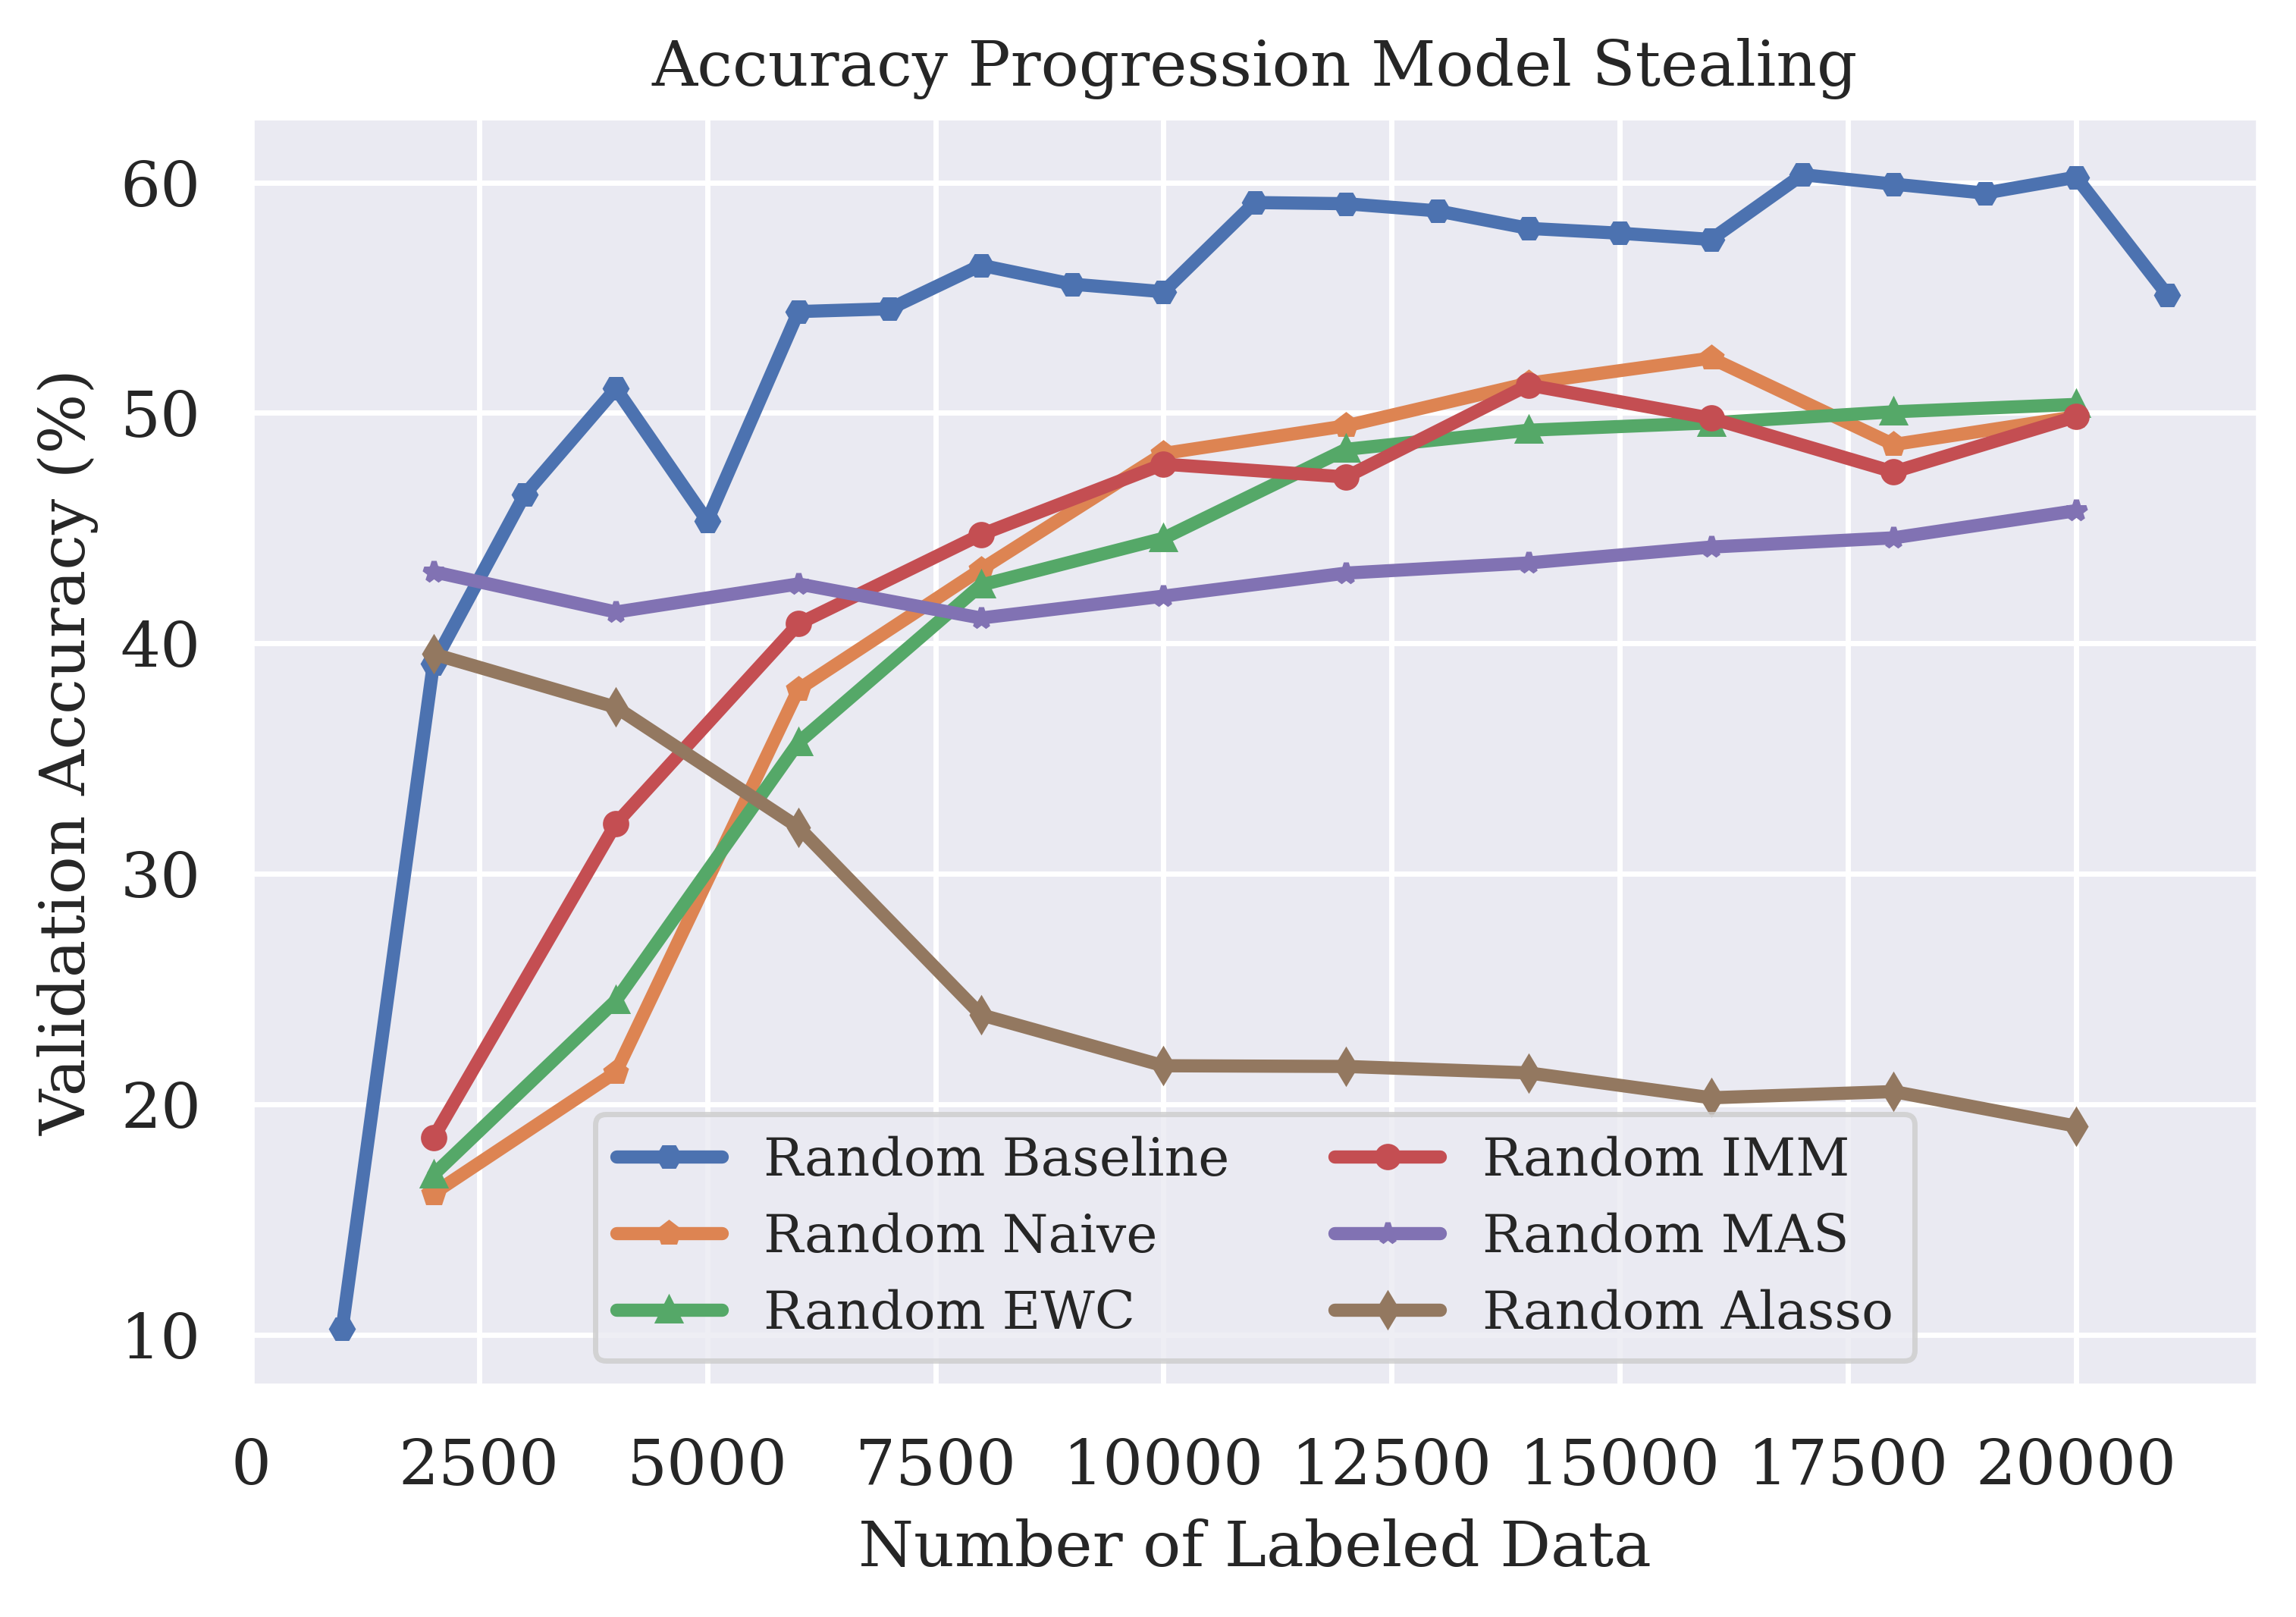
\includegraphics[width=0.5\linewidth]{images/results_CALMS/cifar_label_random.png}
    \caption{Agreement Comparison for Model Stealing on CIFAR-10 using the predicted class label and the Active Learning strategy Random}
    \label{fig:CALMSCIFAR10LabelRandom}
\end{figure}

\begin{figure}[!htb]
    \centering
    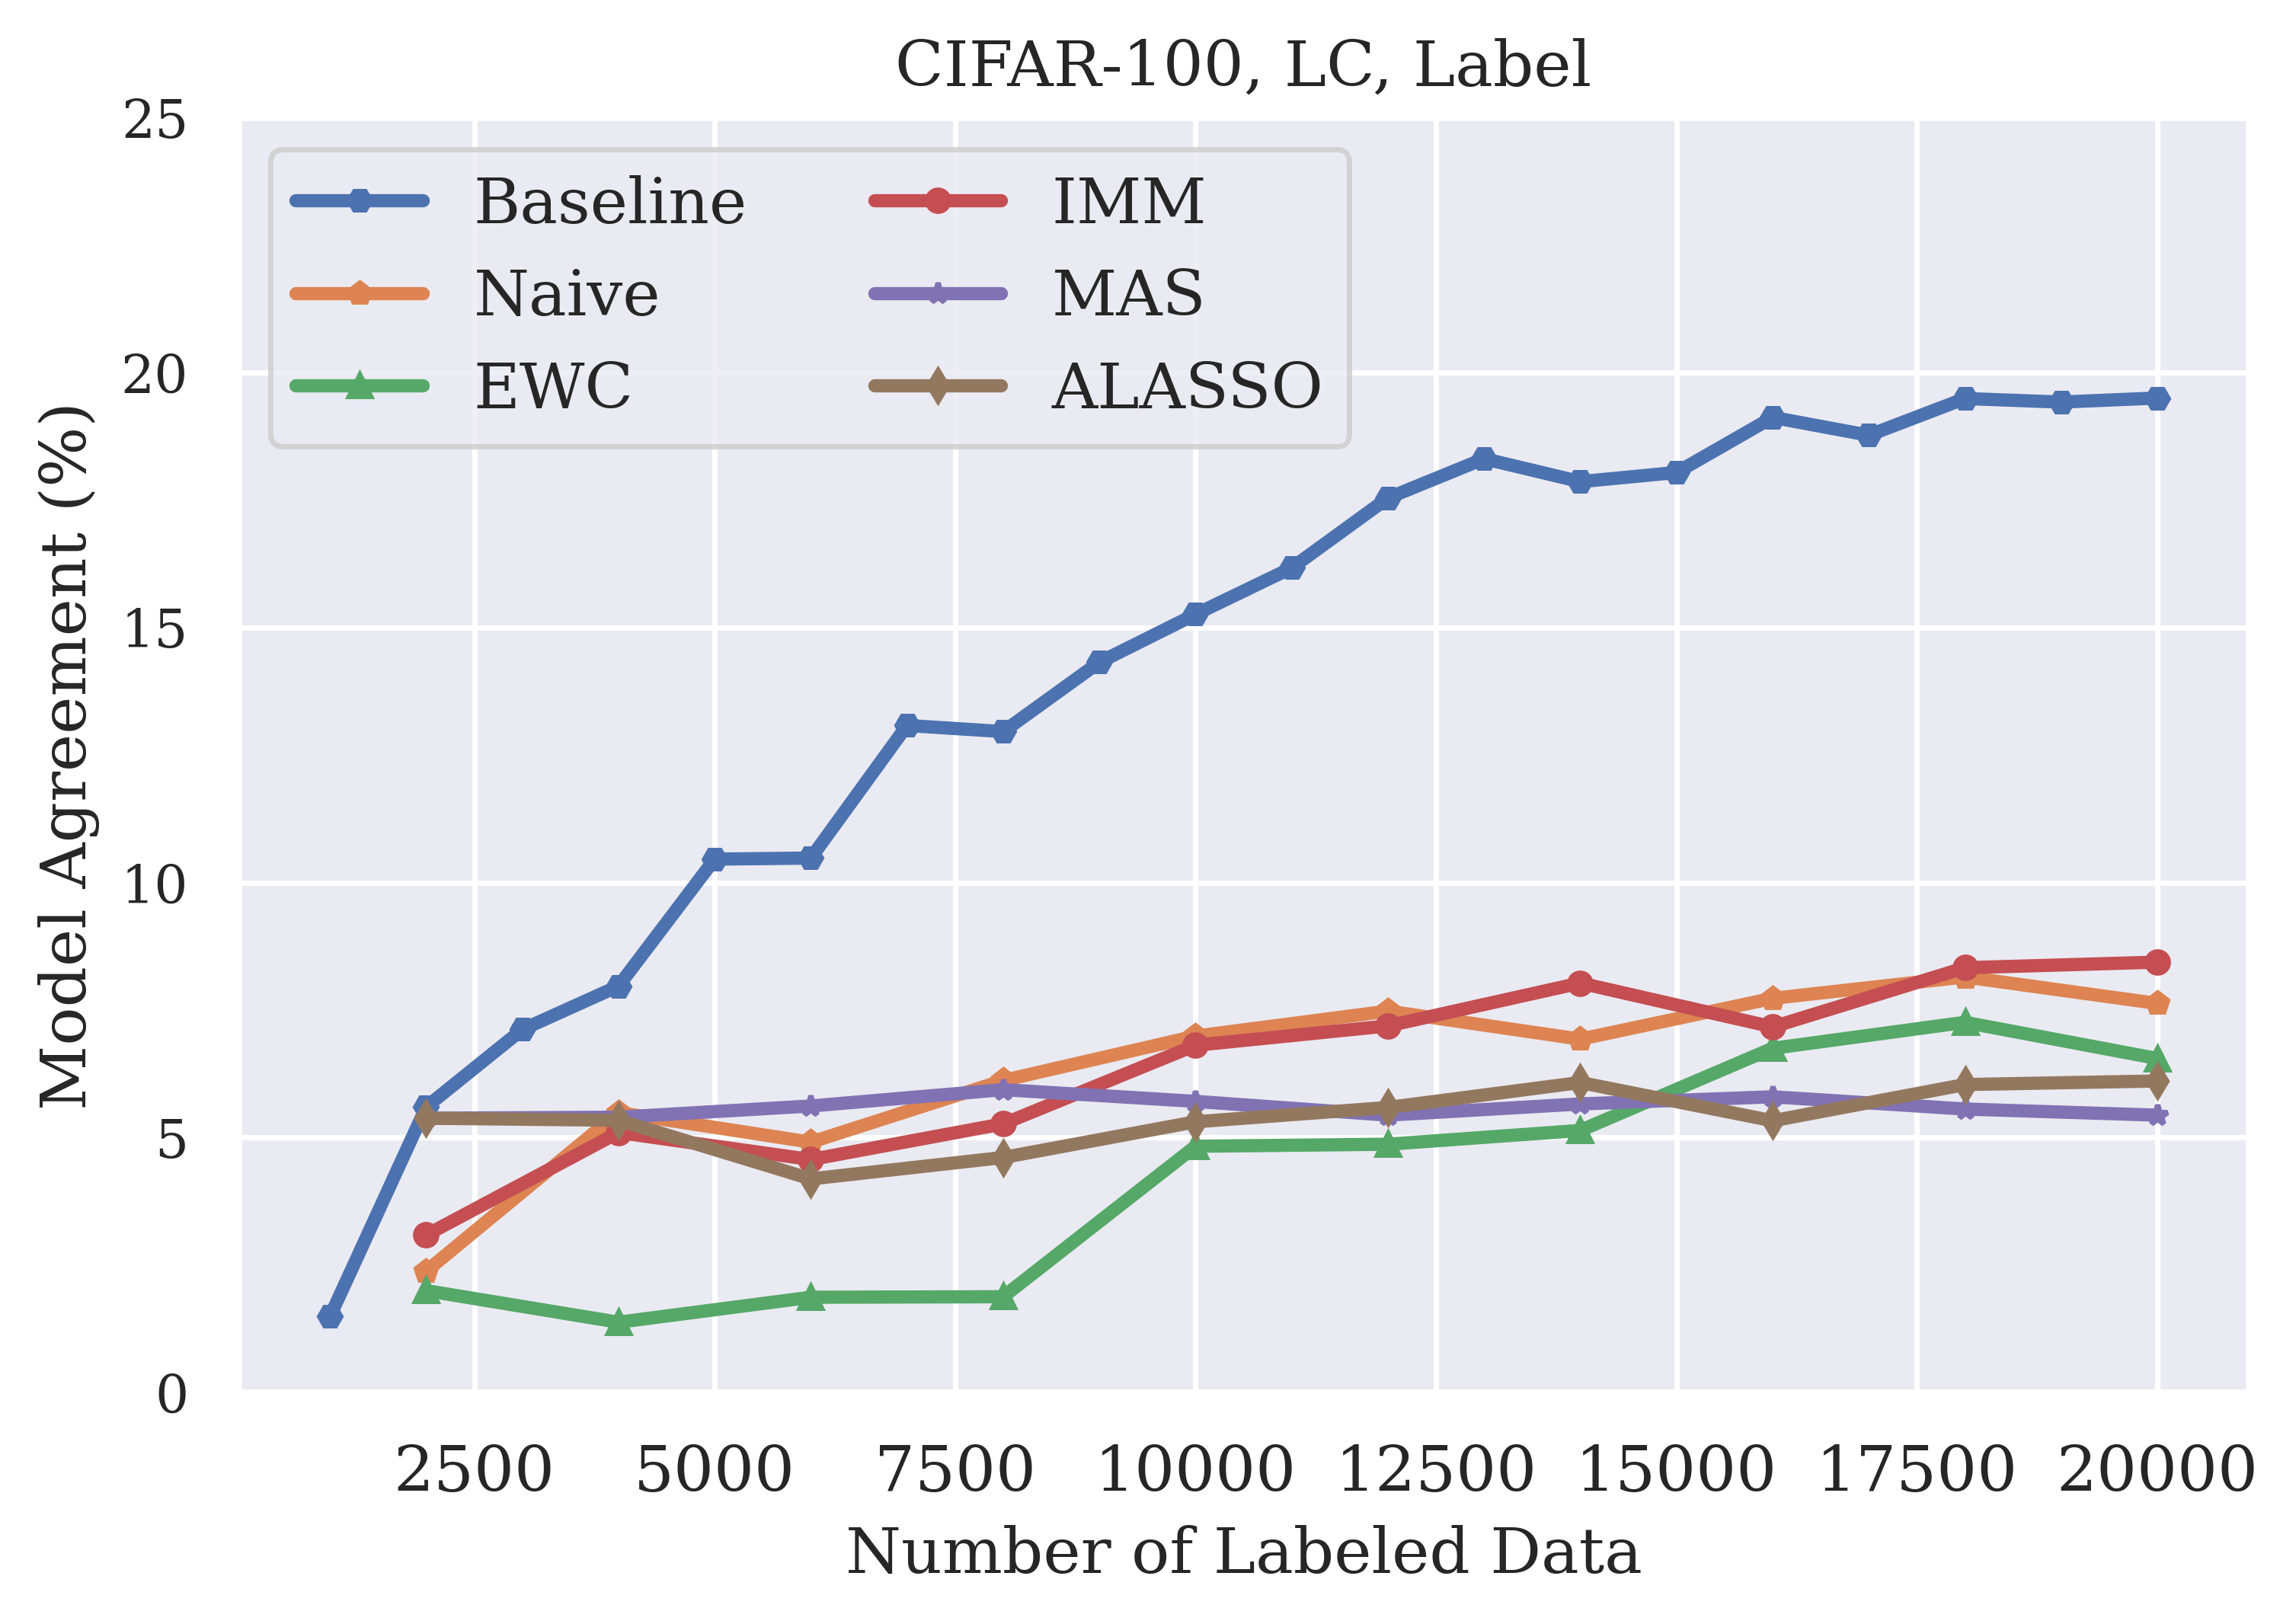
\includegraphics[width=0.5\linewidth]{images/results_CALMS/cifar100_label_lc.png}
    \caption{Agreement Comparison for Model Stealing on CIFAR-10 using the predicted class label and the Active Learning strategy \gls{lc}}
    \label{fig:CALMSCIFAR10LabelLC}
\end{figure}

\begin{figure}[!htb]
    \centering
    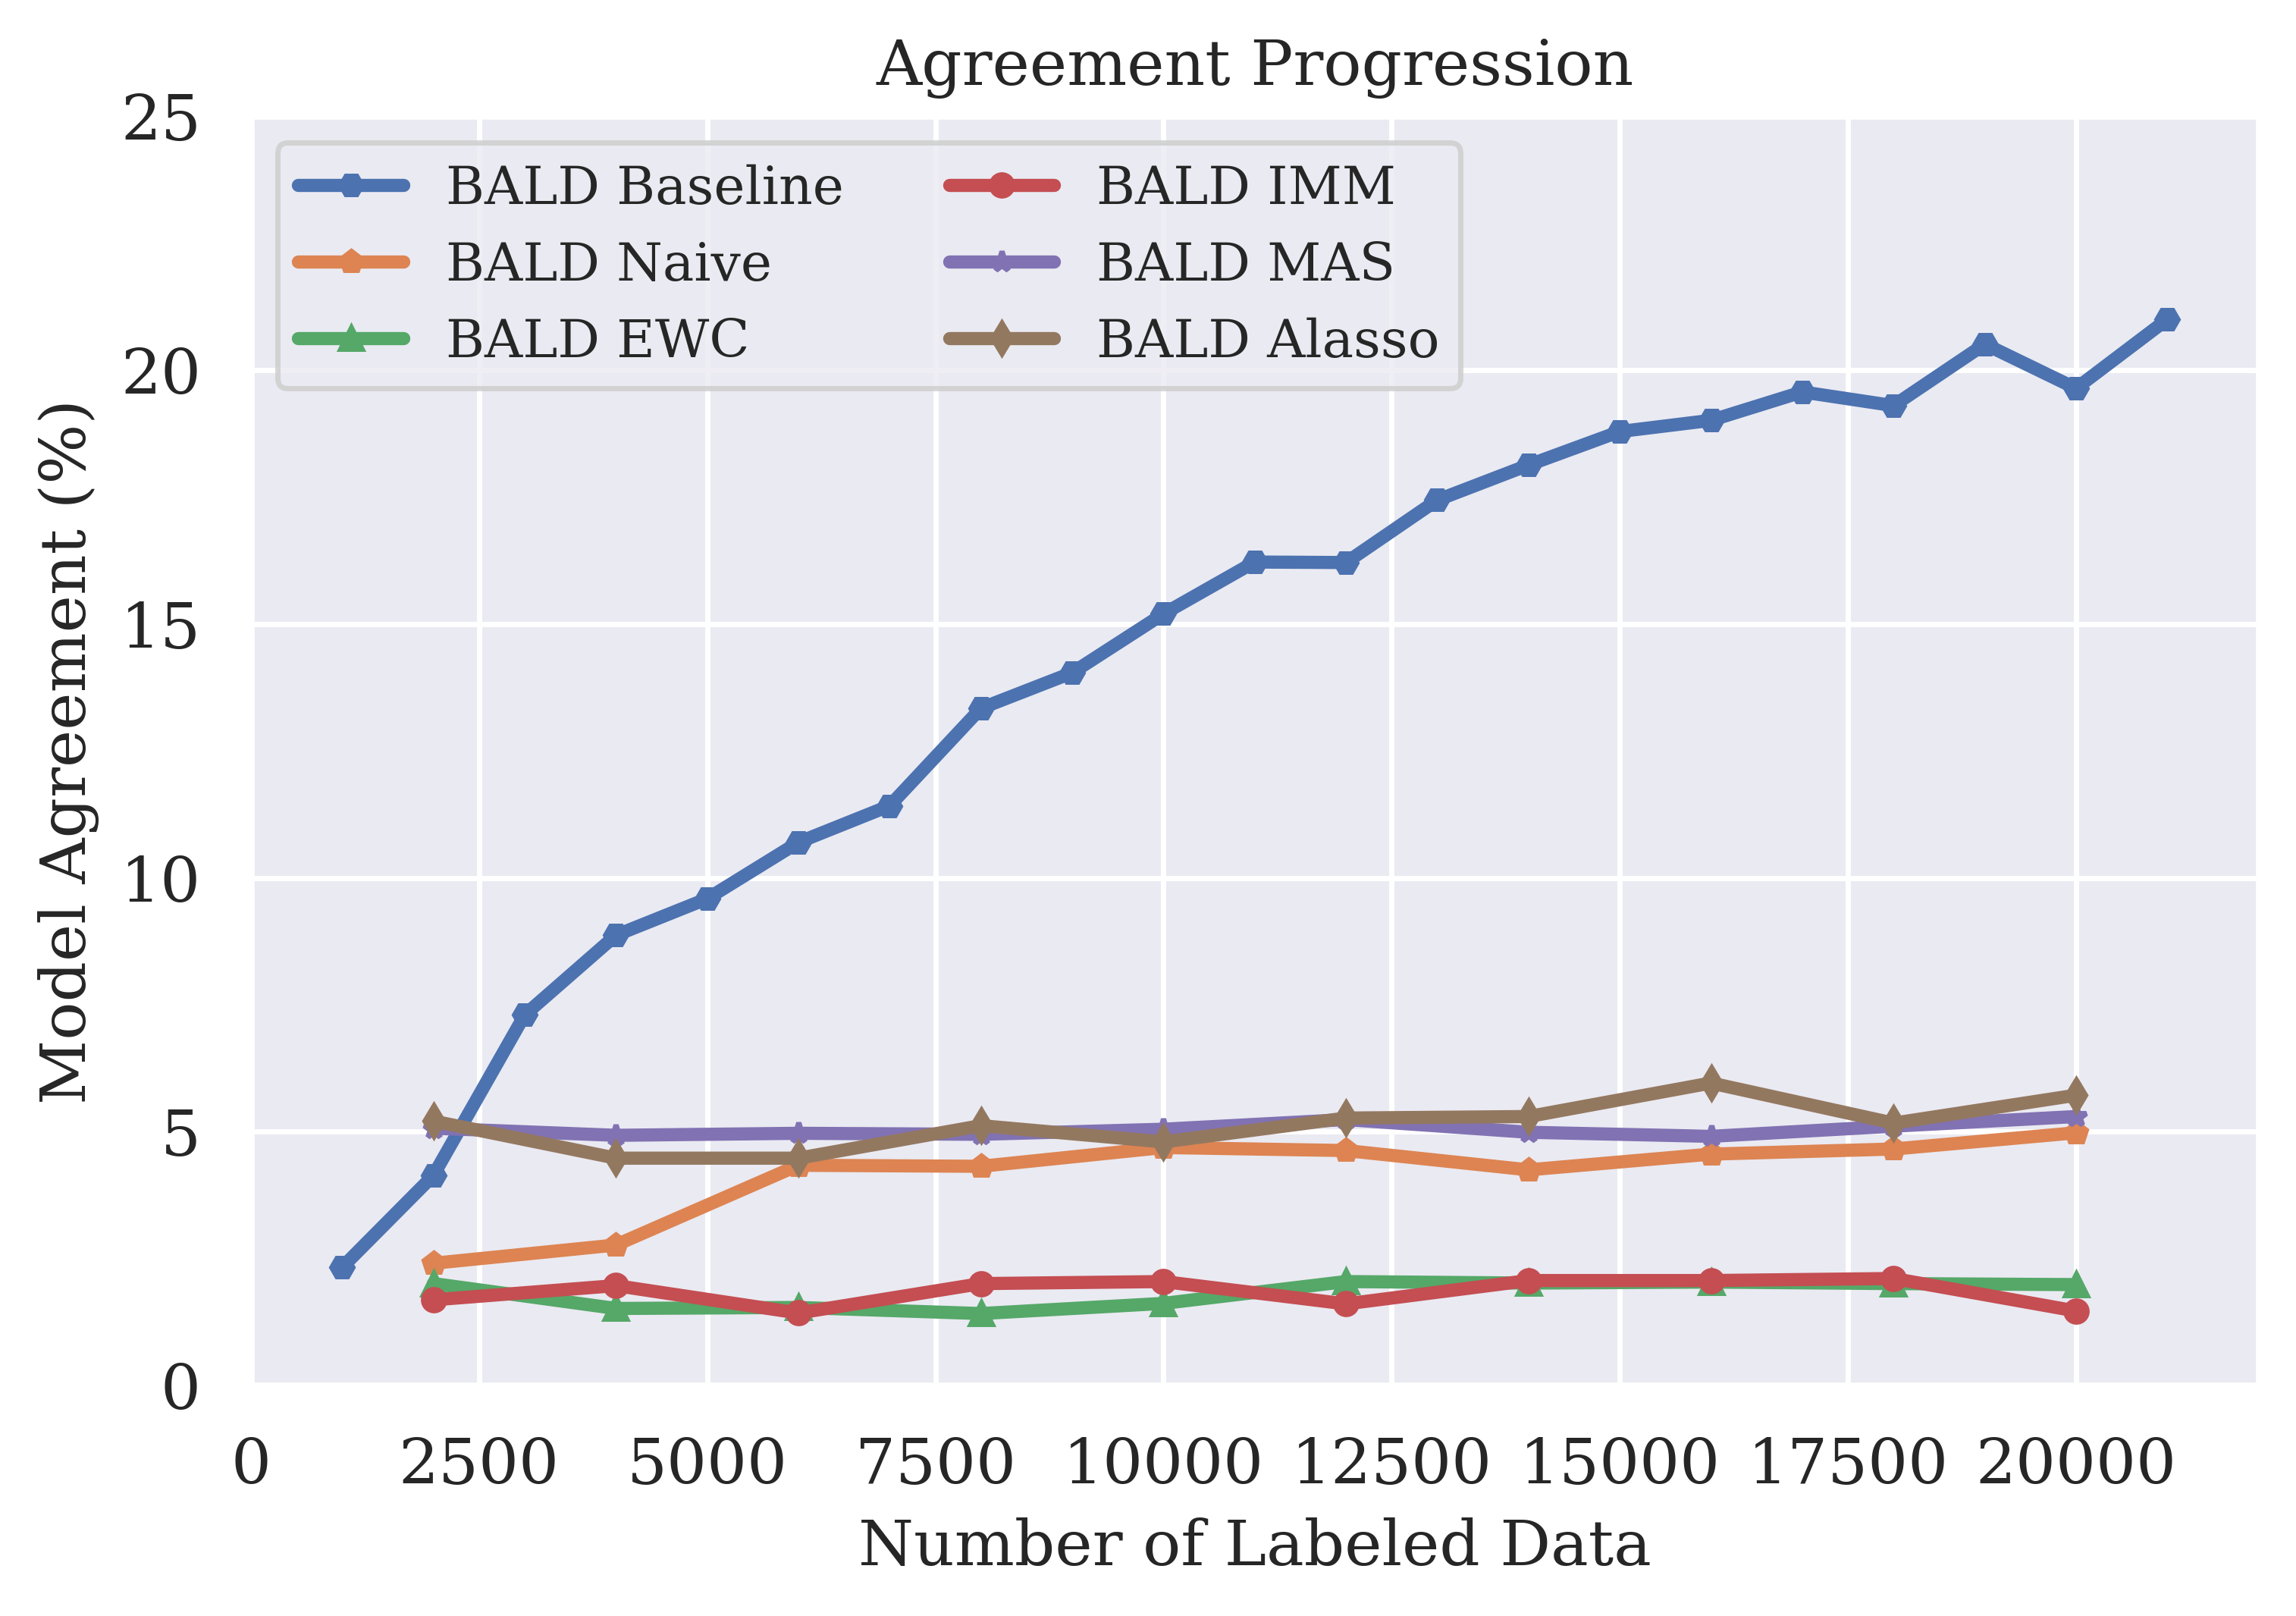
\includegraphics[width=0.5\linewidth]{images/results_CALMS/cifar100_label_bald.png}
    \caption{Agreement Comparison for Model Stealing on CIFAR-10 using the predicted class label and the Active Learning strategy \gls{bald}}
    \label{fig:CALMSCIFAR10LabelBALD}
\end{figure}

\begin{figure}[!htb]
    \centering
    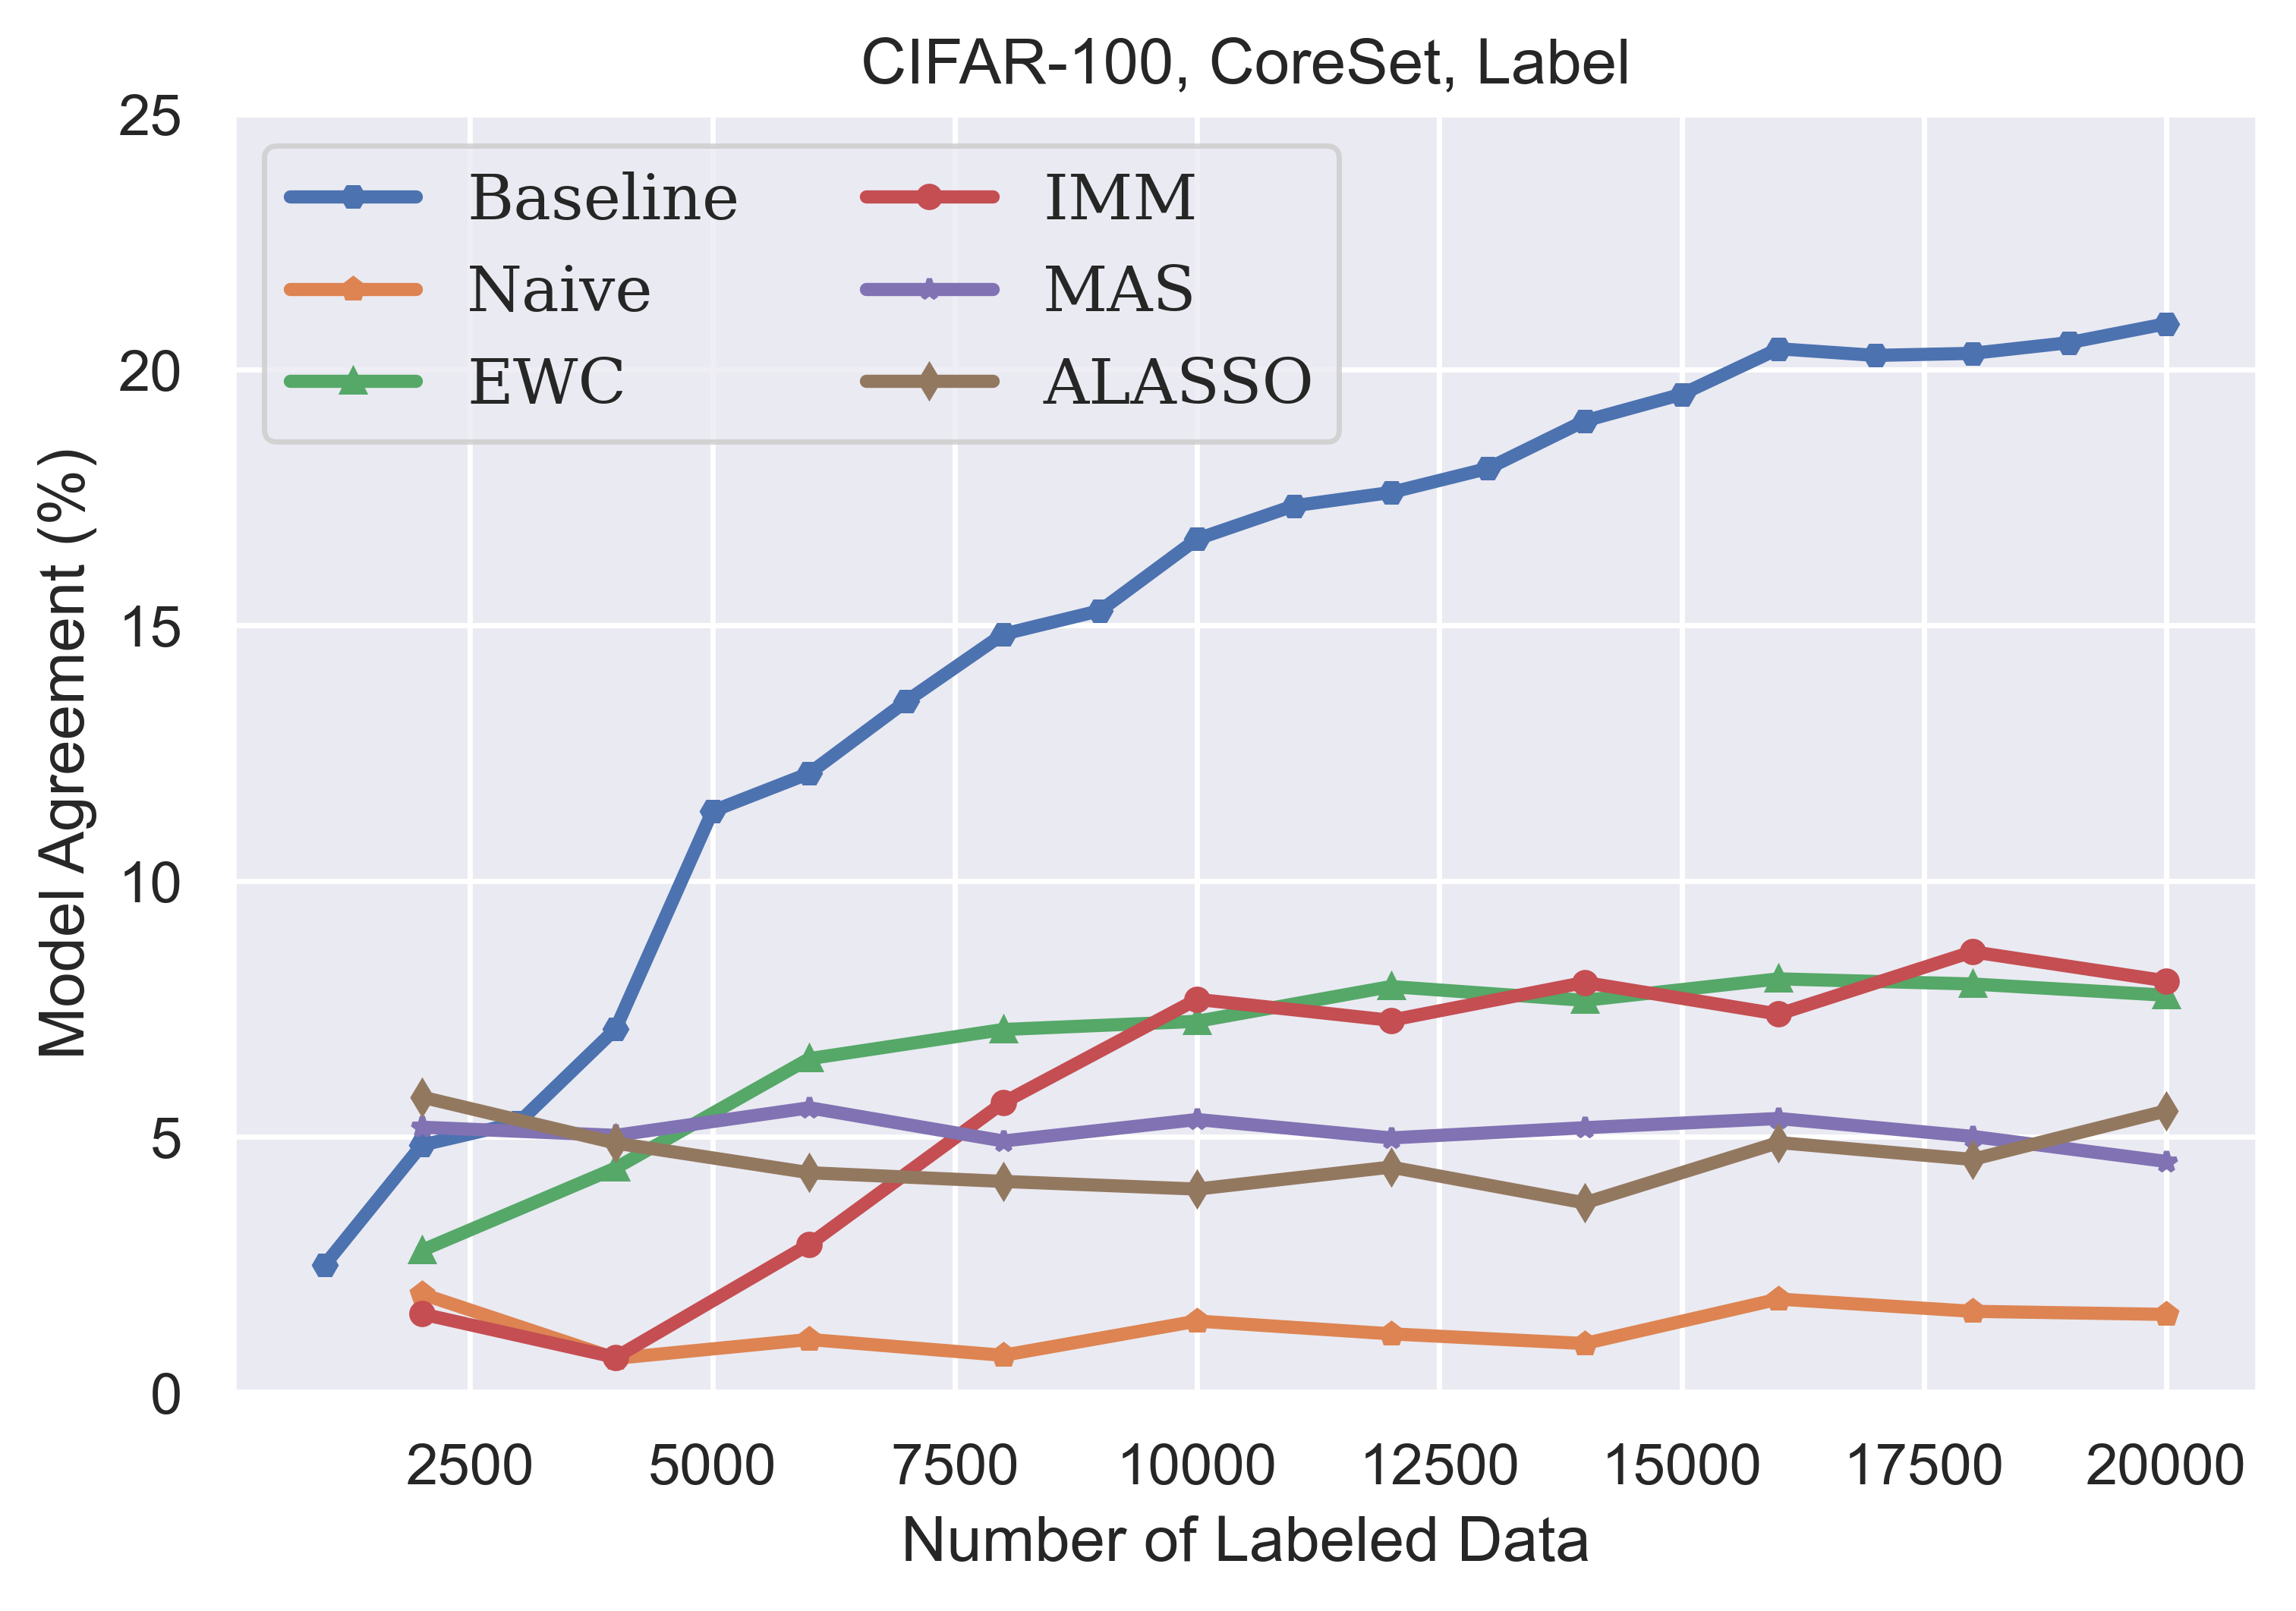
\includegraphics[width=0.5\linewidth]{images/results_CALMS/cifar100_label_coreset.png}
    \caption{Agreement Comparison for Model Stealing on CIFAR-10 using the predicted class label and the Active Learning strategy CoreSet}
    \label{fig:CALMSCIFAR10LabelCoreSet}
\end{figure}

\begin{figure}[!htb]
    \centering
    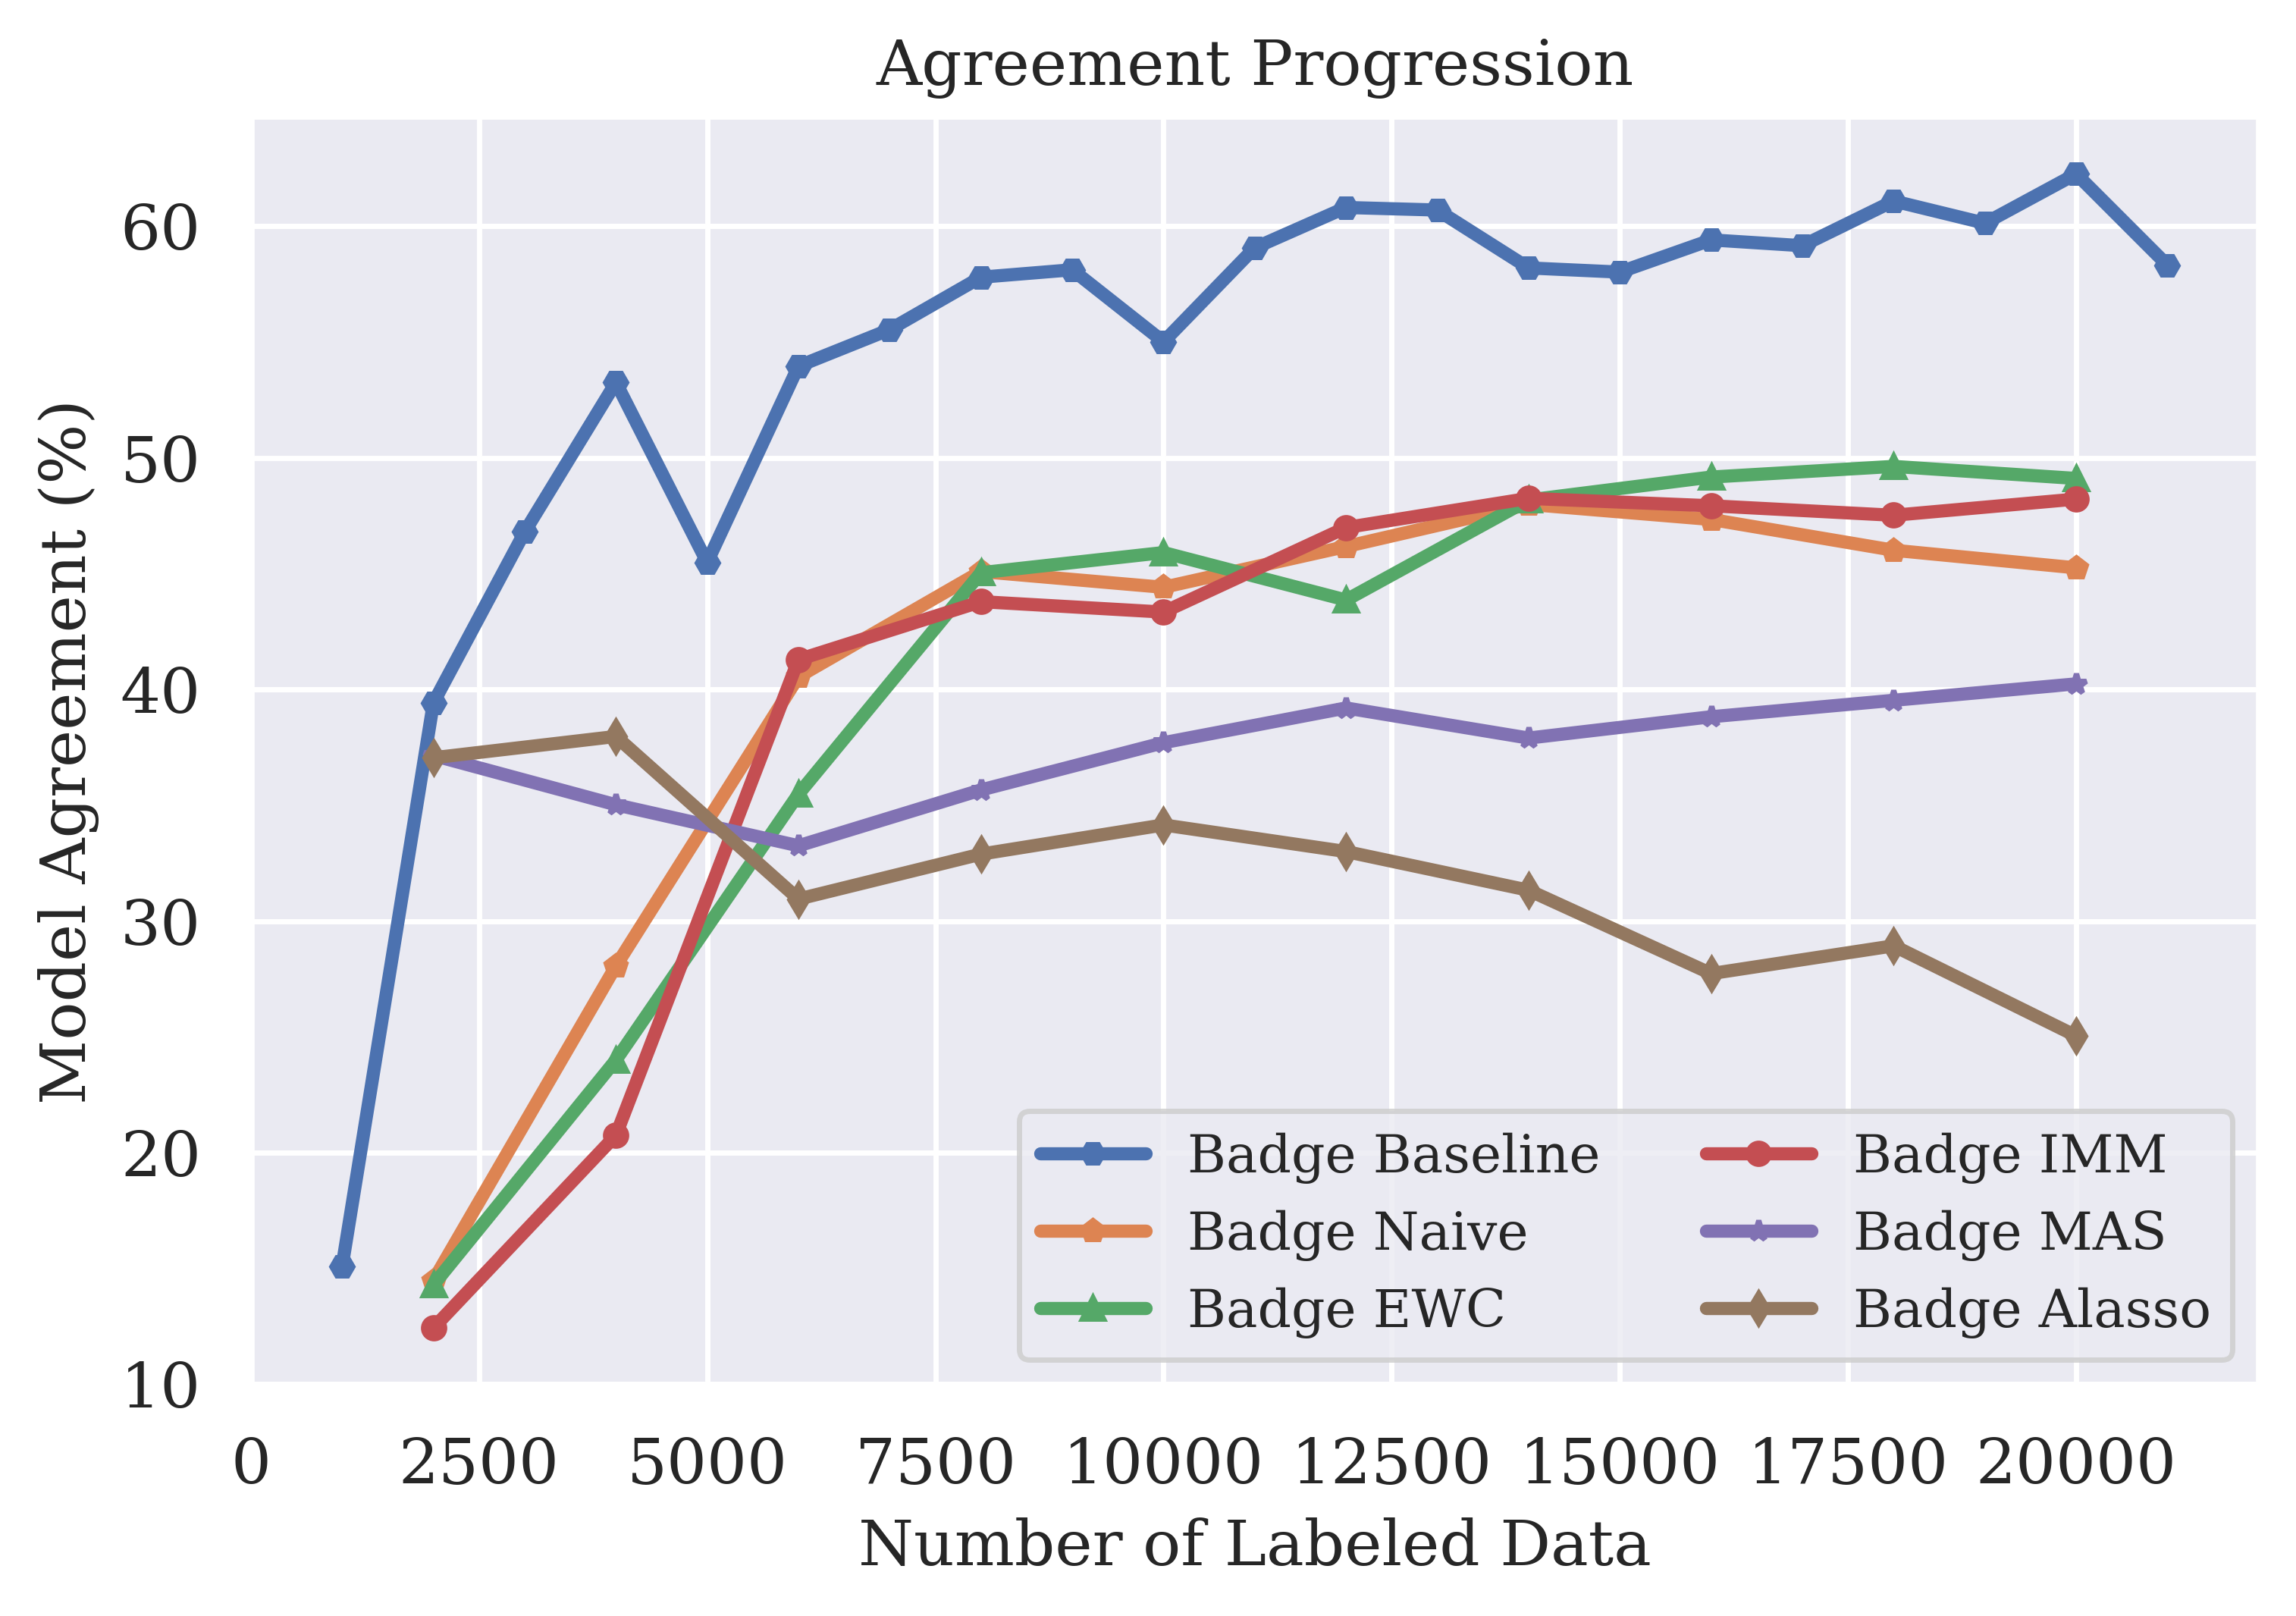
\includegraphics[width=0.5\linewidth]{images/results_CALMS/cifar_label_badge.png}
    \caption{Agreement Comparison for Model Stealing on CIFAR-10 using the predicted class label and the Active Learning strategy \gls{badge}}
    \label{fig:CALMSCIFAR10LabelBadge}
\end{figure}

%Softmax
\begin{figure}[!htb]
    \centering
    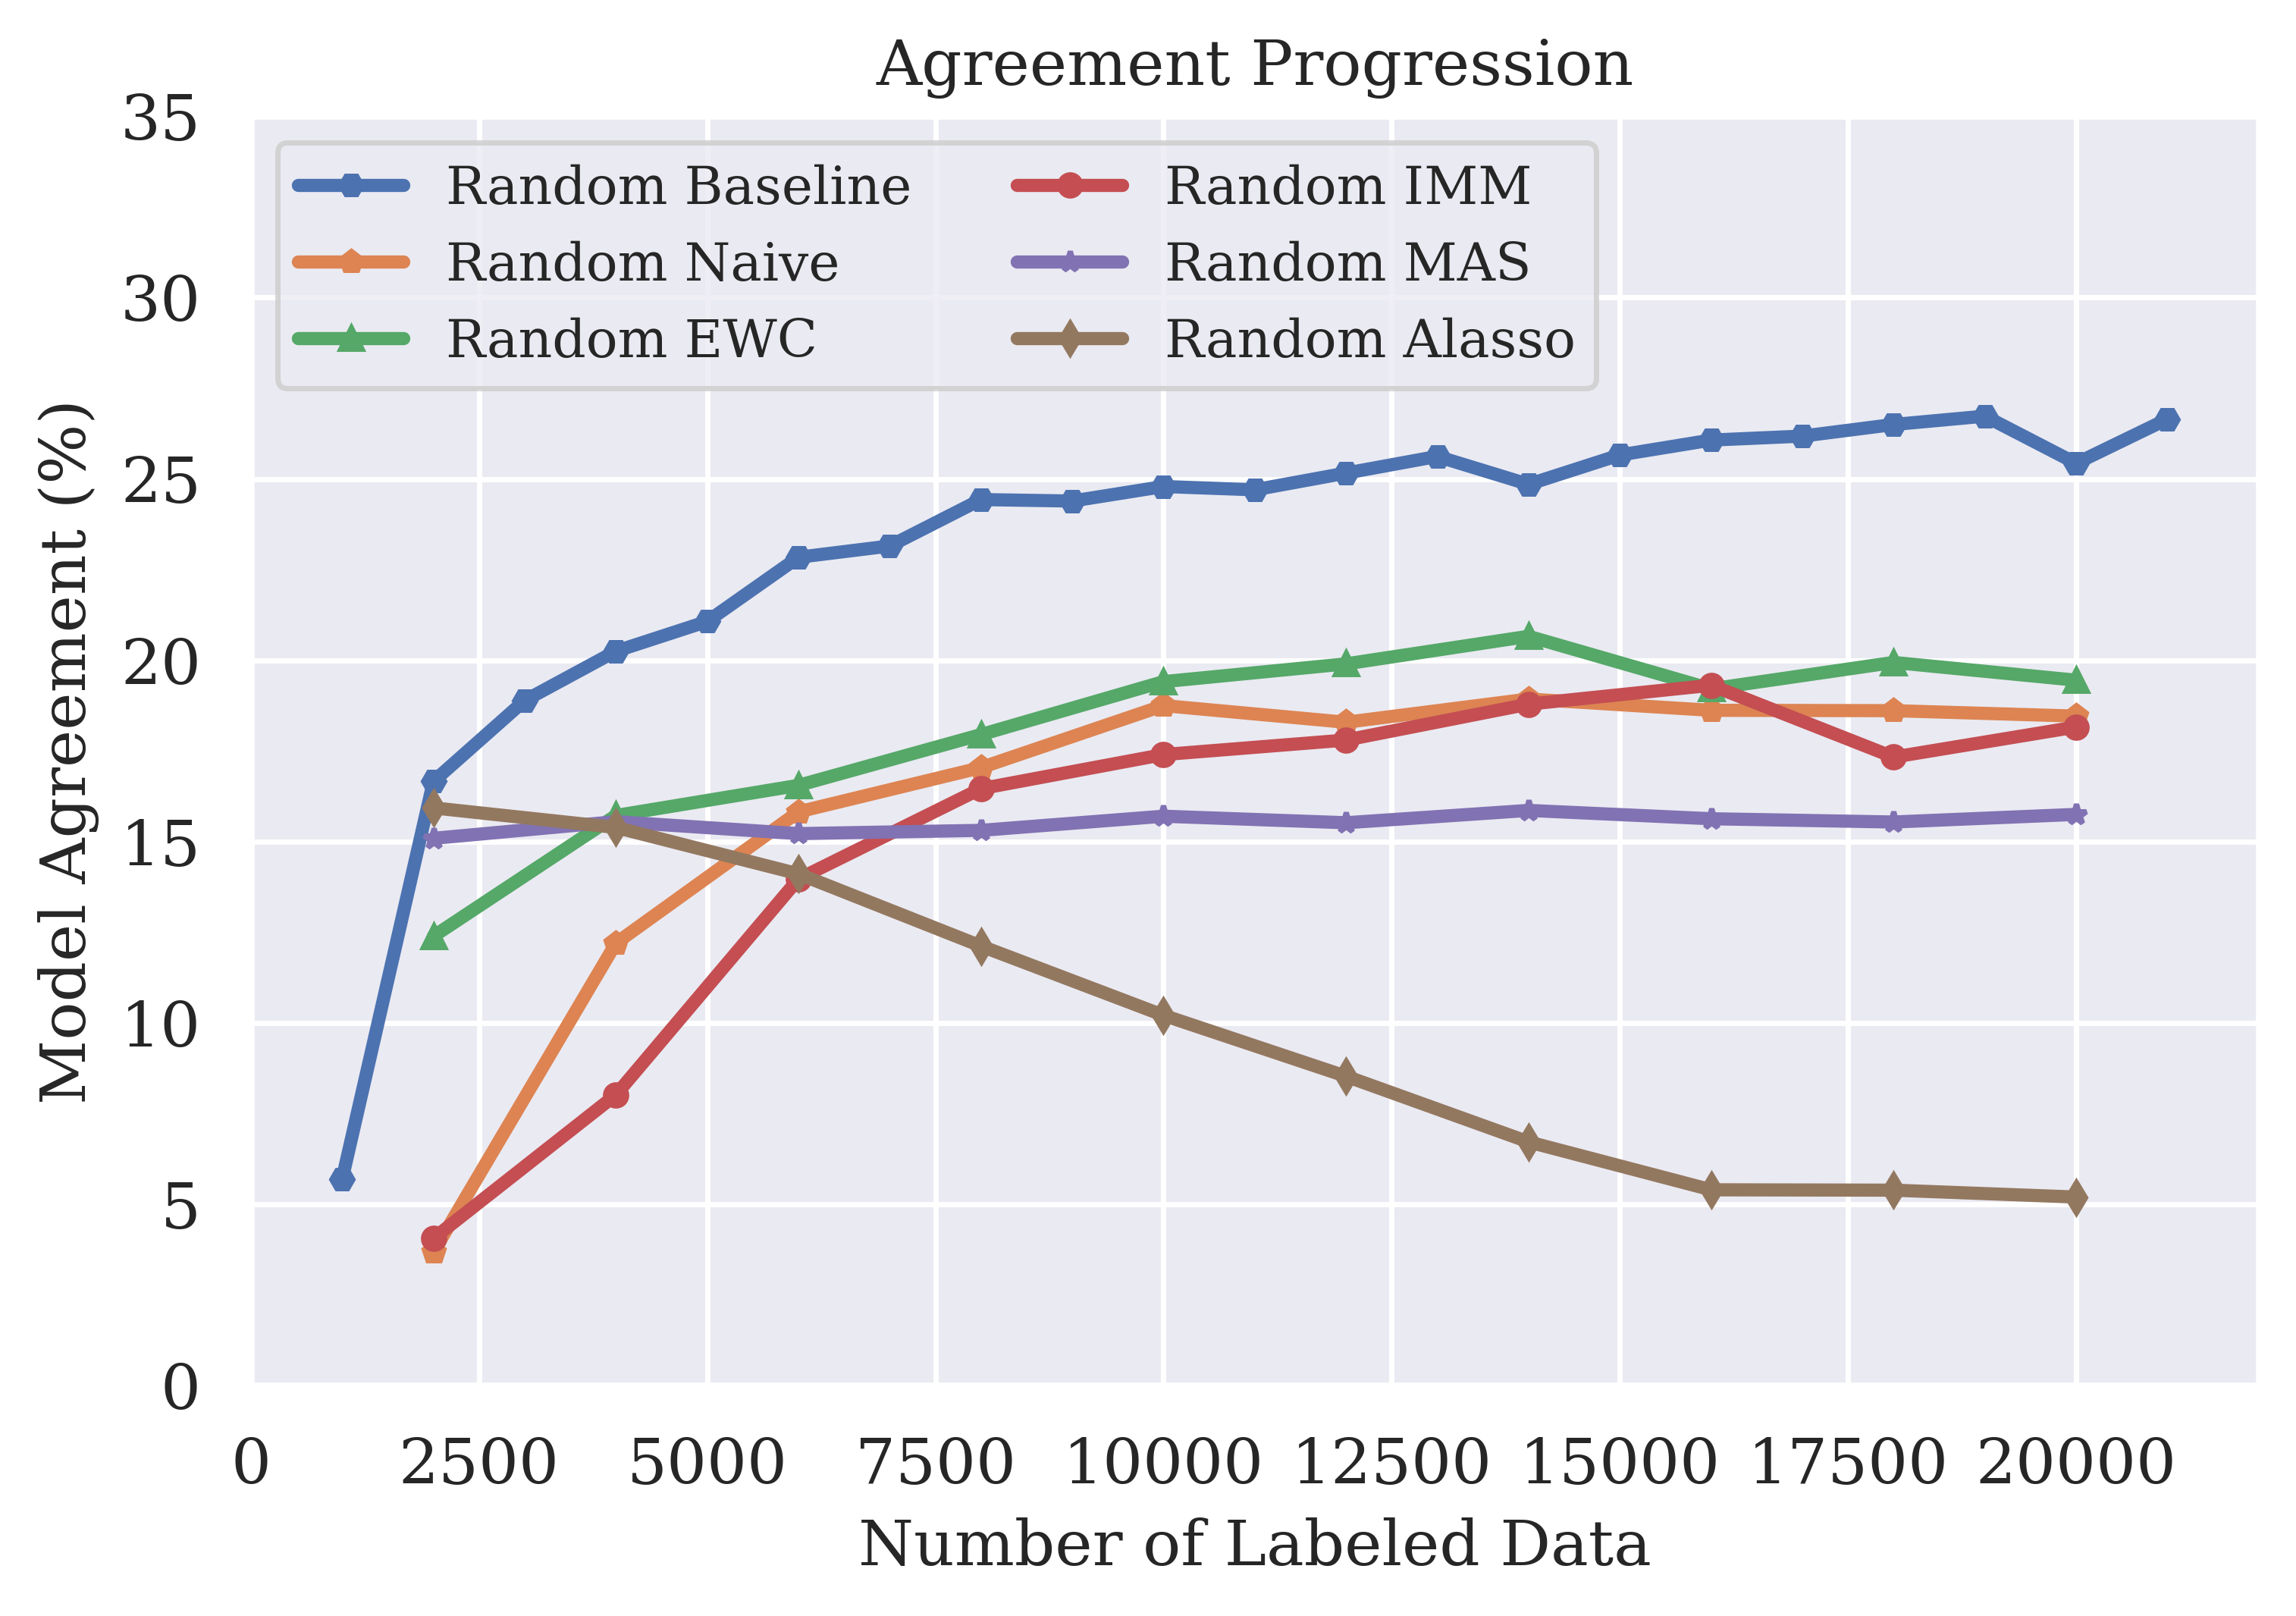
\includegraphics[width=0.5\linewidth]{images/results_CALMS/cifar100_softmax_random.png}
    \caption{Agreement Comparison for Model Stealing on CIFAR-10 using the softmax output and the Active Learning strategy Random}
    \label{fig:CALMSCIFAR10SoftmaxRandom}
\end{figure}

\begin{figure}[!htb]
    \centering
    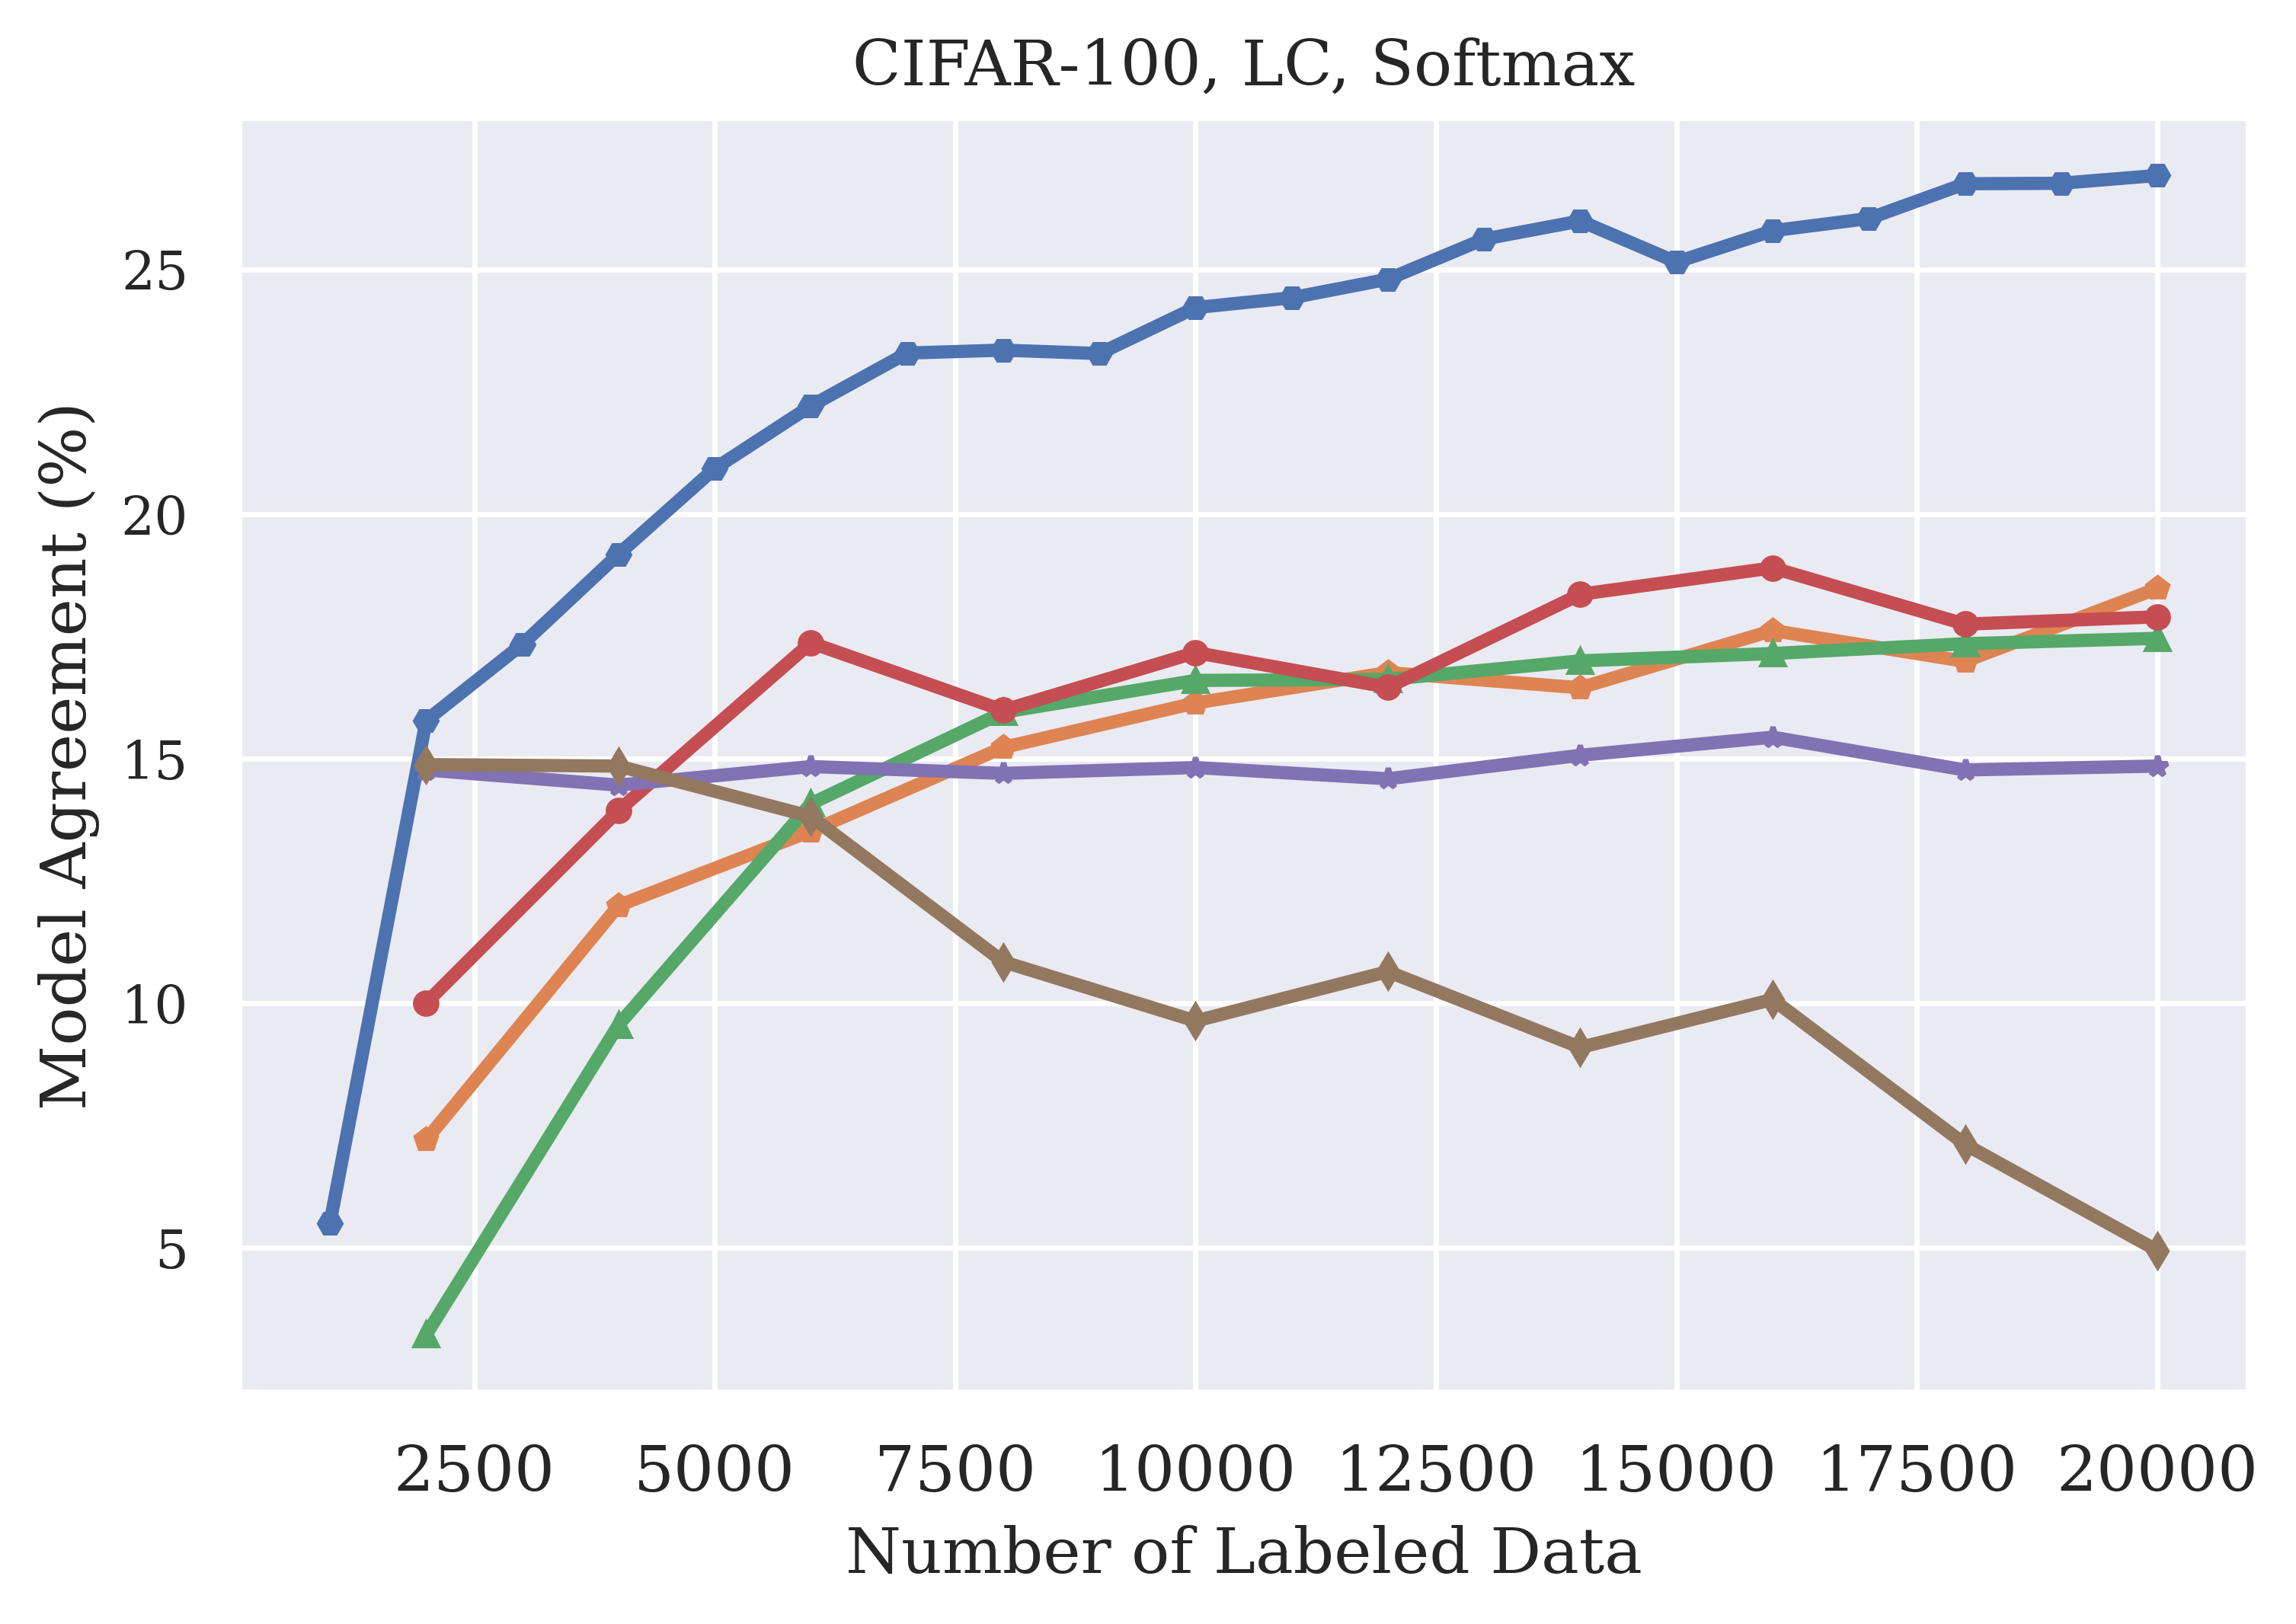
\includegraphics[width=0.5\linewidth]{images/results_CALMS/cifar100_softmax_lc.png}
    \caption{Agreement Comparison for Model Stealing on CIFAR10 using the softmax output and the Active Learning strategy \gls{lc}}
    \label{fig:CALMSCIFAR10SoftmaxLC}
\end{figure}

\begin{figure}[!htb]
    \centering
    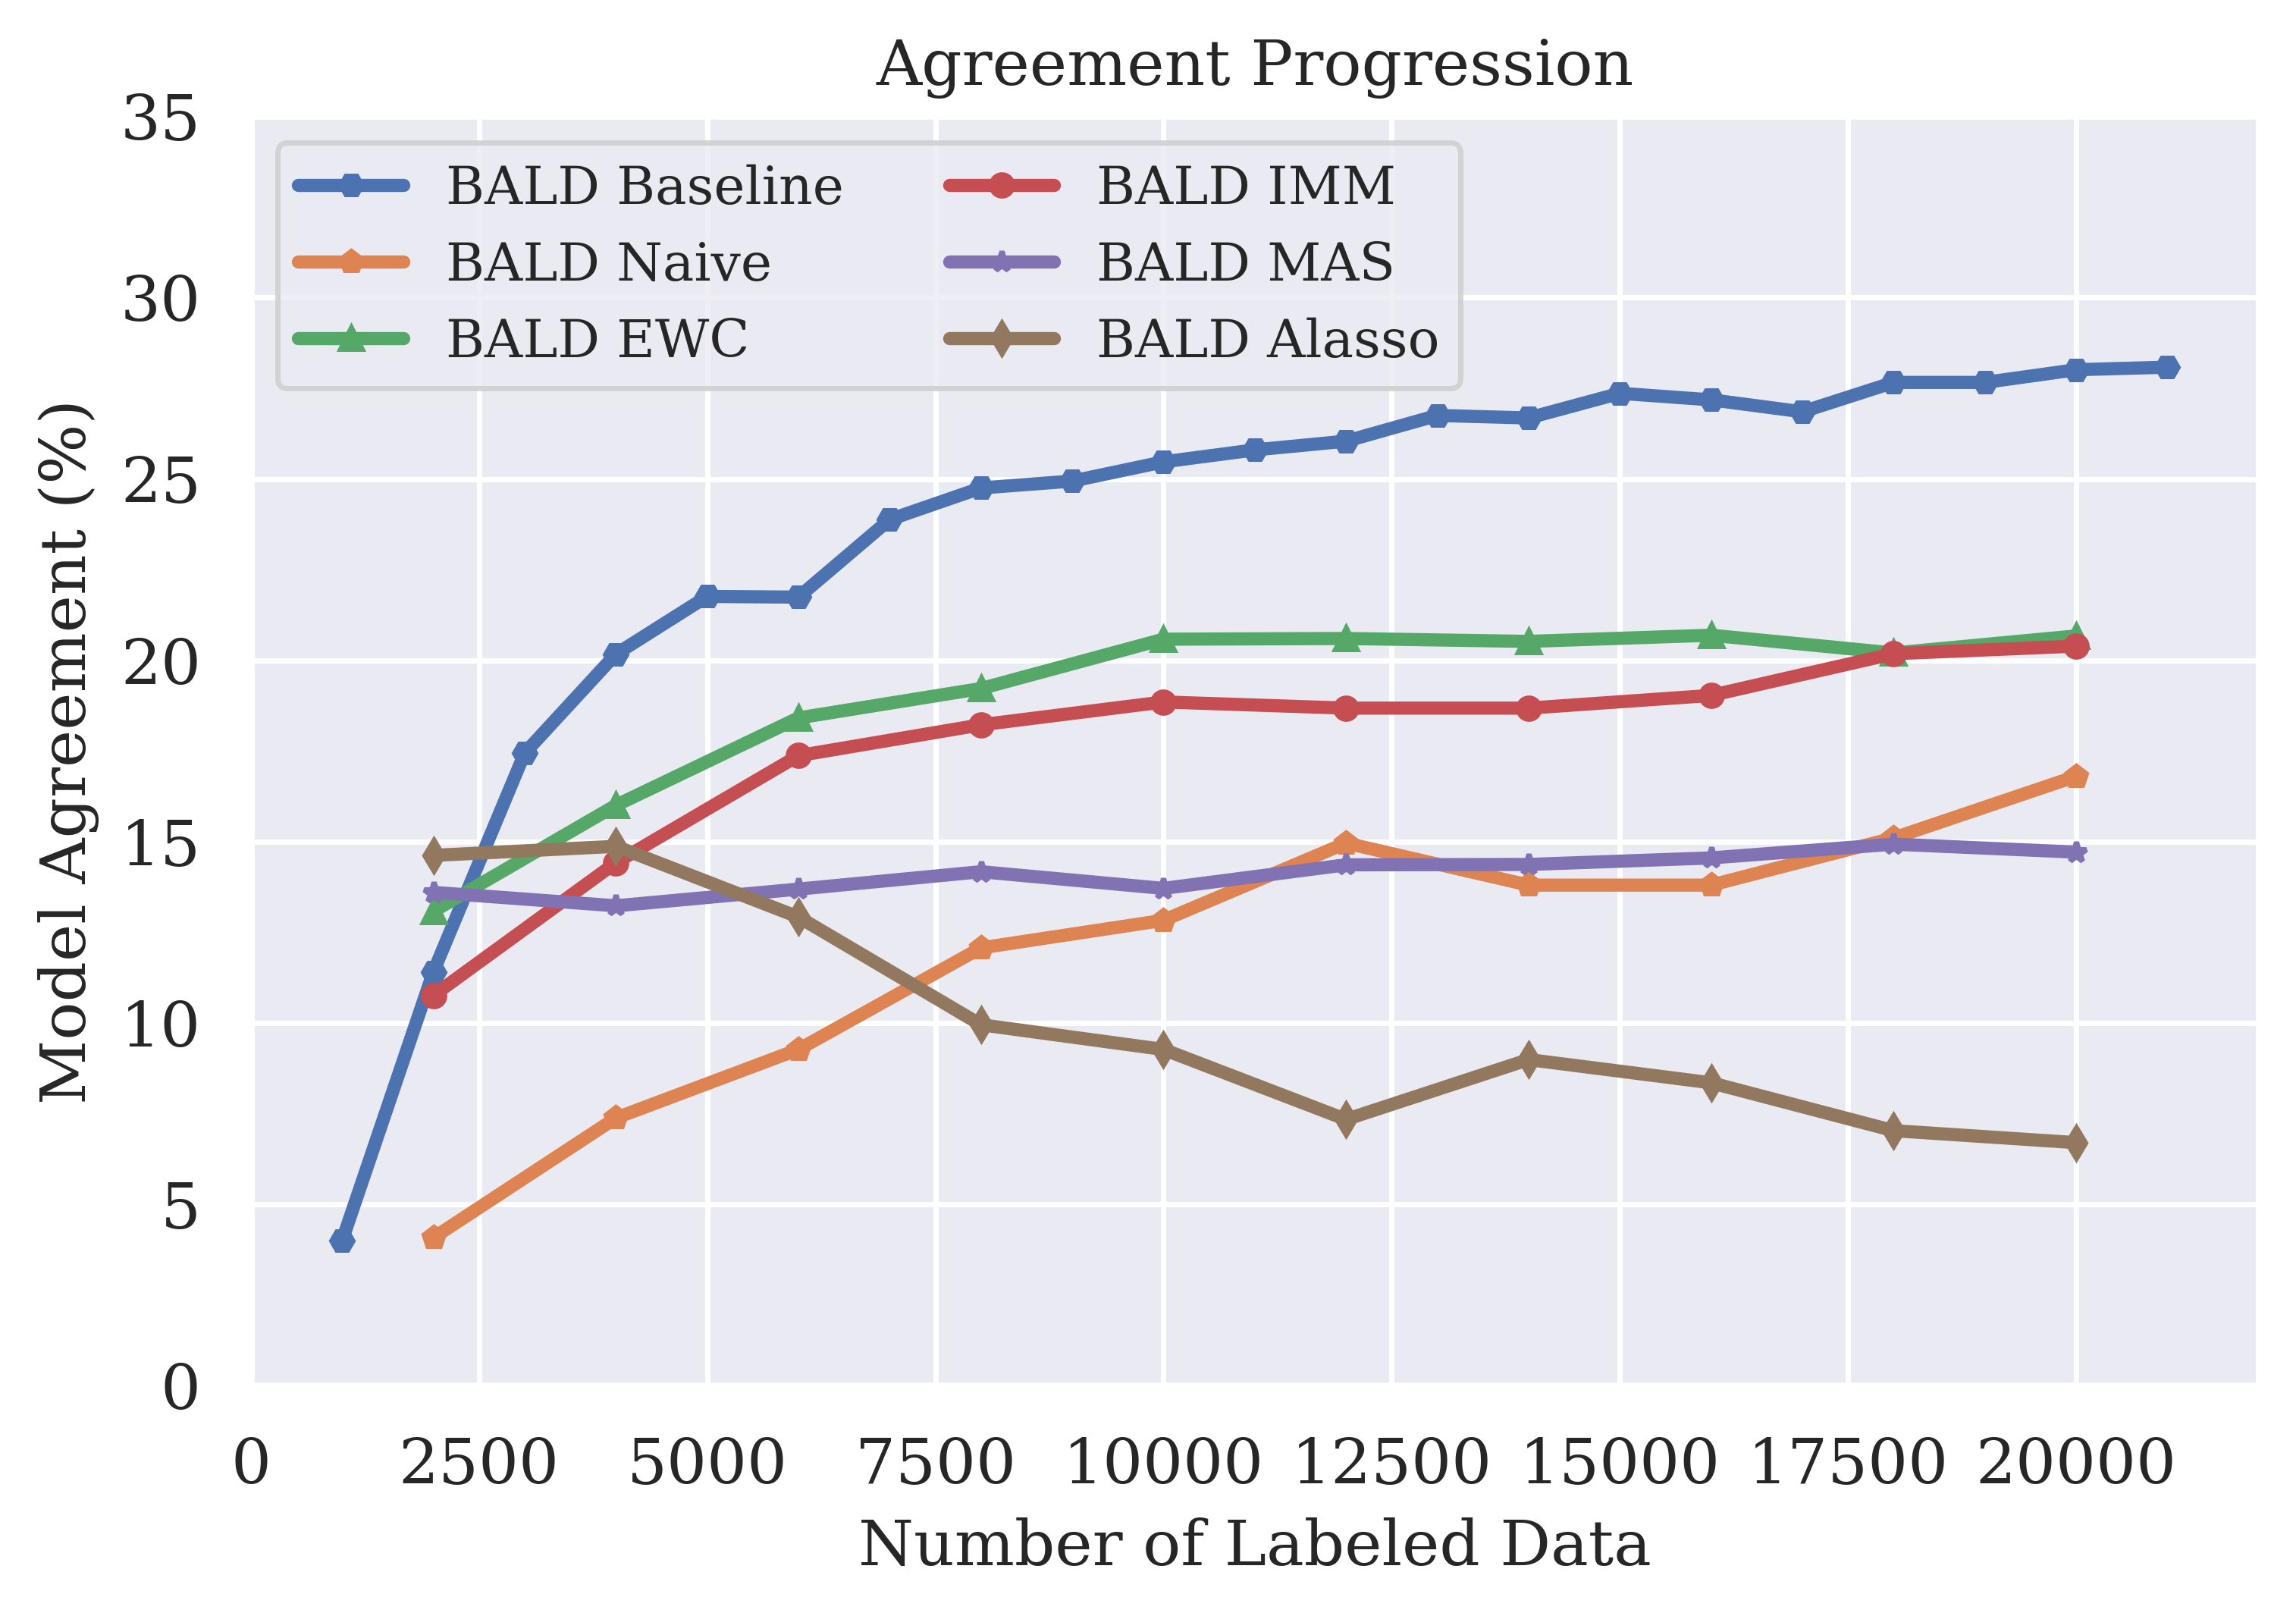
\includegraphics[width=0.5\linewidth]{images/results_CALMS/cifar100_softmax_bald.png}
    \caption{Agreement Comparison for Model Stealing on CIFAR-10 using the softmax output and the Active Learning strategy \gls{bald}}
    \label{fig:CALMSCIFAR10SoftmaxBALD}
\end{figure}

\begin{figure}[!htb]
    \centering
    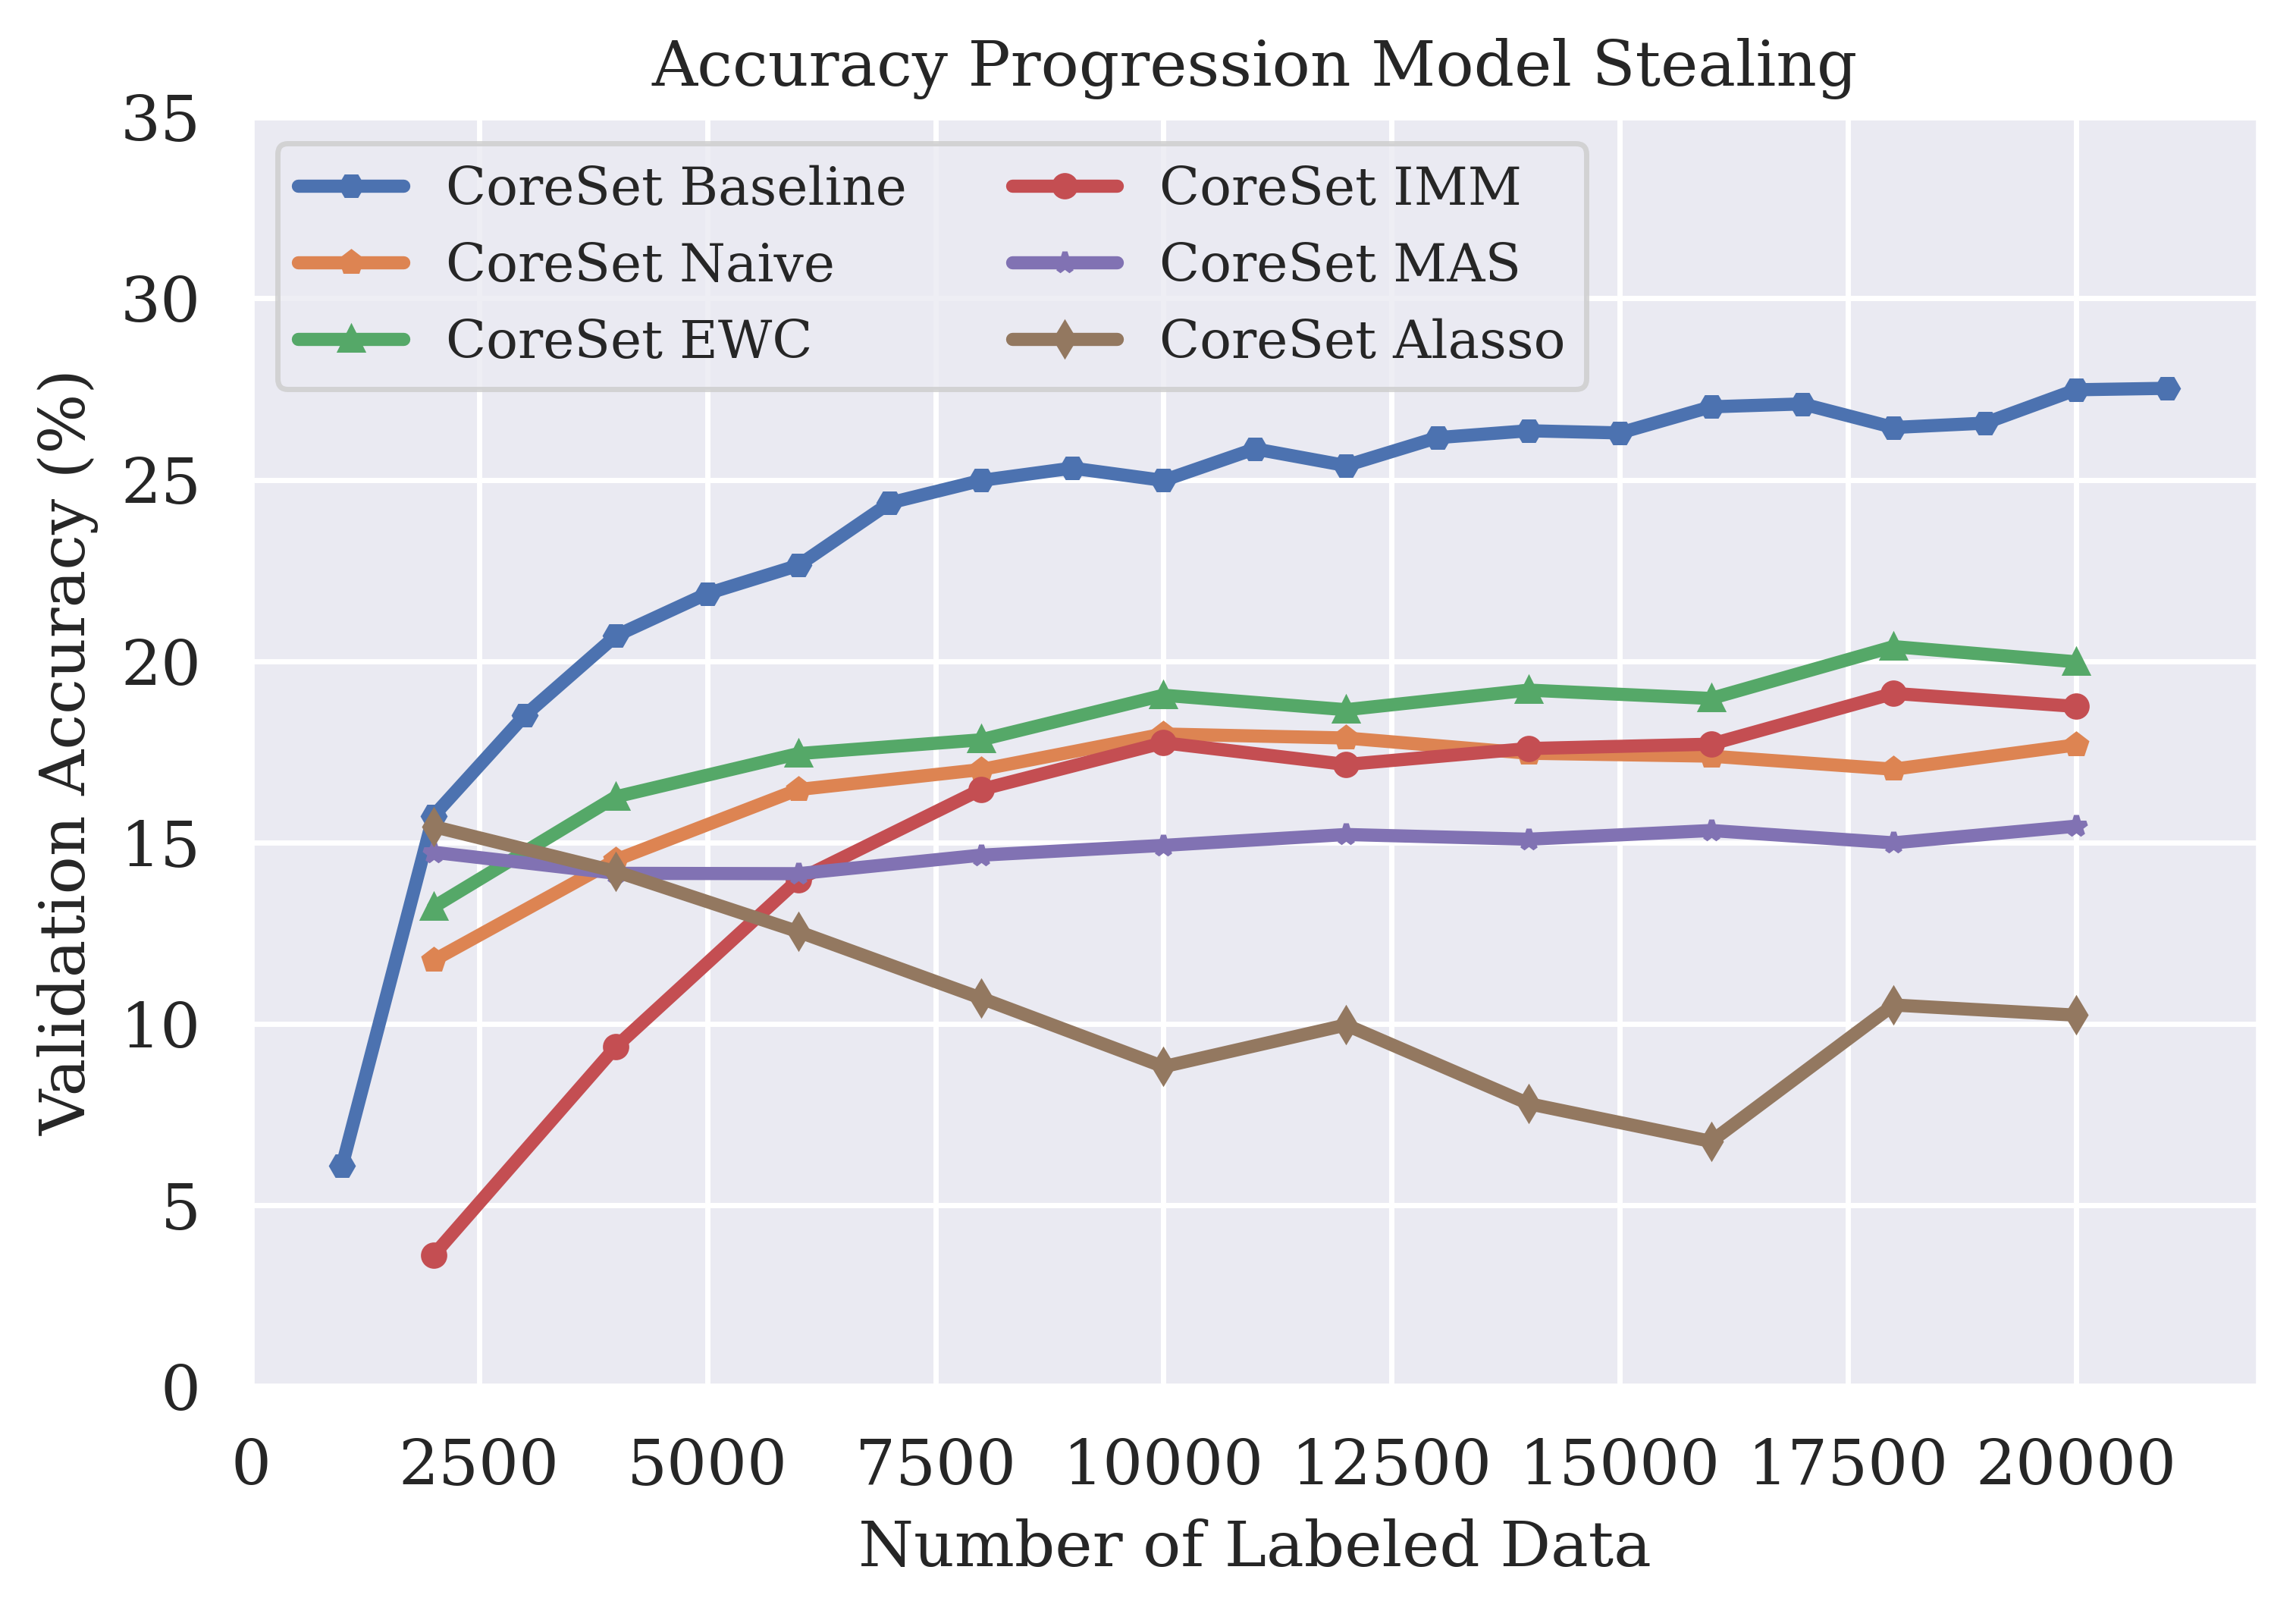
\includegraphics[width=0.5\linewidth]{images/results_CALMS/cifar100_softmax_coreset.png}
    \caption{Agreement Comparison for Model Stealing on CIFAR-10 using the softmax output and the Active Learning strategy CoreSet}
    \label{fig:CALMSCIFAR10SoftmaxCoreSet}
\end{figure}

\begin{figure}[!htb]
    \centering
    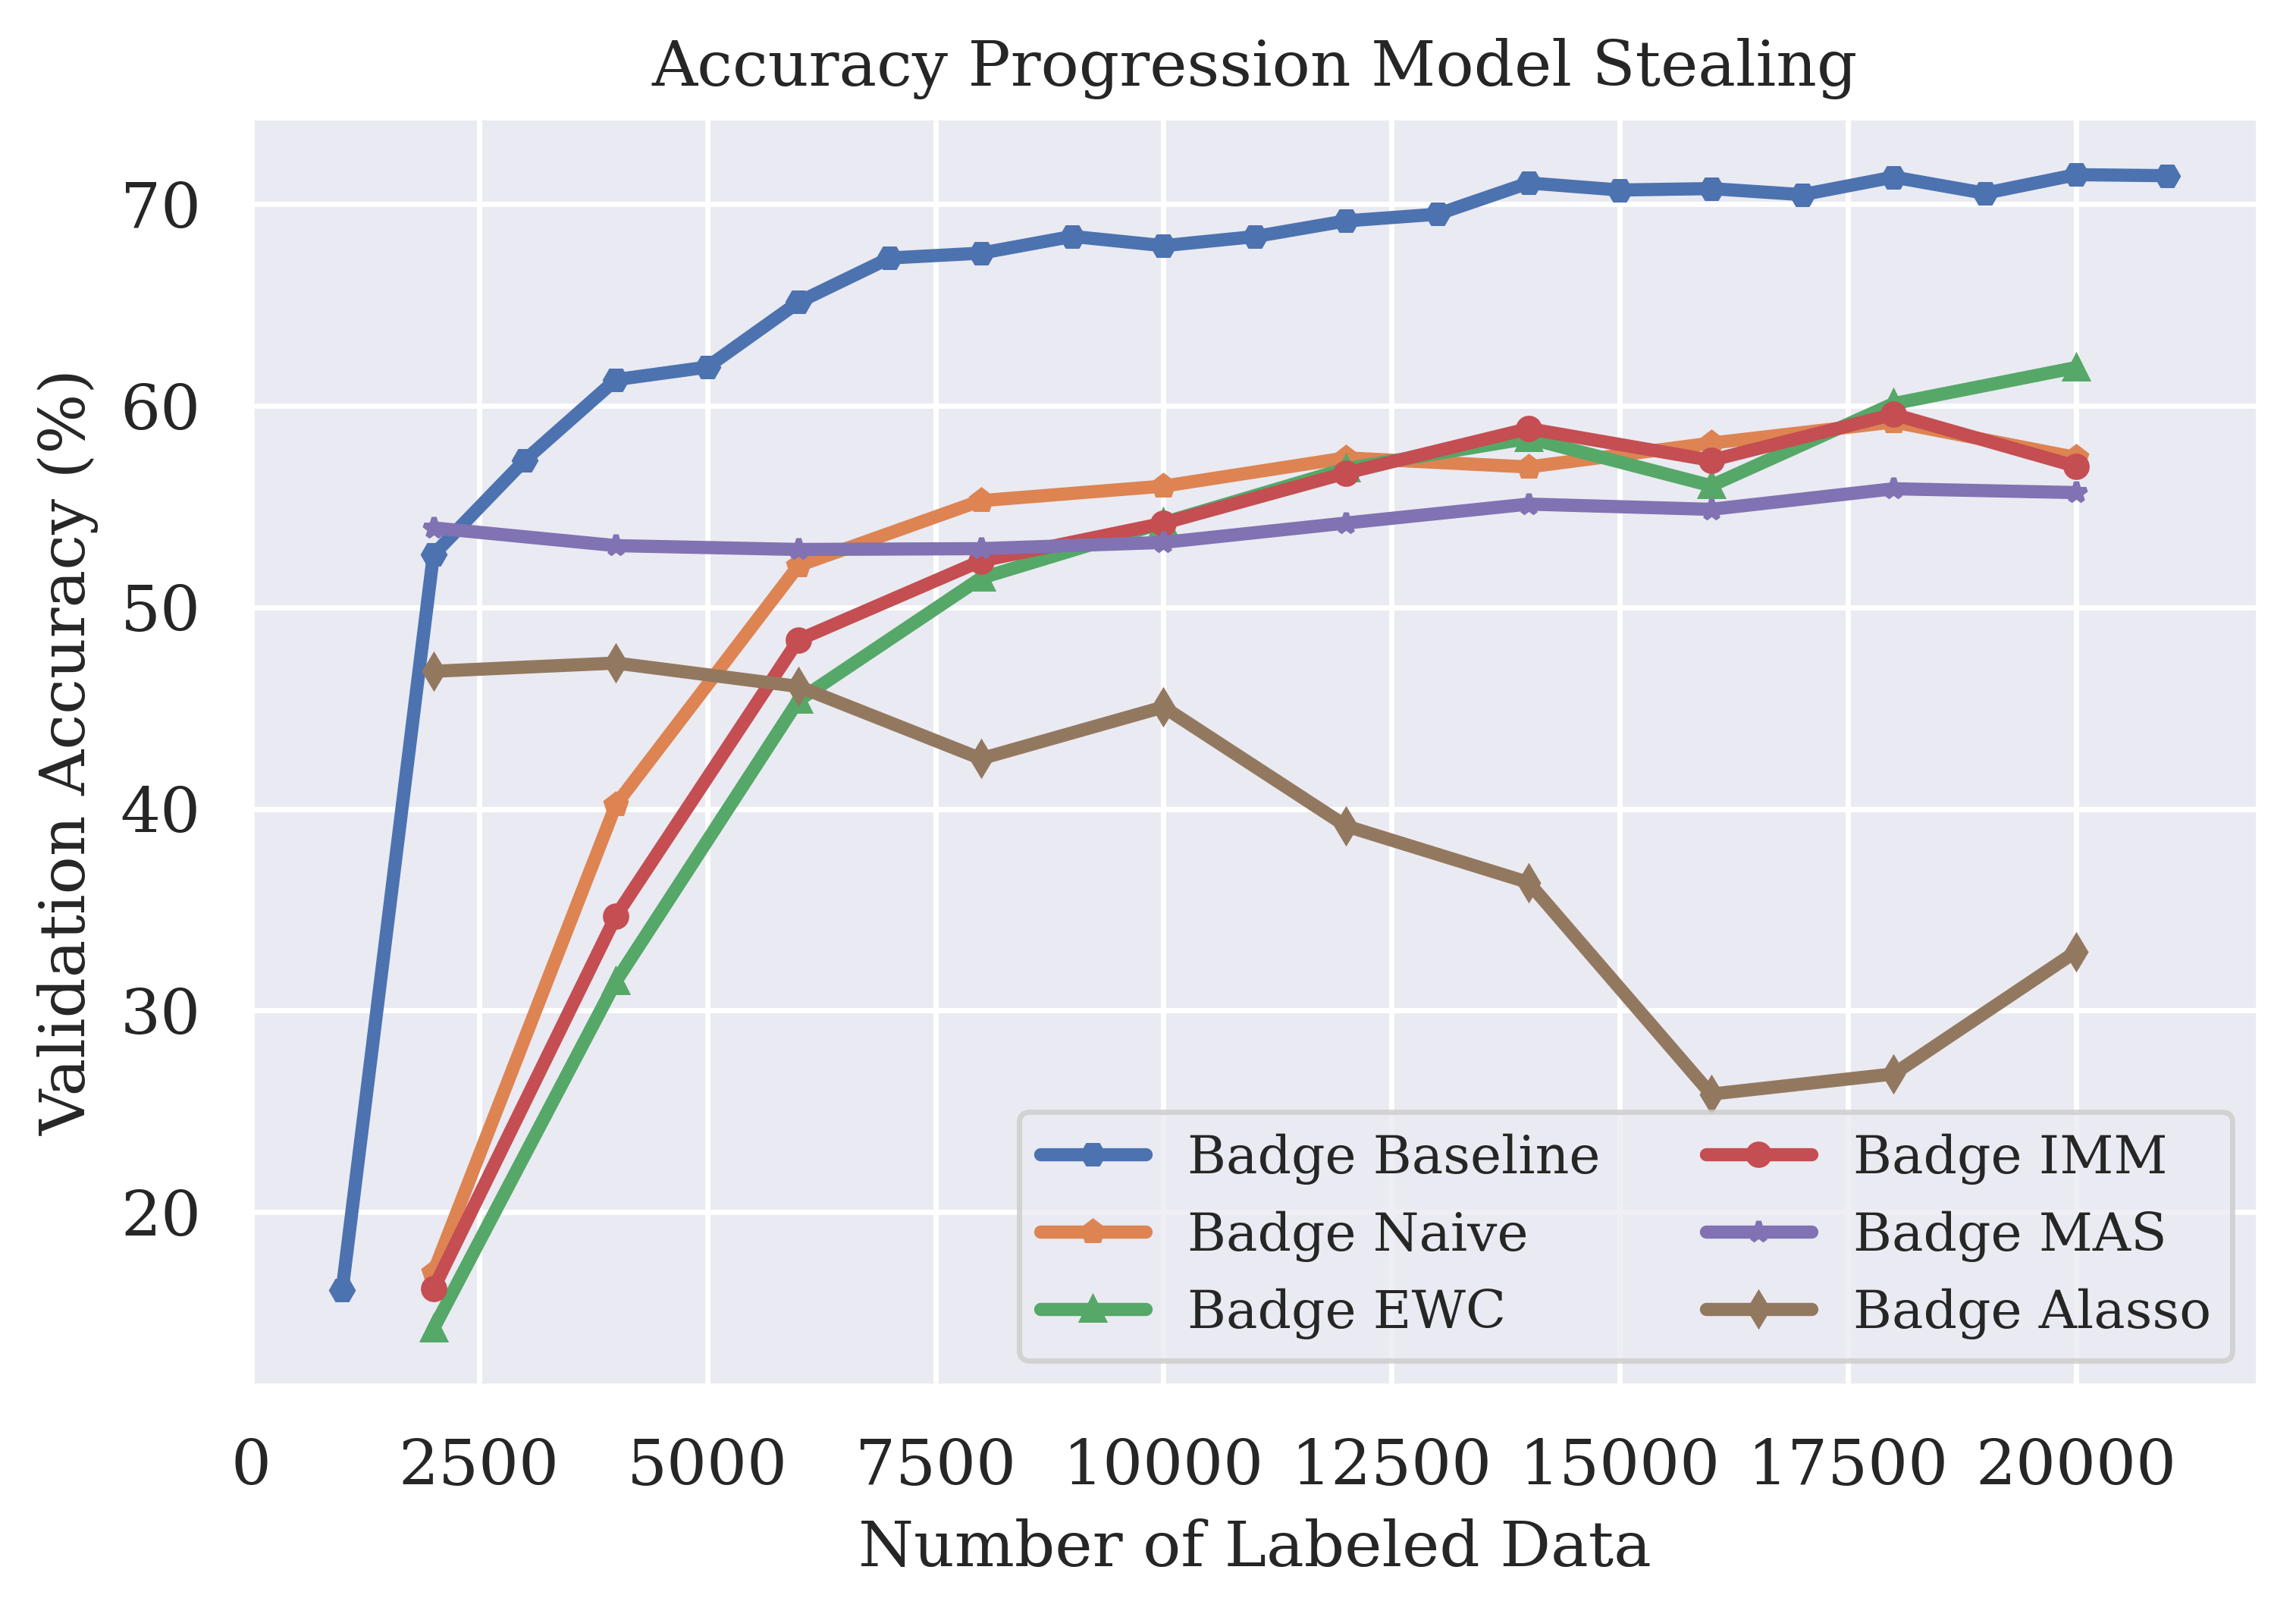
\includegraphics[width=0.5\linewidth]{images/results_CALMS/cifar_softmax_badge.png}
    \caption{Agreement Comparison for Model Stealing on CIFAR-10 using the softmax output and the Active Learning strategy \gls{badge}}
    \label{fig:CALMSCIFAR10SoftmaxBadge}
\end{figure}


\subsubsection{CIFAR-100}
\label{sec:Appendix:CALMS:CIFAR100}
In this section, we present the full runs of all experiments which involve Continual Active Learning using CIFAR-100 as a Target Model Dataset.

\begin{figure}[!htb]
    \centering
    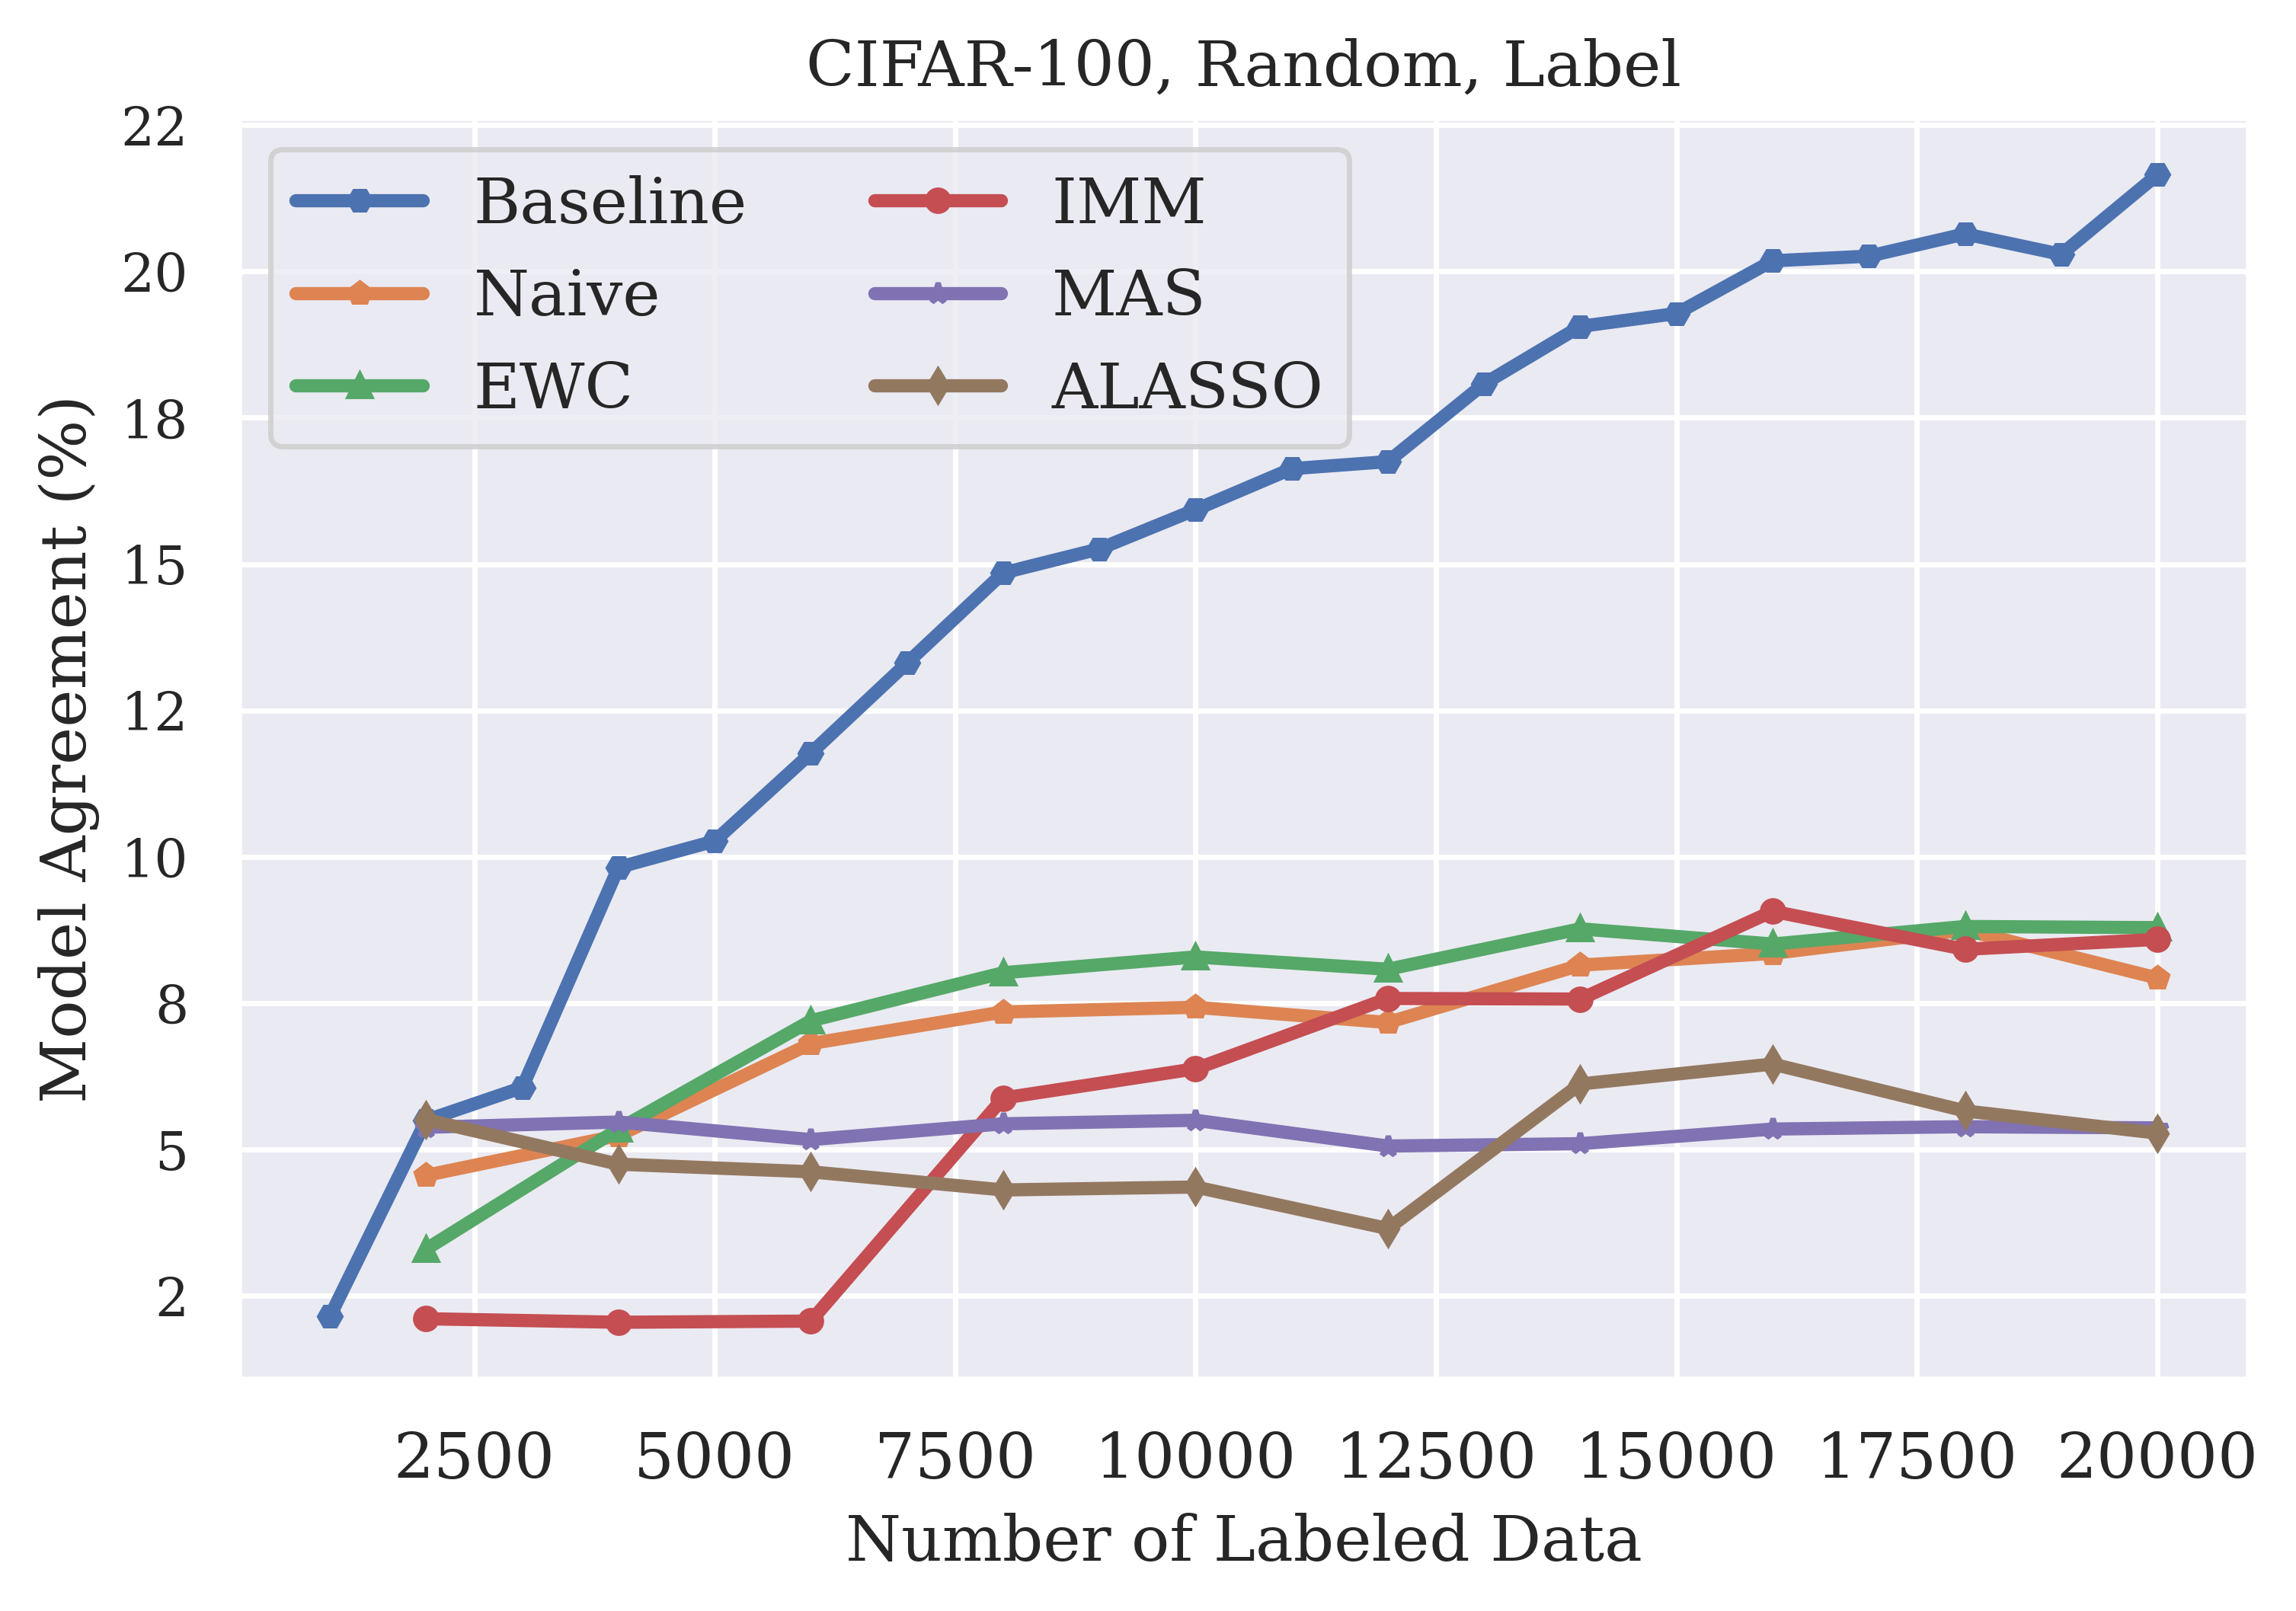
\includegraphics[width=0.5\linewidth]{images/results_CALMS/cifar100_label_random.png}
    \caption{Agreement Comparison for Model Stealing on CIFAR-100 using the predicted class label and the Active Learning strategy Random}
    \label{fig:CALMSCIFAR100LabelRandom}
\end{figure}

\begin{figure}[!htb]
    \centering
    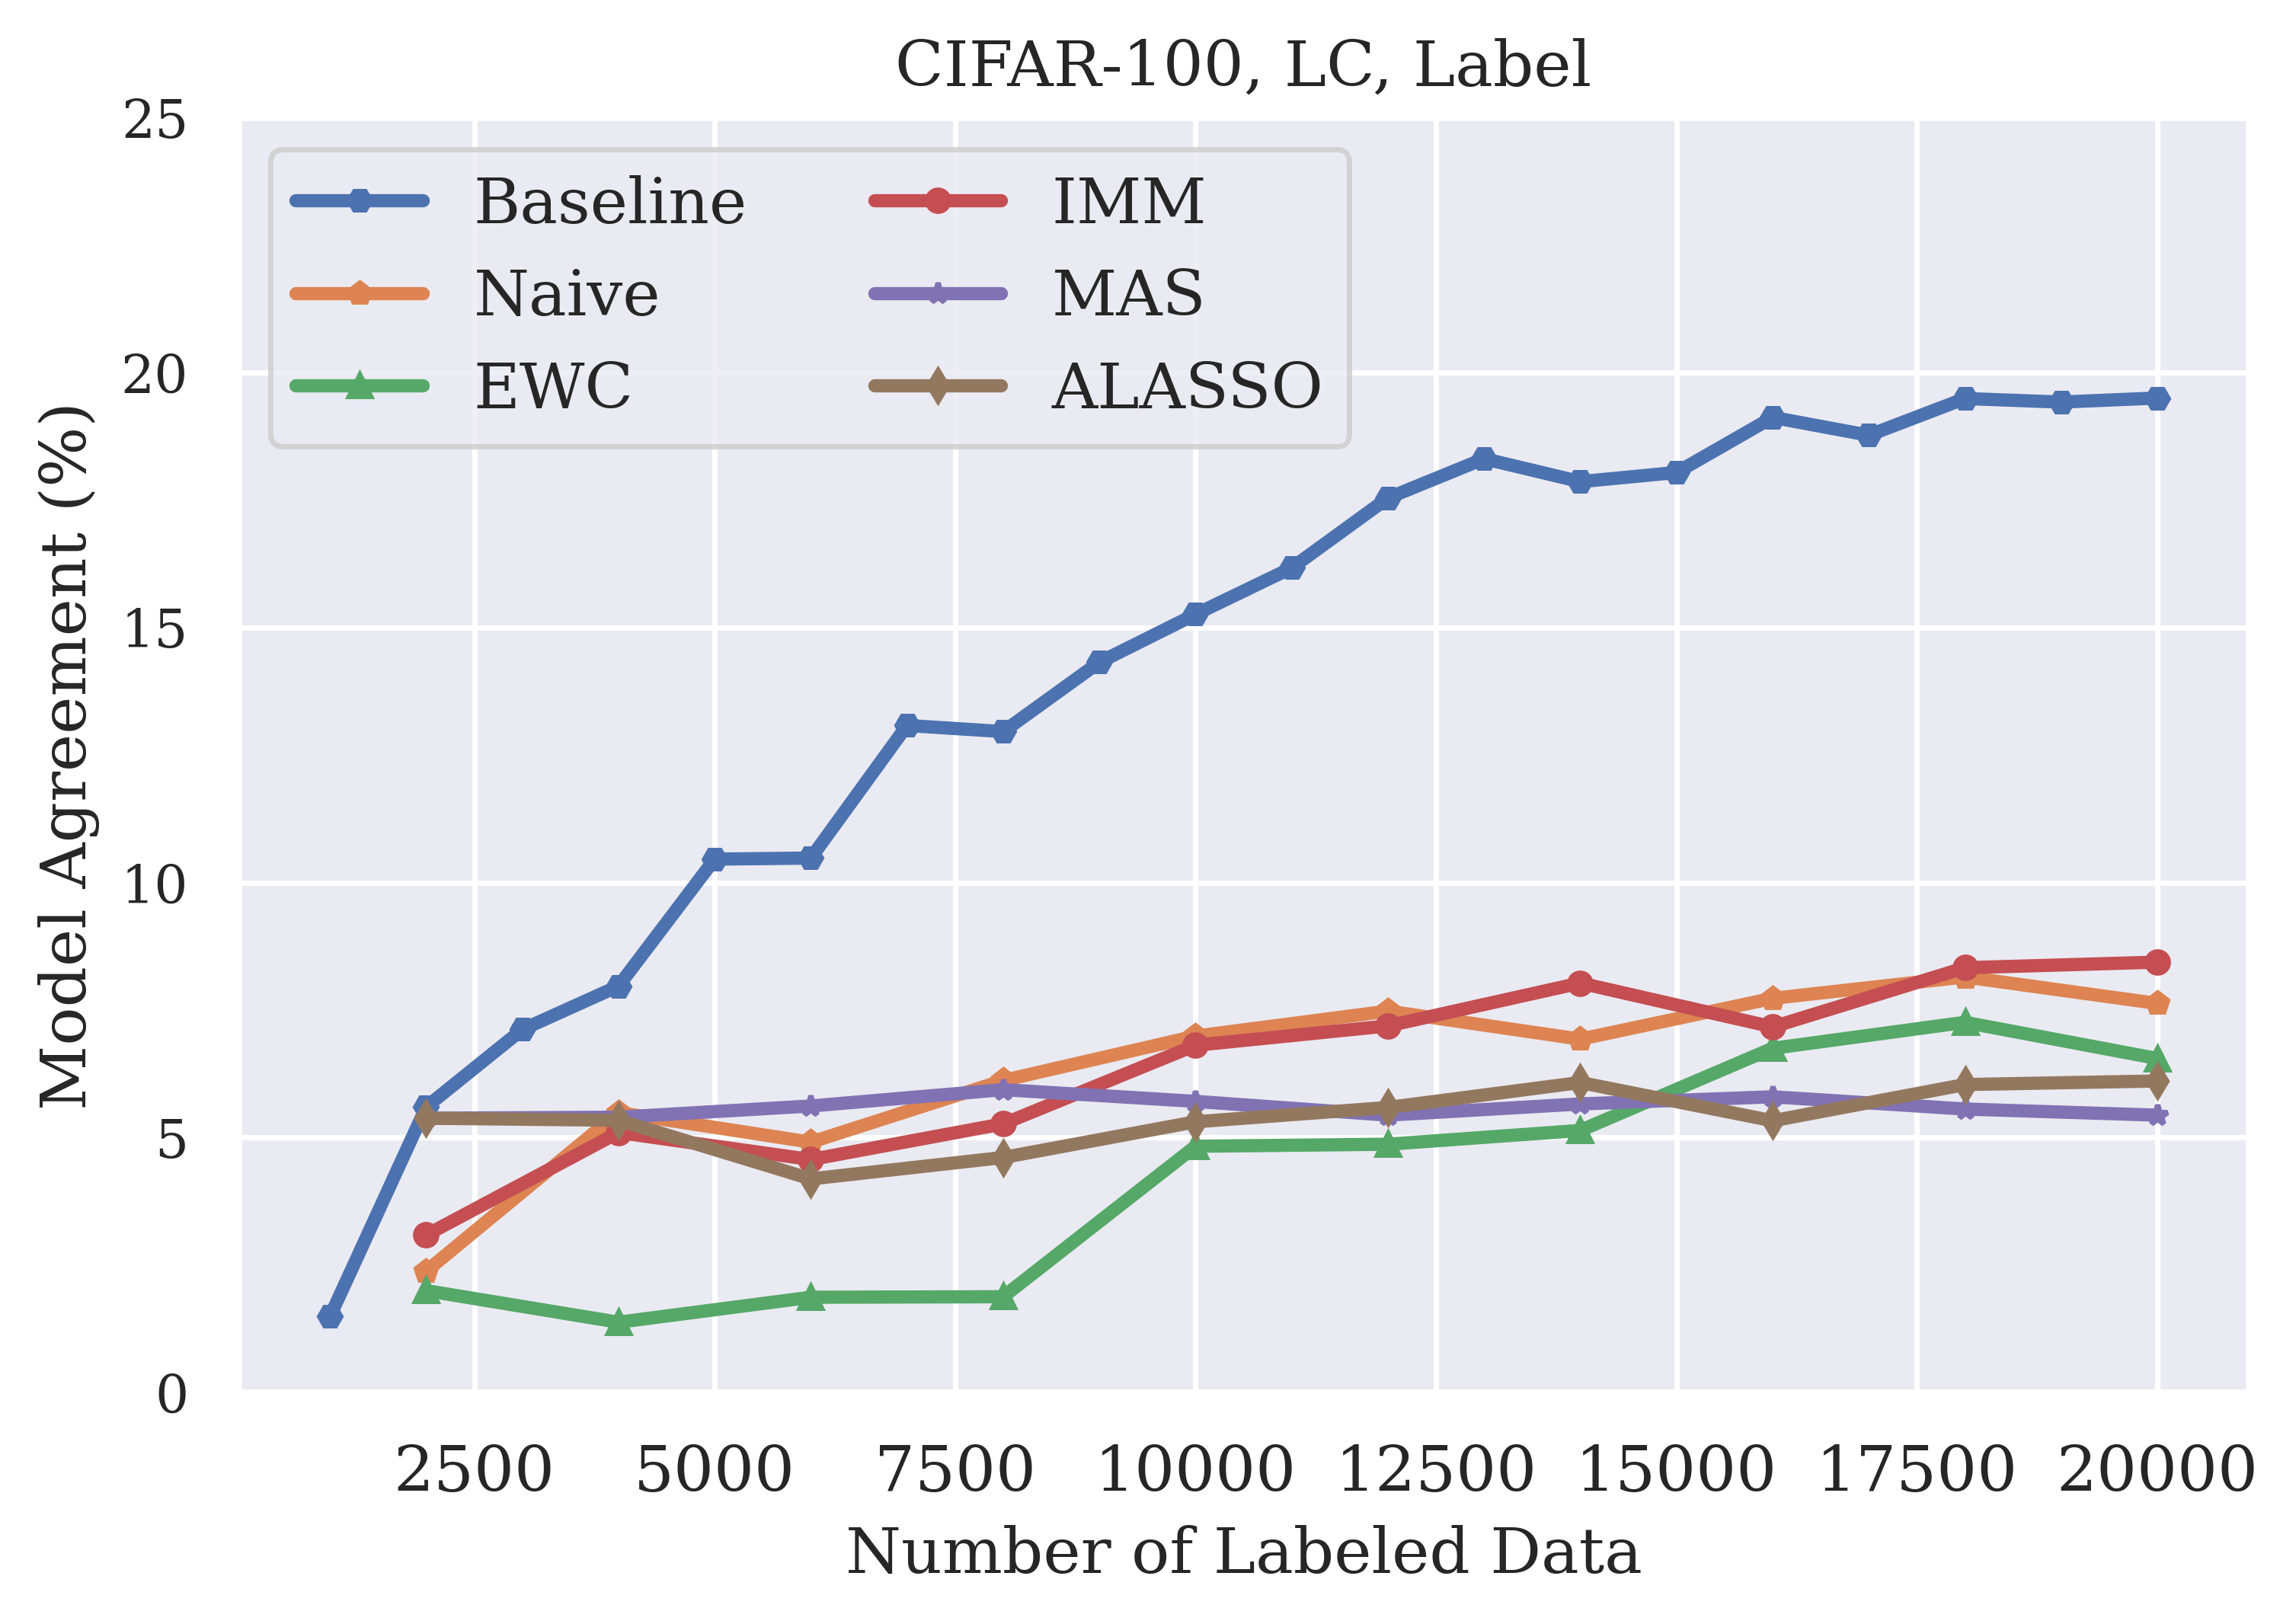
\includegraphics[width=0.5\linewidth]{images/results_CALMS/cifar100_label_lc.png}
    \caption{Agreement Comparison for Model Stealing on CIFAR-100 using the predicted class label and the Active Learning strategy \gls{lc}}
    \label{fig:CALMSCIFAR100LabelLC}
\end{figure}

\begin{figure}[!htb]
    \centering
    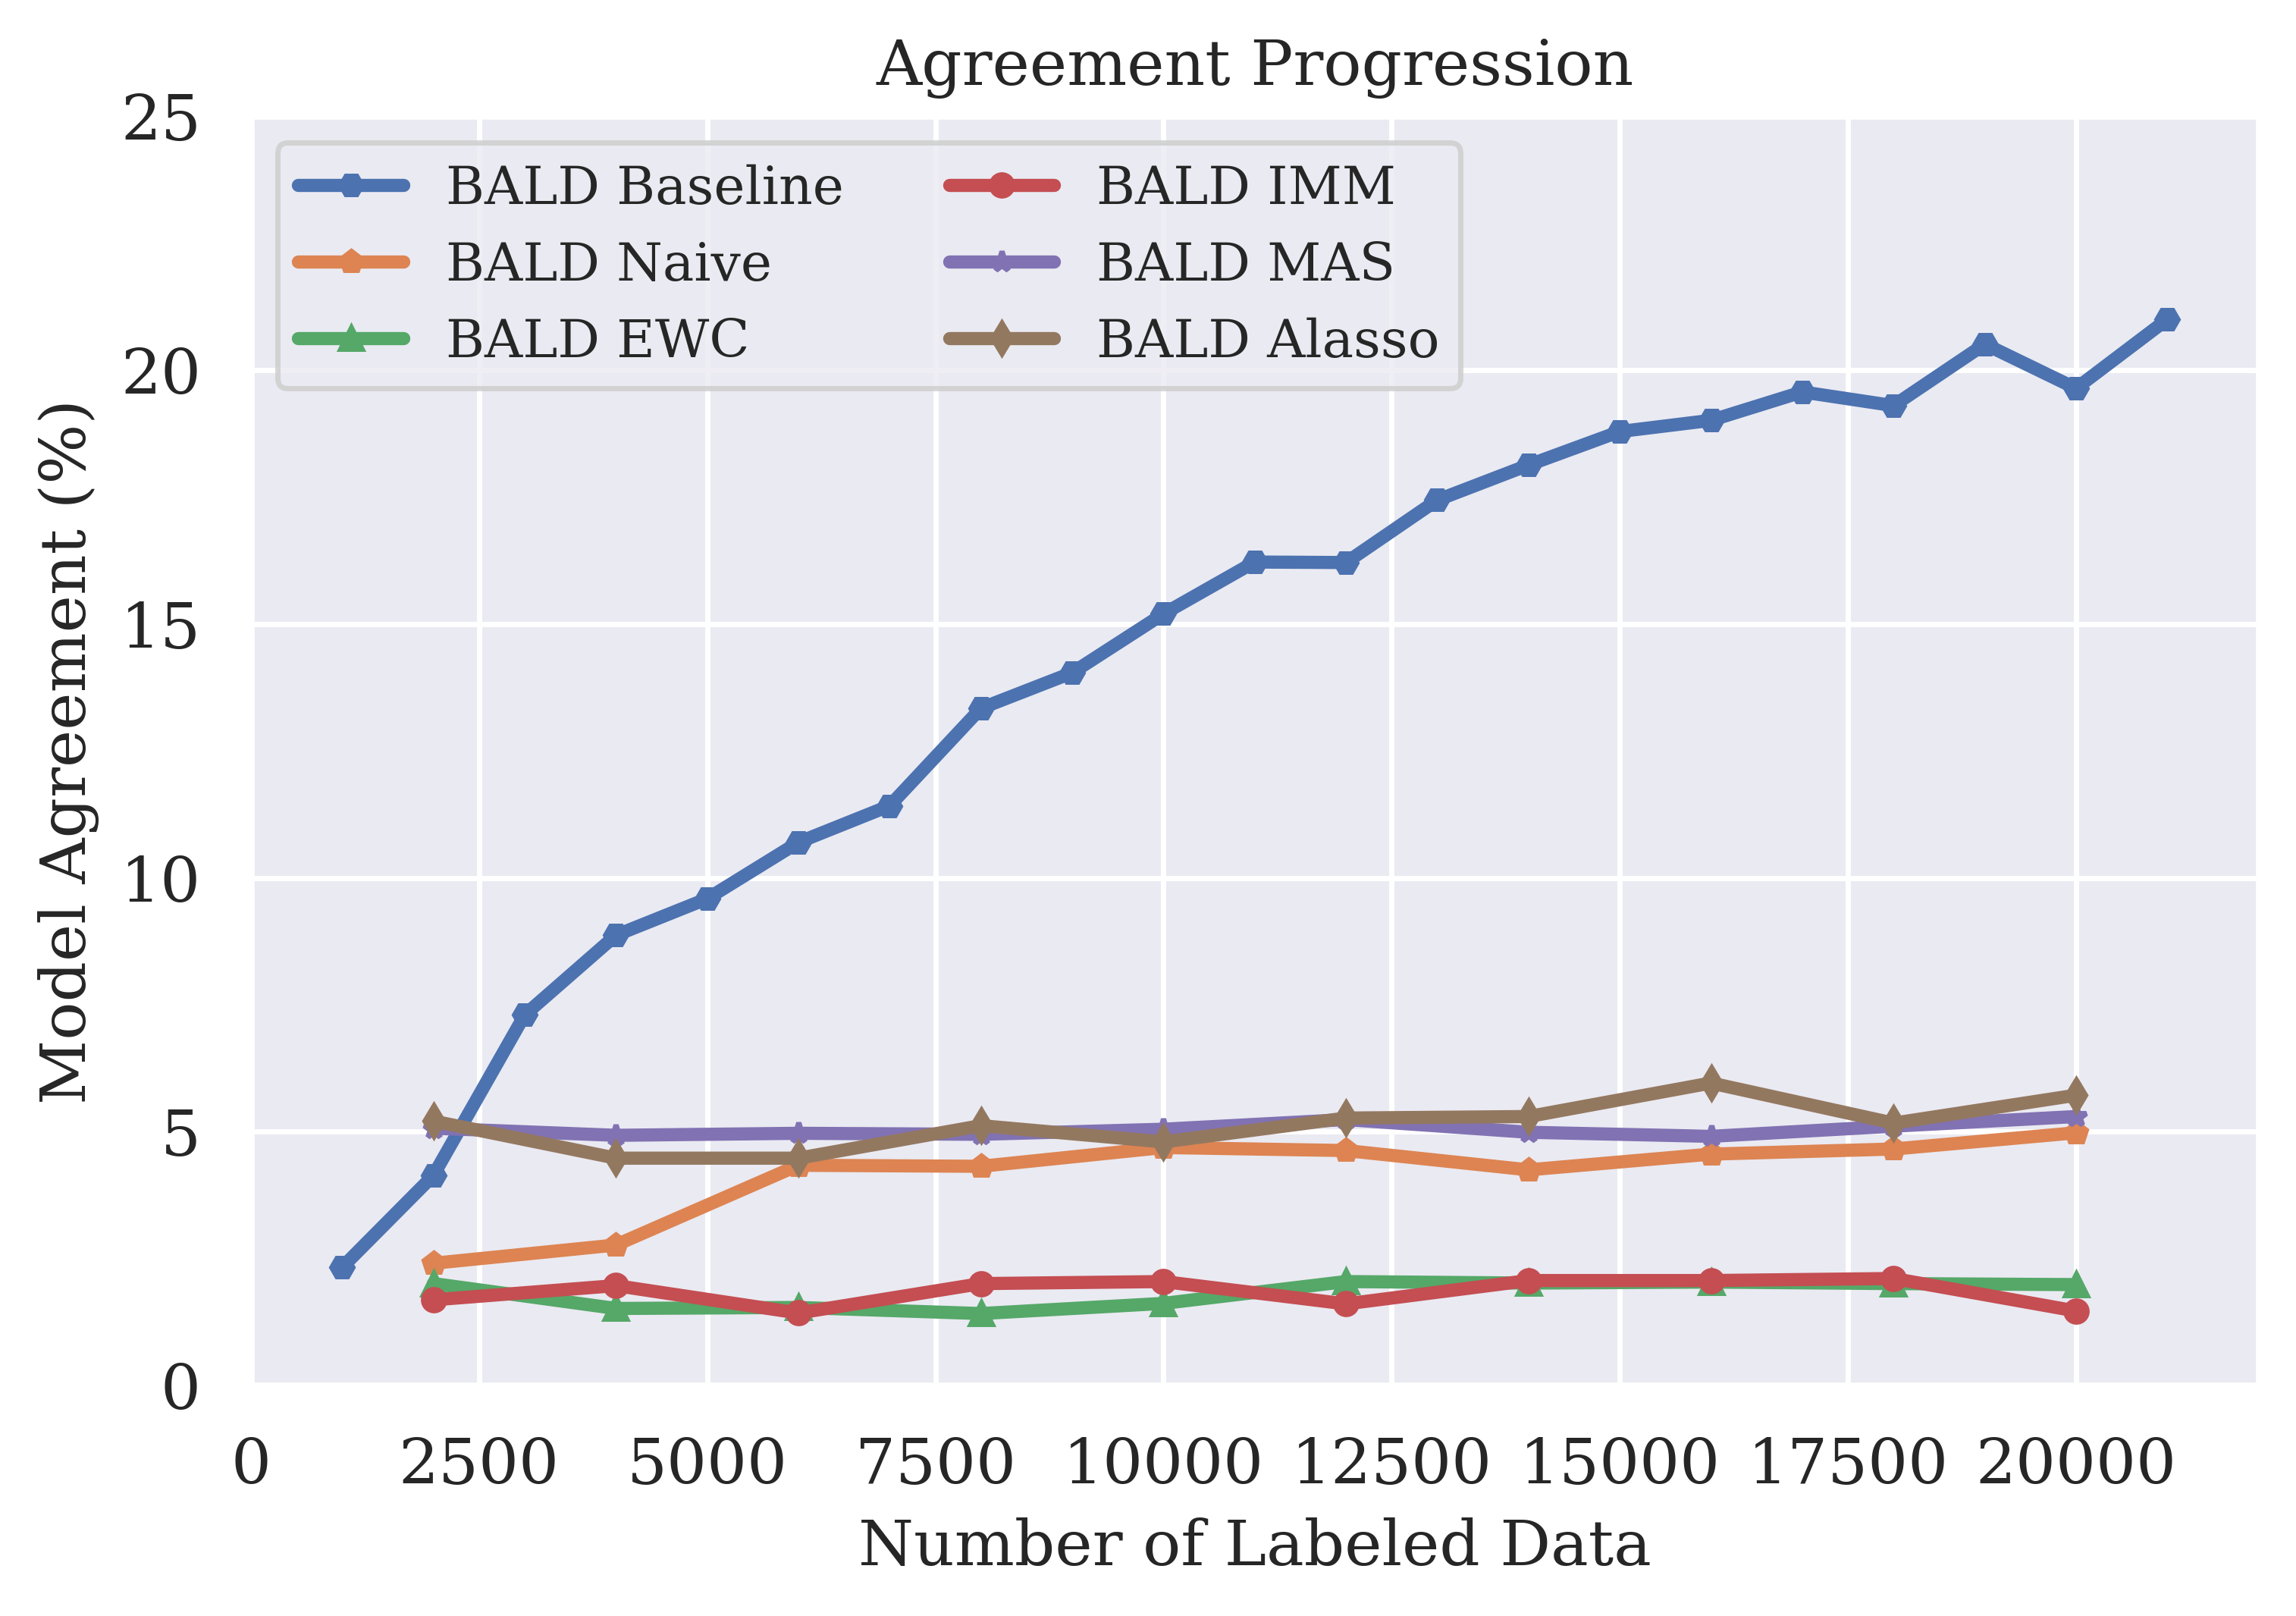
\includegraphics[width=0.5\linewidth]{images/results_CALMS/cifar100_label_bald.png}
    \caption{Agreement Comparison for Model Stealing on CIFAR100 using the predicted class label and the Active Learning strategy \gls{bald}}
    \label{fig:CALMSCIFAR100LabelBALD}
\end{figure}

\begin{figure}[!htb]
    \centering
    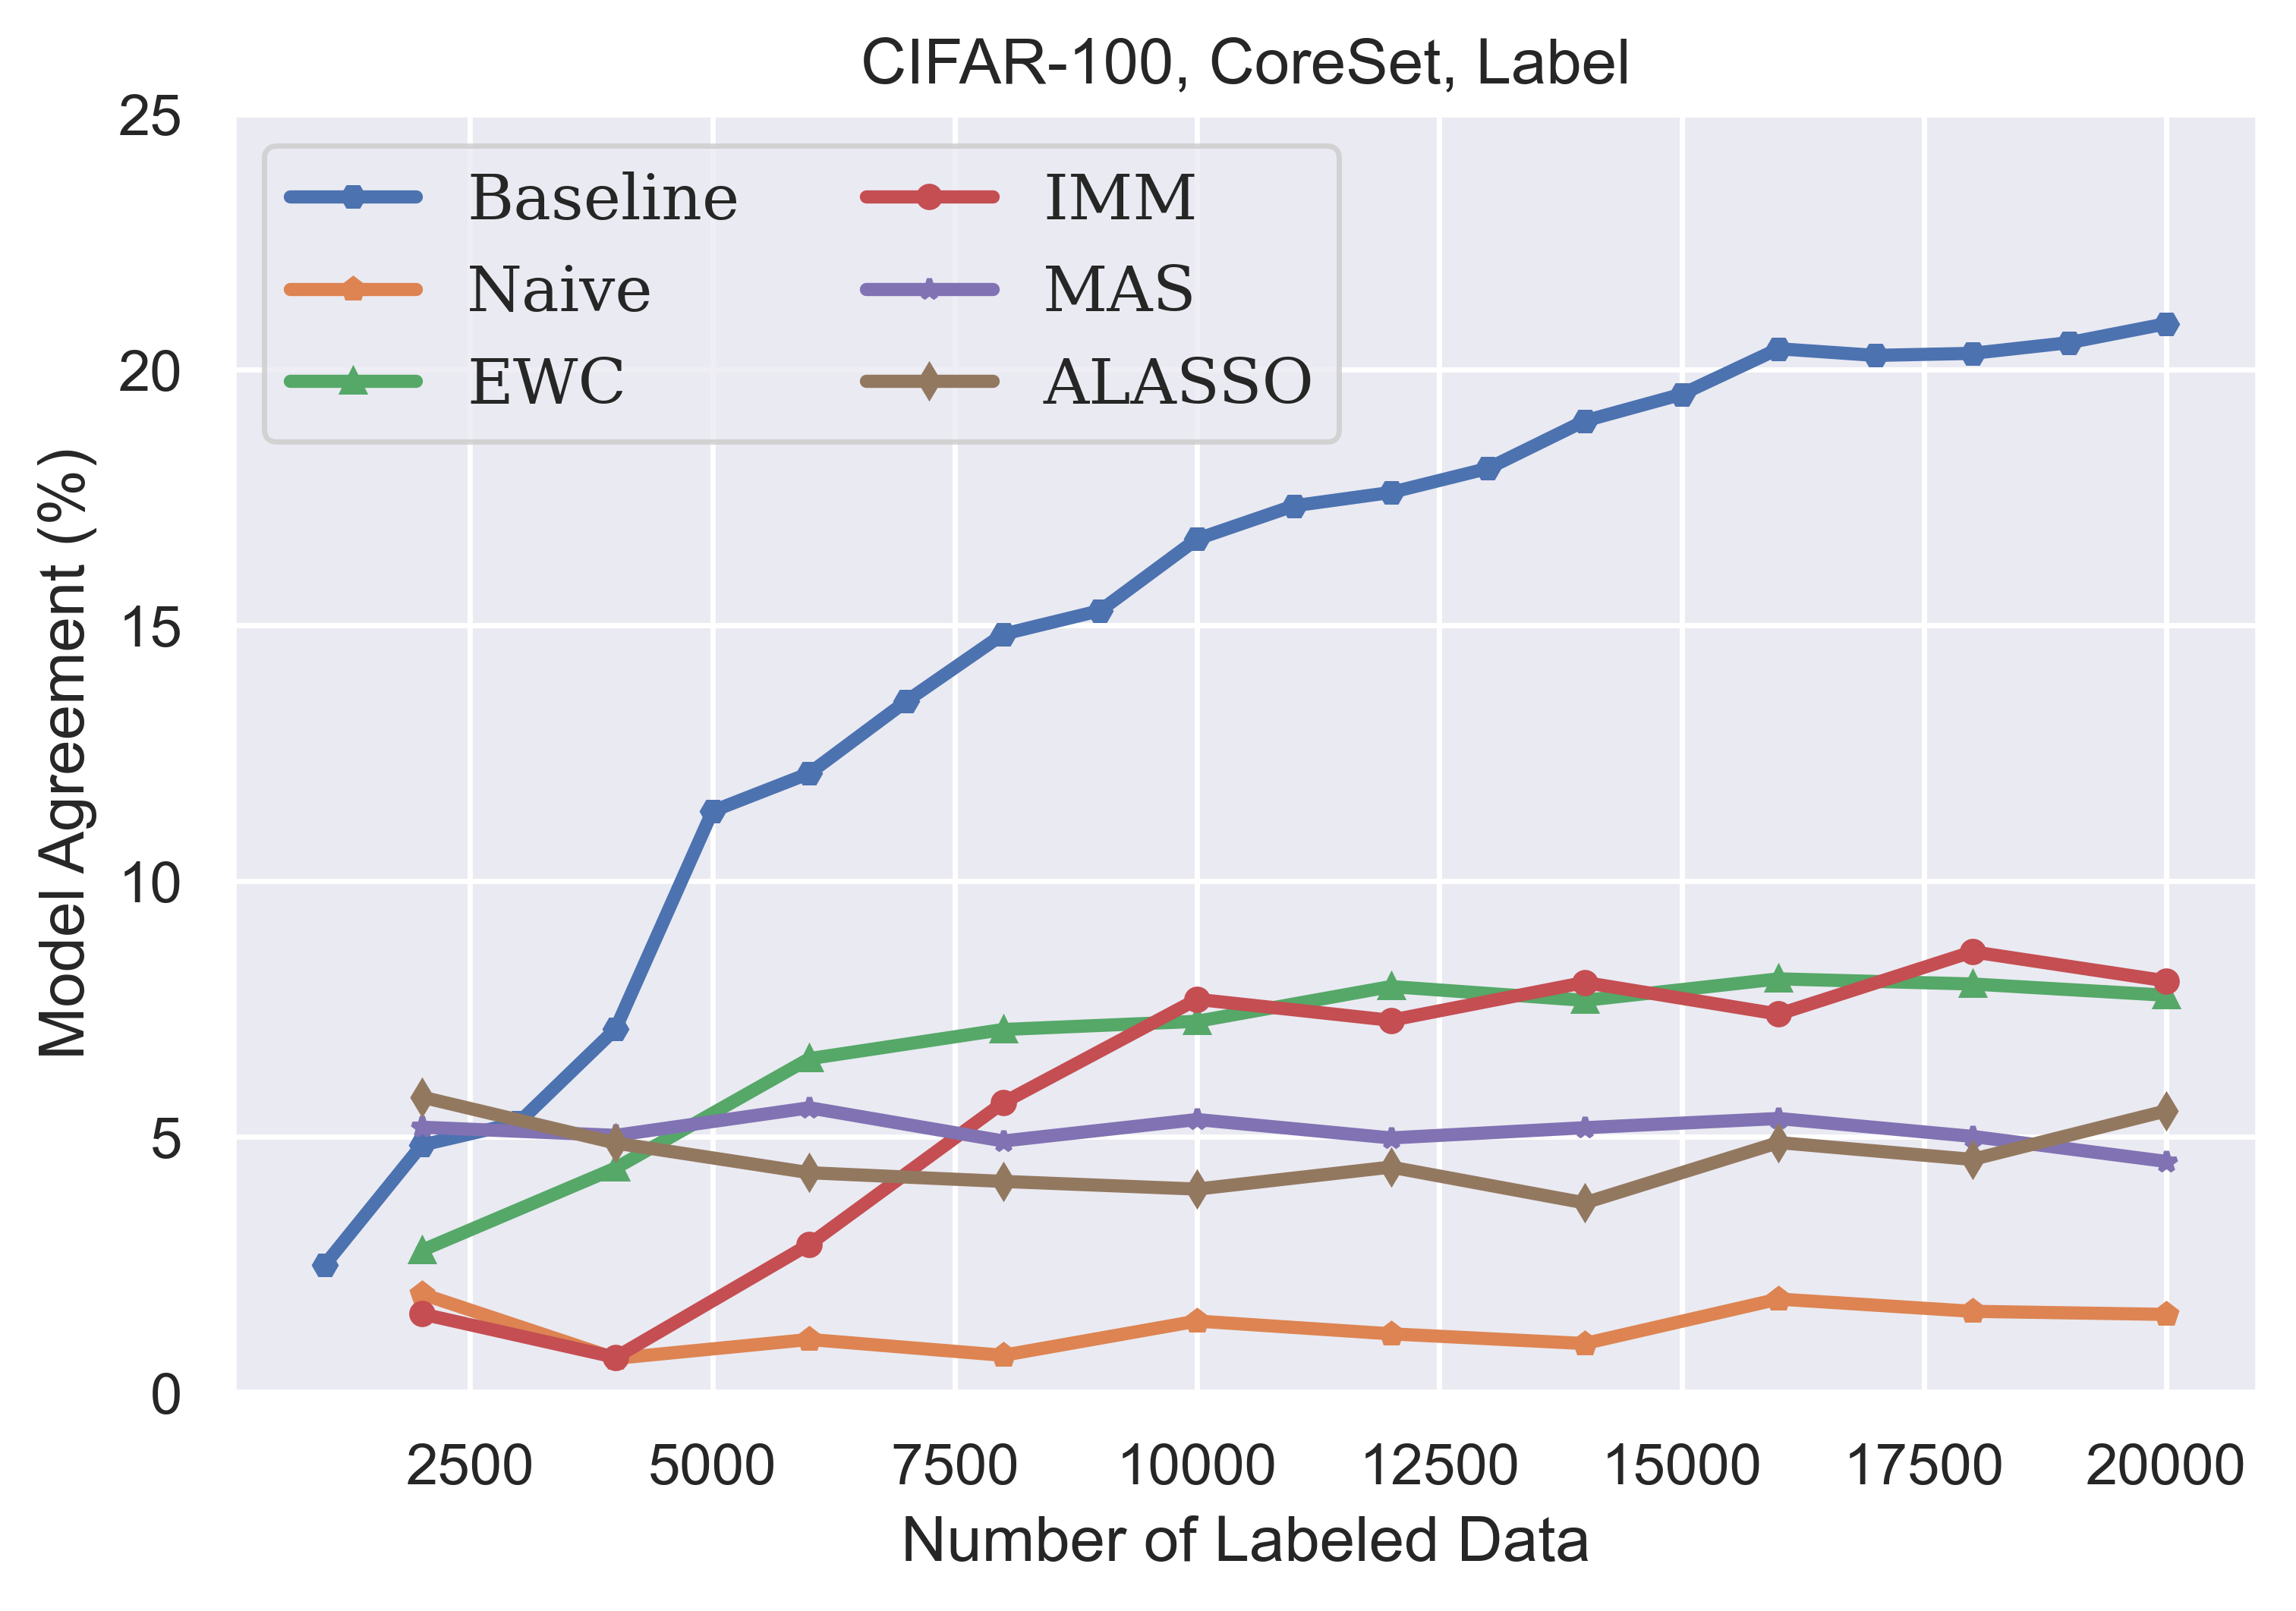
\includegraphics[width=0.5\linewidth]{images/results_CALMS/cifar100_label_coreset.png}
    \caption{Agreement Comparison for Model Stealing on CIFAR-100 using the predicted class label and the Active Learning strategy CoreSet}
    \label{fig:CALMSCIFAR100LabelCoreSet}
\end{figure}


\begin{figure}[!htb]
    \centering
    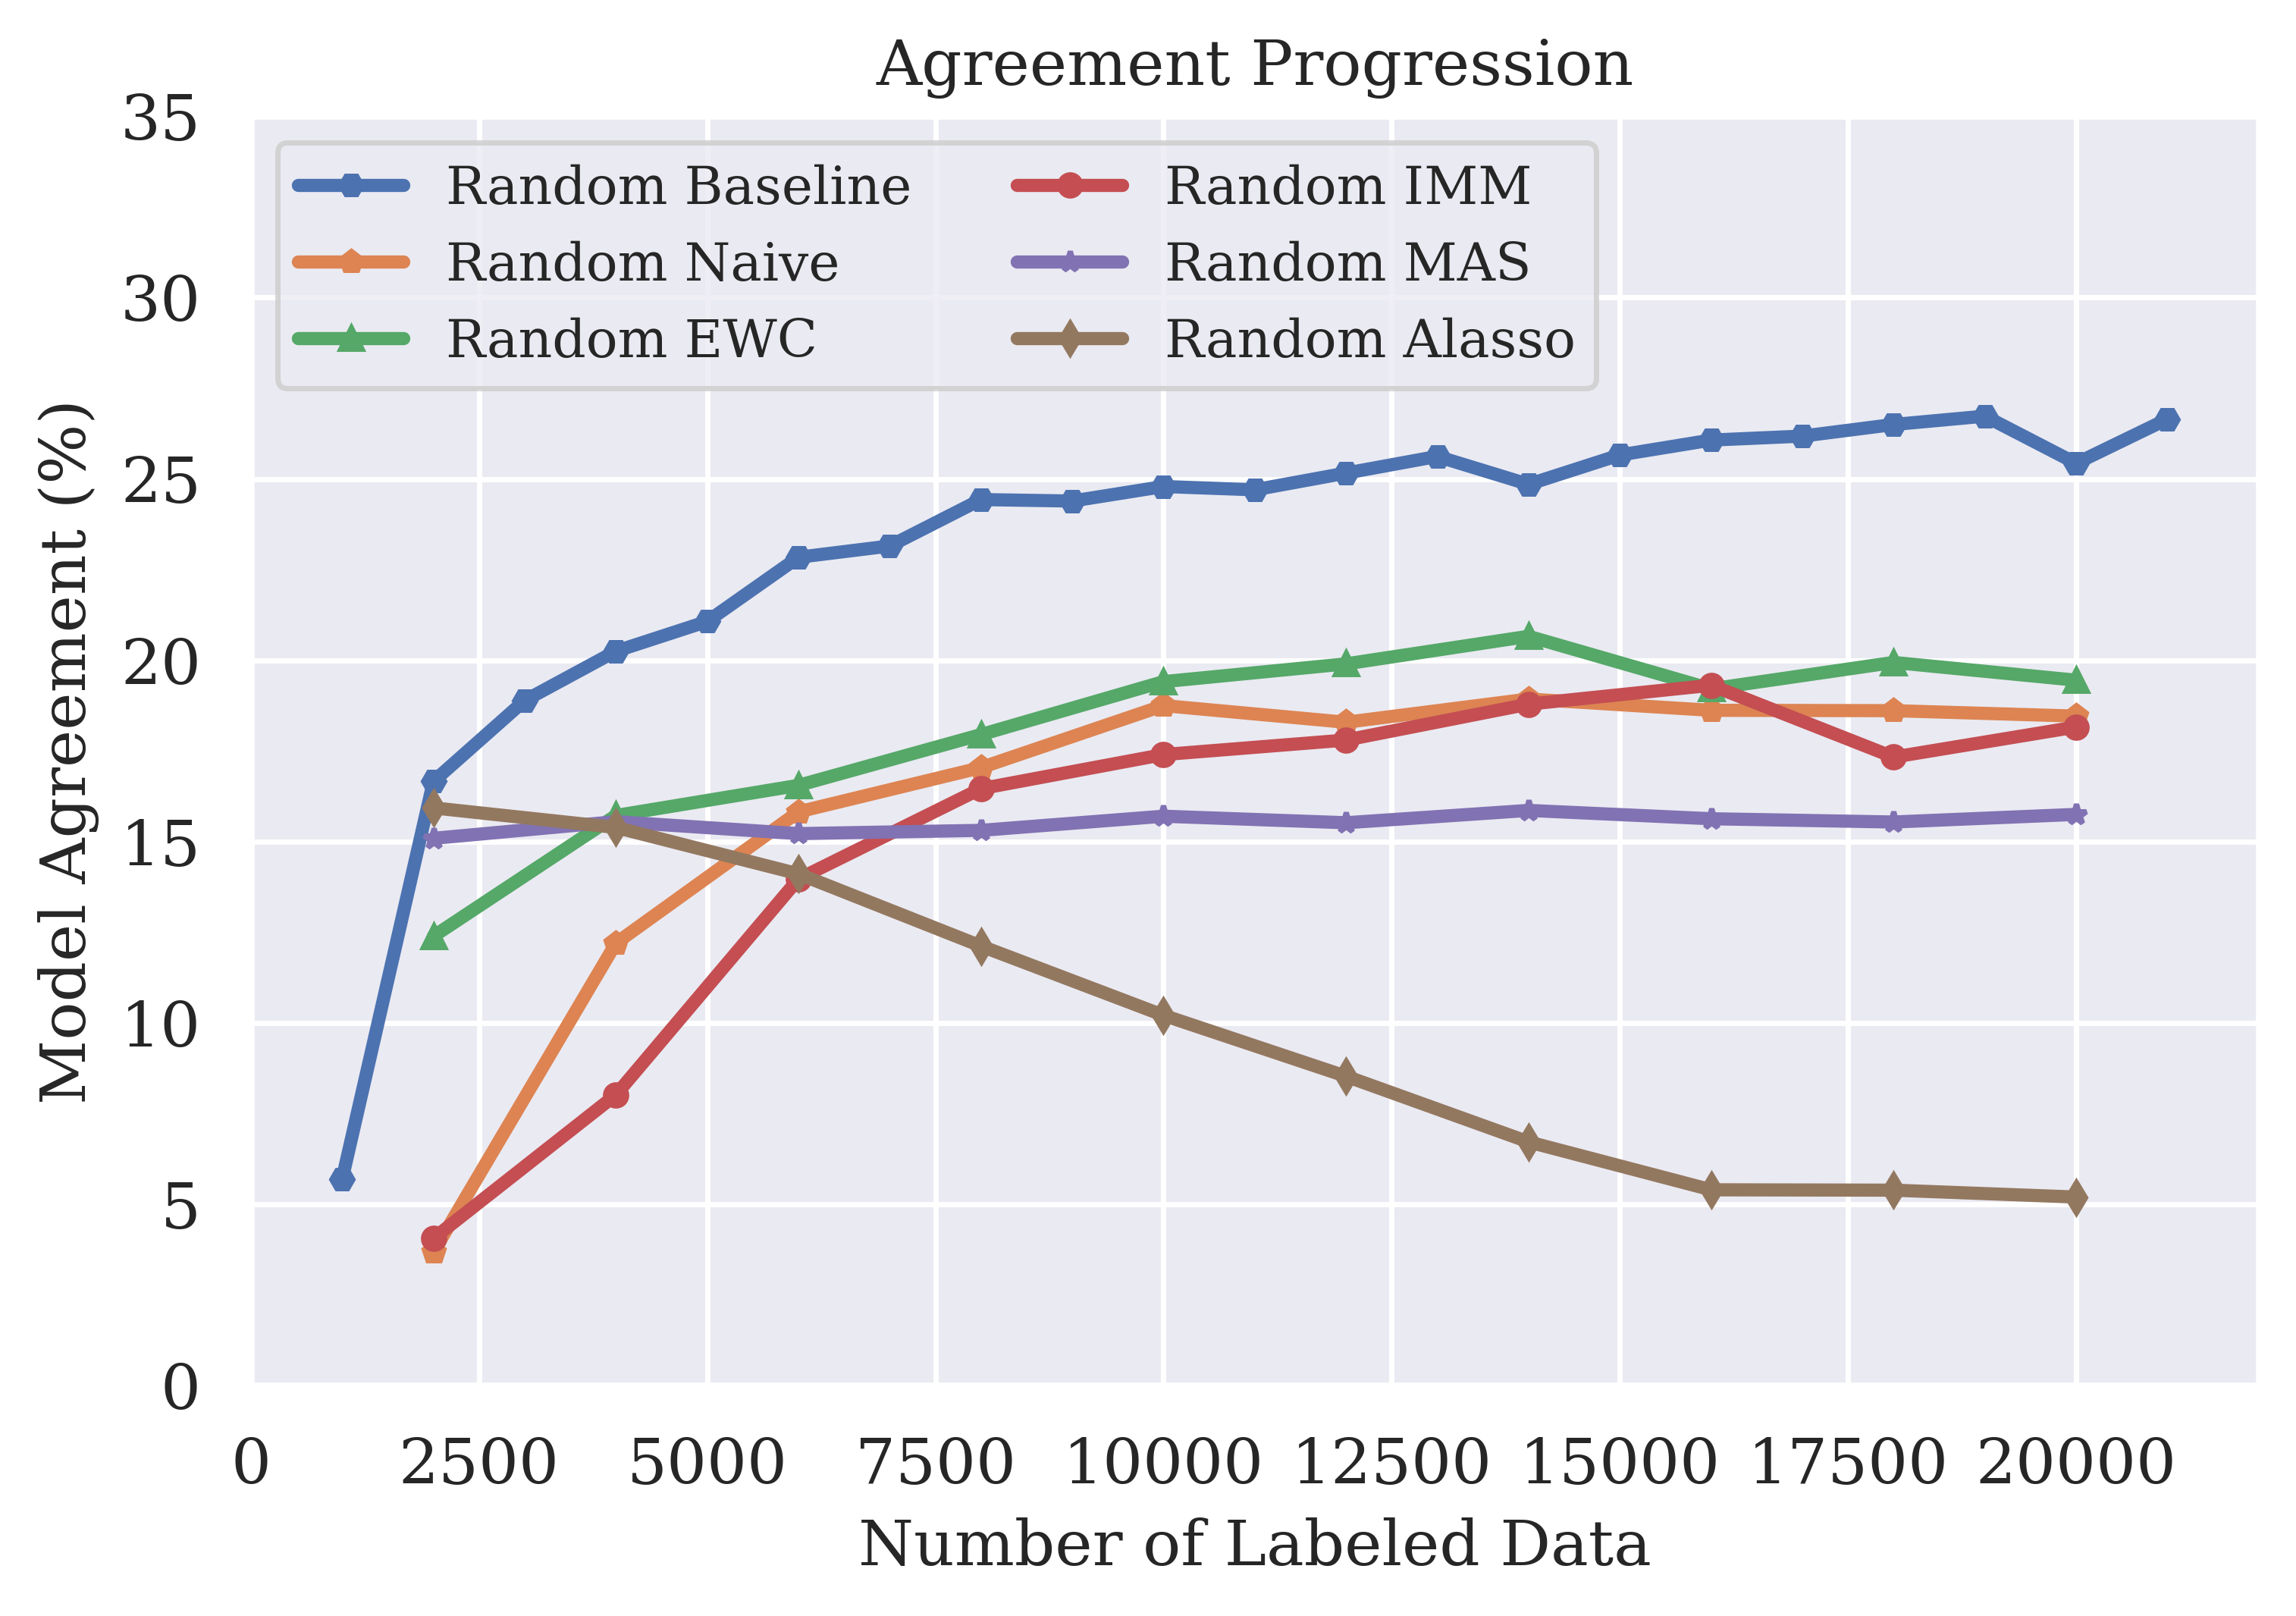
\includegraphics[width=0.5\linewidth]{images/results_CALMS/cifar100_softmax_random.png}
    \caption{Agreement Comparison for Model Stealing on CIFAR-100 using the softmax output and the Active Learning strategy Random}
    \label{fig:CALMSCIFAR100SoftmaxRandom}
\end{figure}

\begin{figure}[!htb]
    \centering
    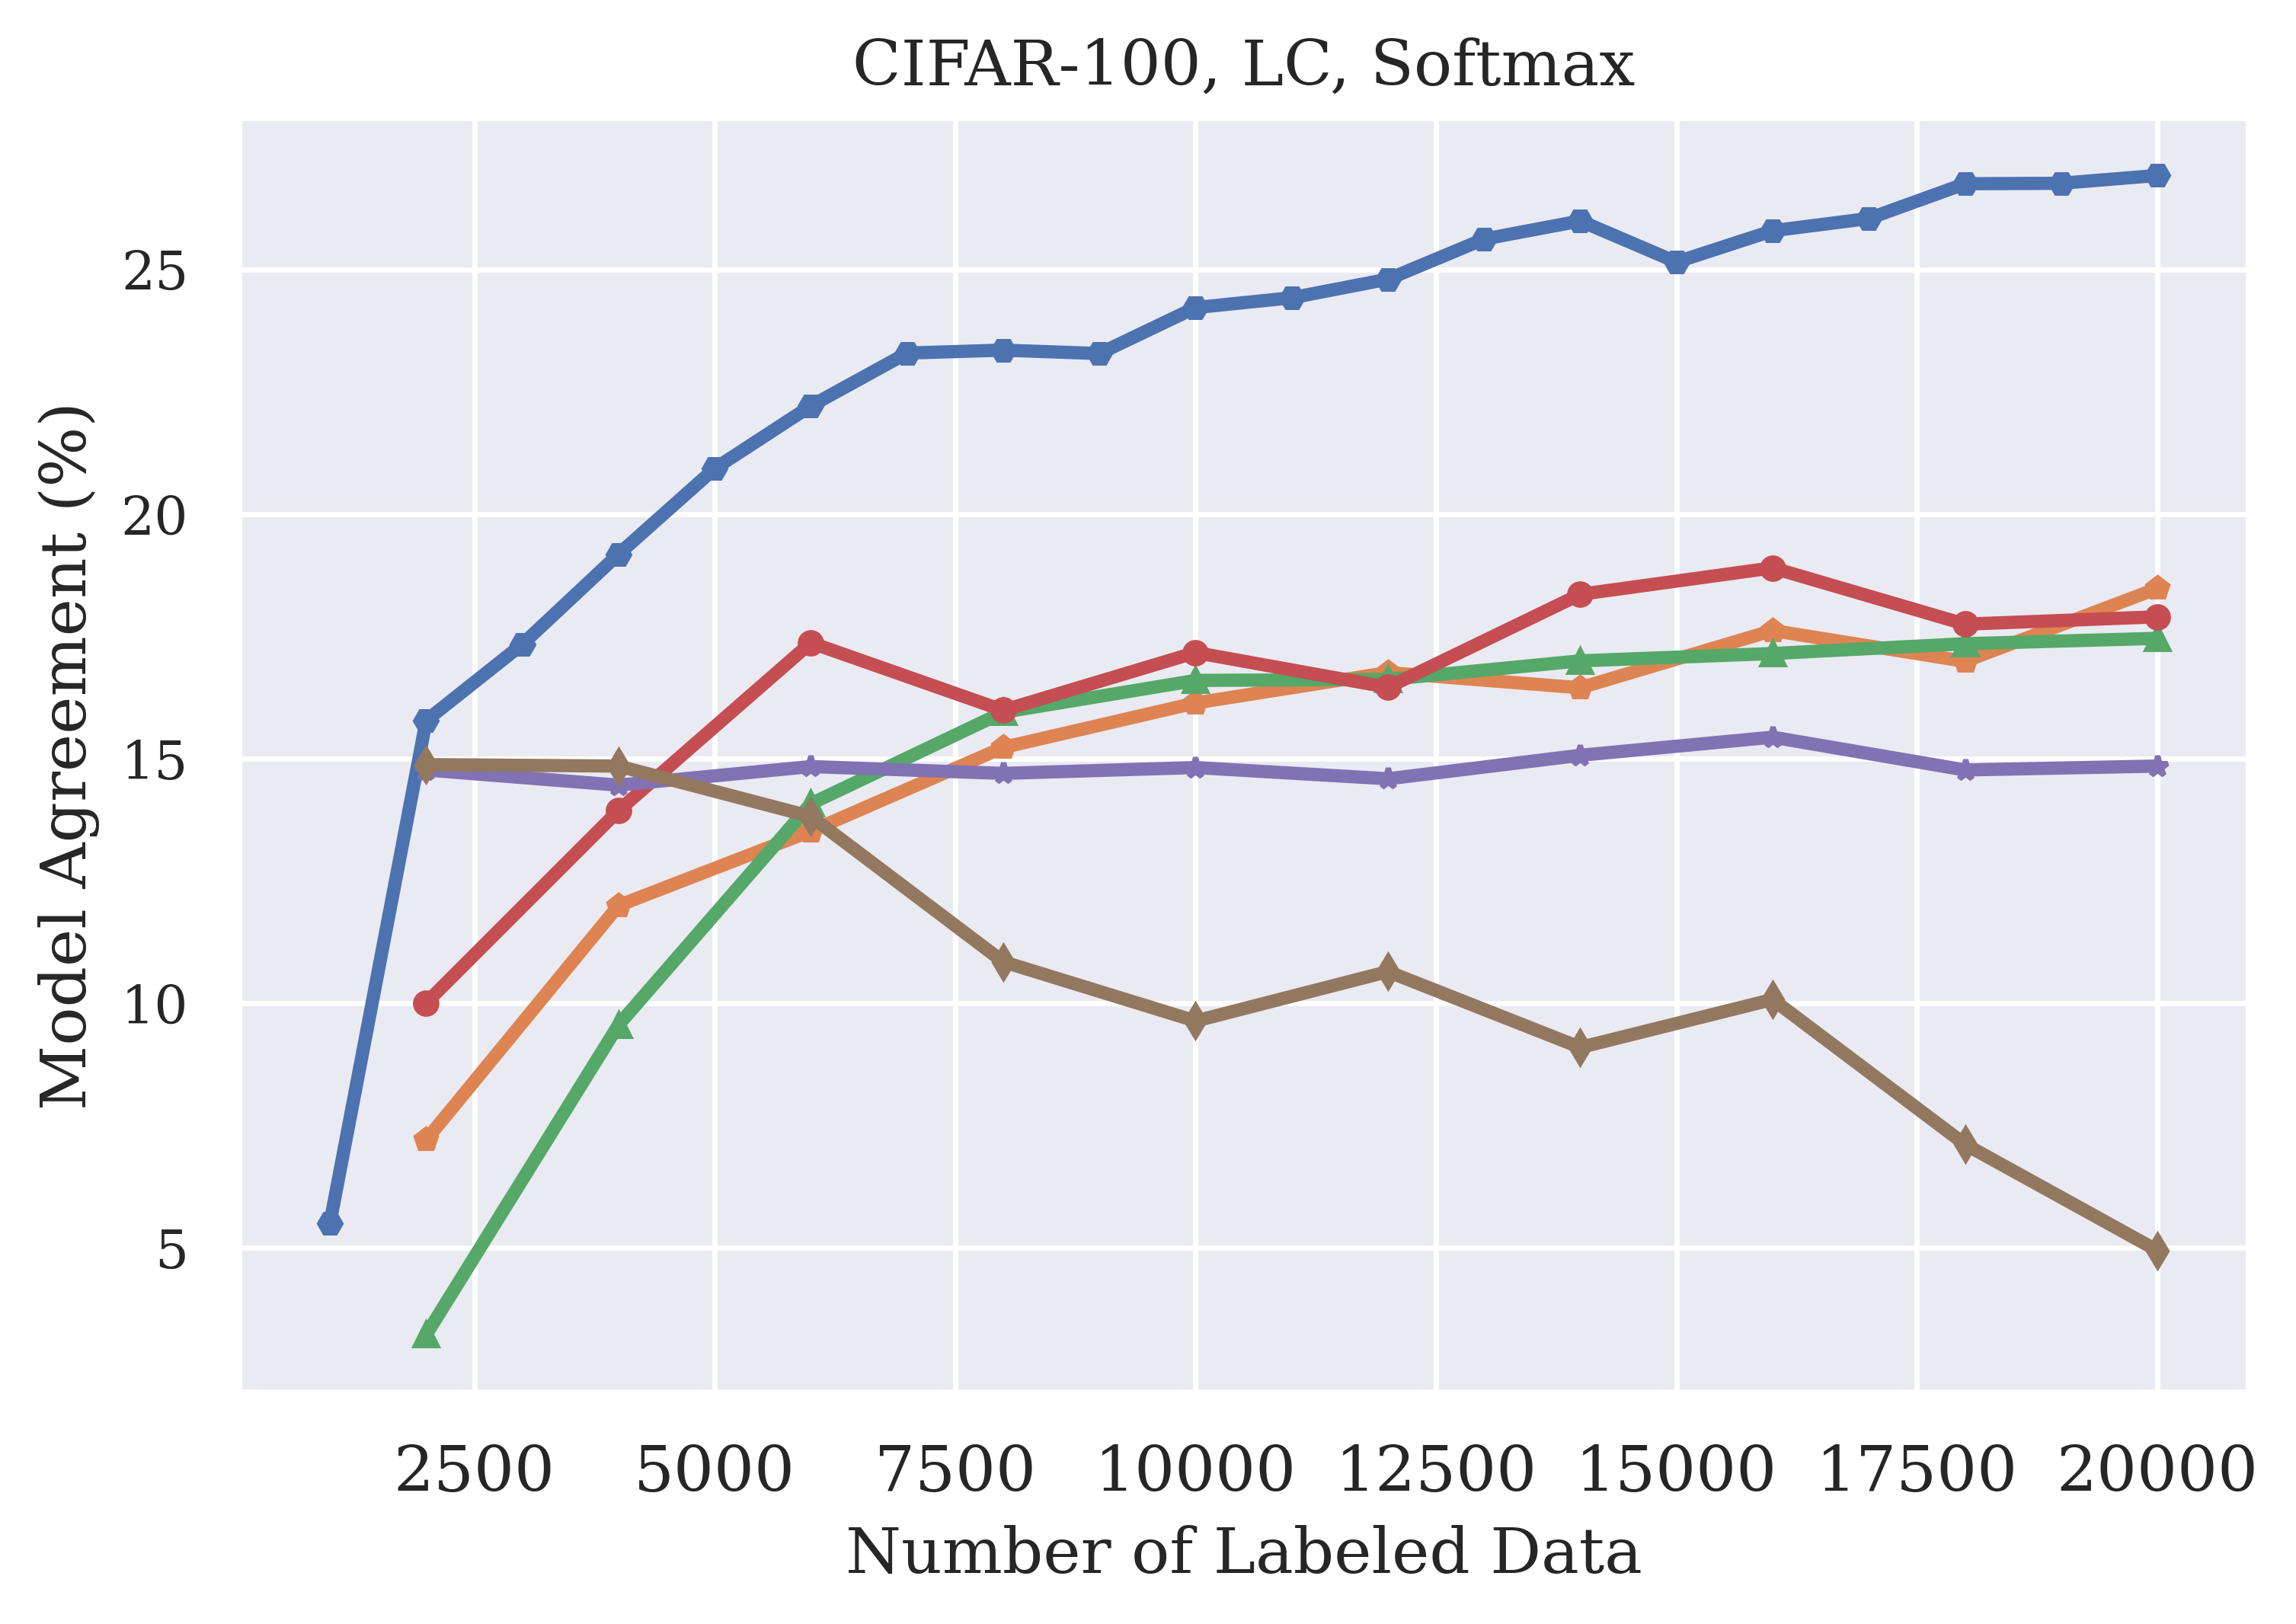
\includegraphics[width=0.5\linewidth]{images/results_CALMS/cifar100_softmax_lc.png}
    \caption{Agreement Comparison for Model Stealing on CIFAR-100 using the softmax output and the Active Learning strategy \gls{lc}}
    \label{fig:CALMSCIFAR100SoftmaxLC}
\end{figure}

\begin{figure}[!htb]
    \centering
    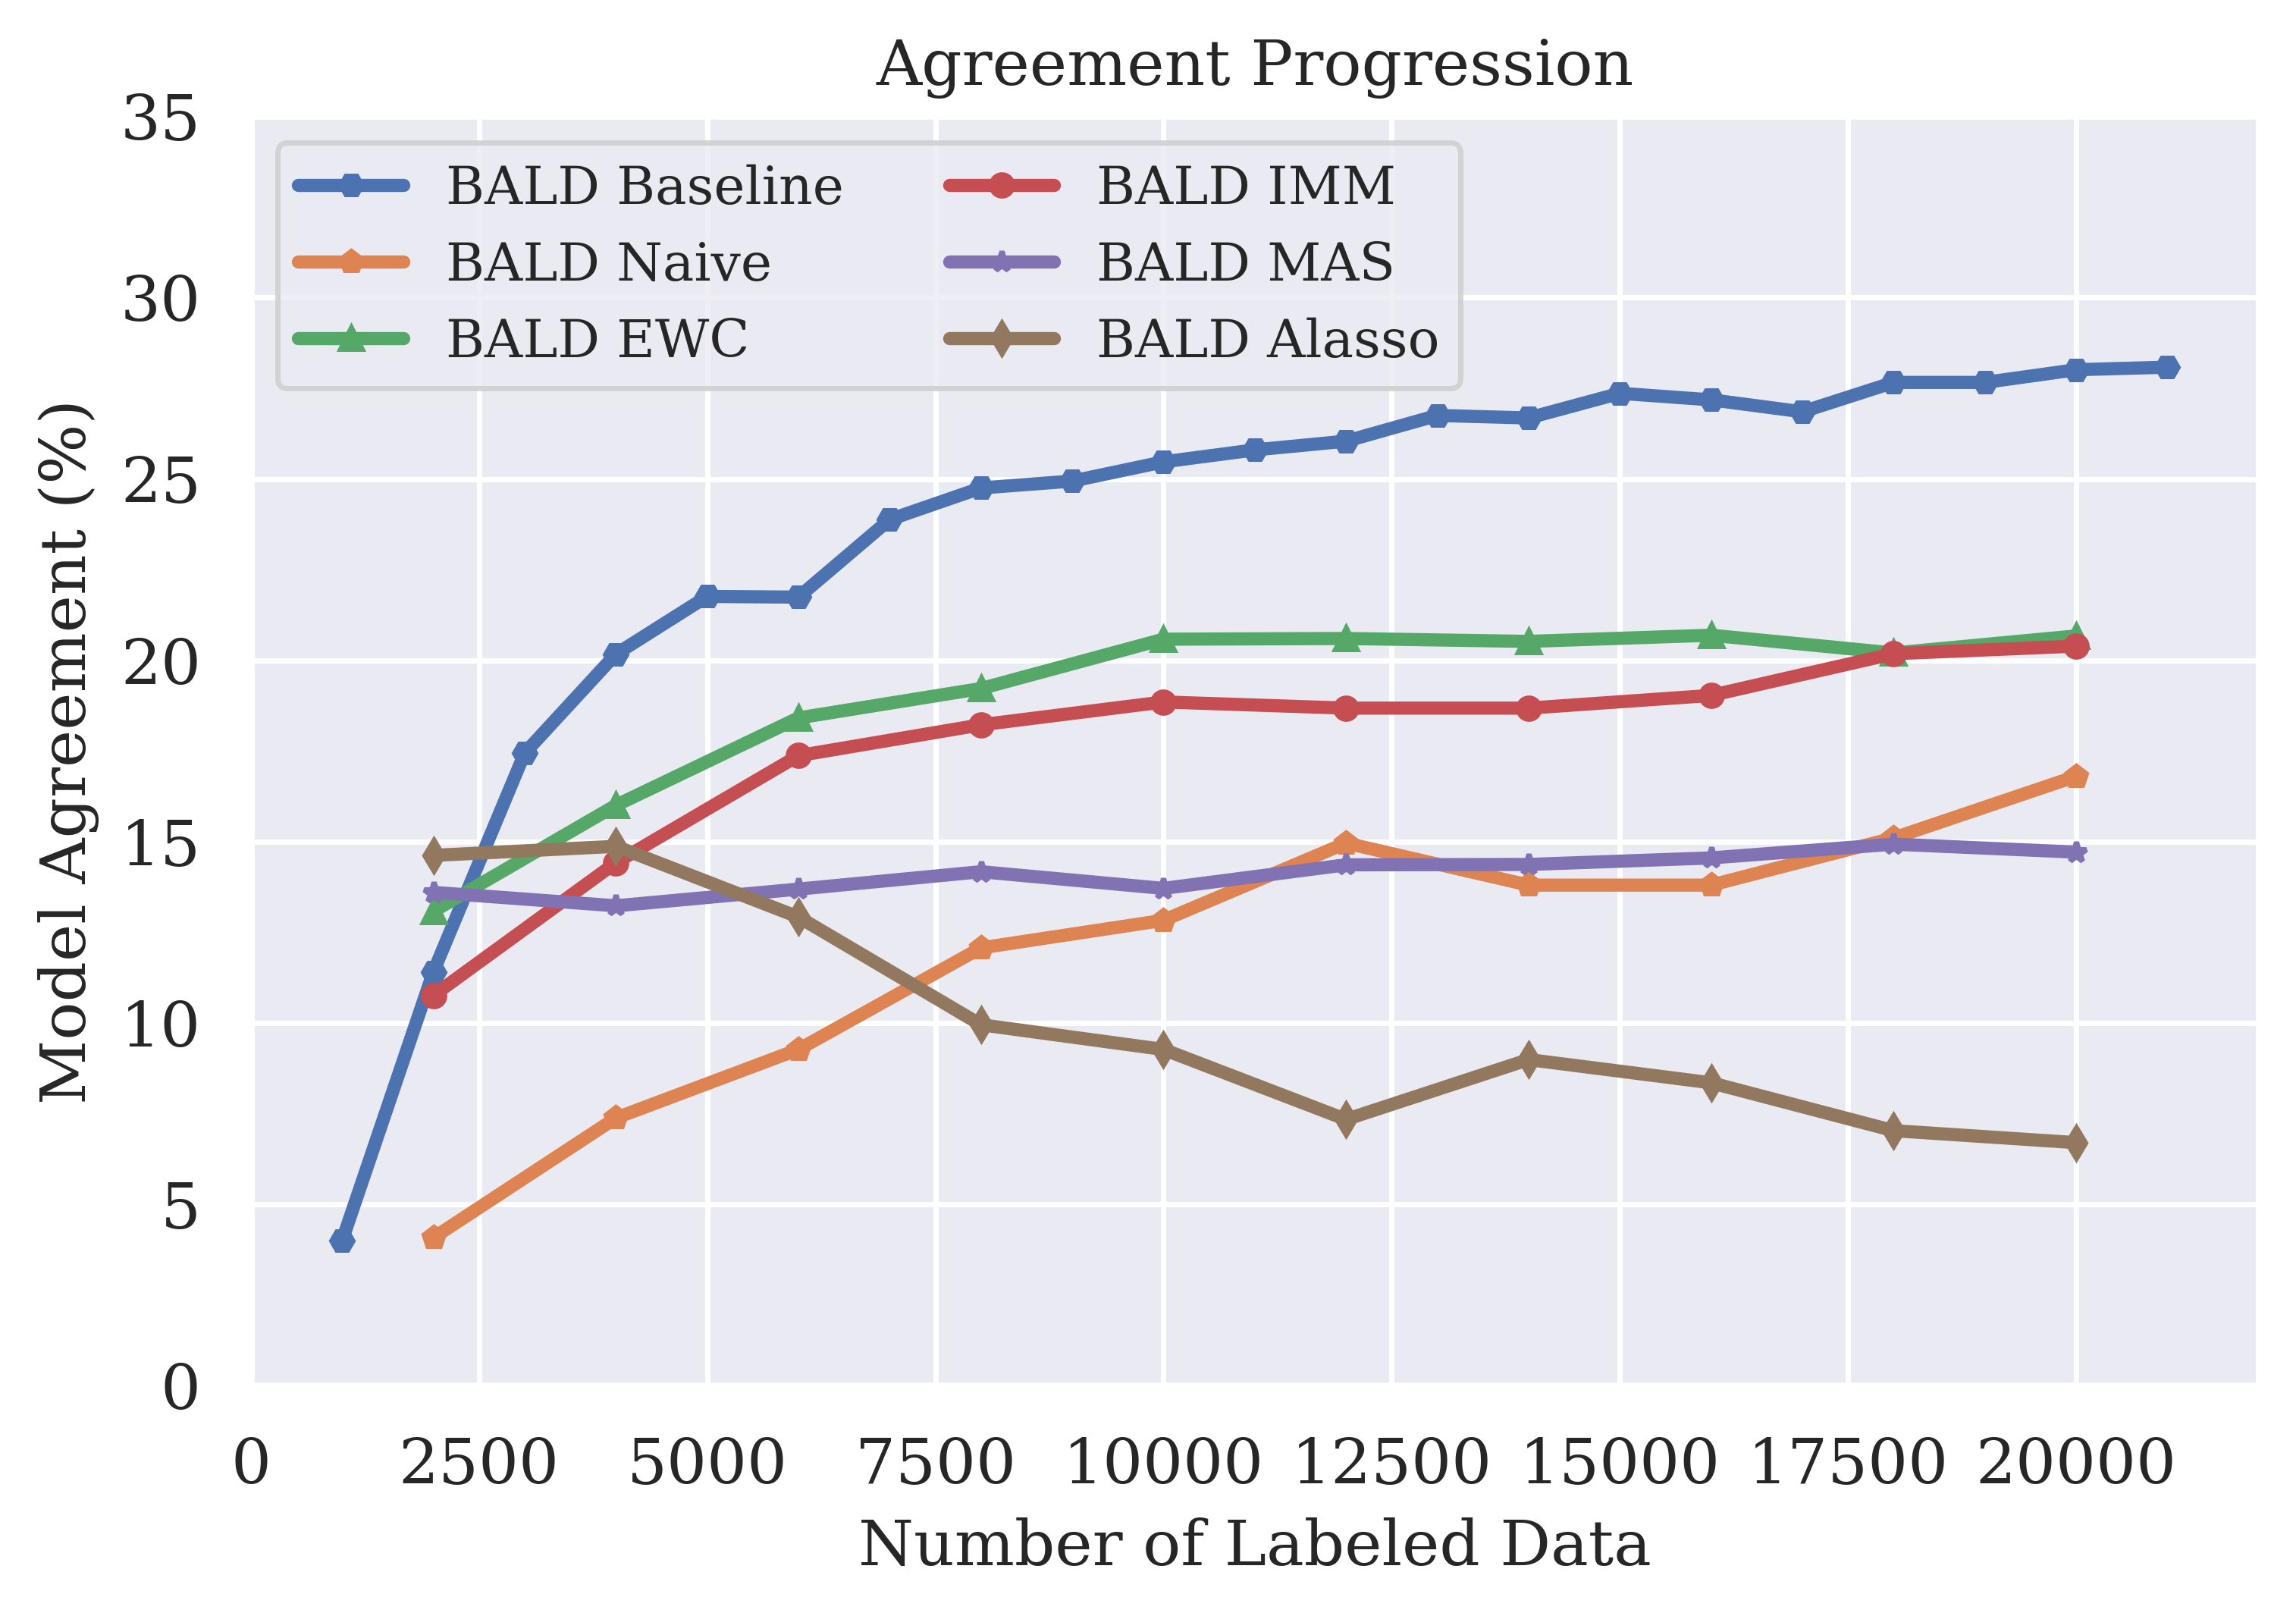
\includegraphics[width=0.5\linewidth]{images/results_CALMS/cifar100_softmax_bald.png}
    \caption{Agreement Comparison for Model Stealing on CIFAR-100 using the softmax output and the Active Learning strategy \gls{bald}}
    \label{fig:CALMSCIFAR100SoftmaxBALD}
\end{figure}

\begin{figure}[!htb]
    \centering
    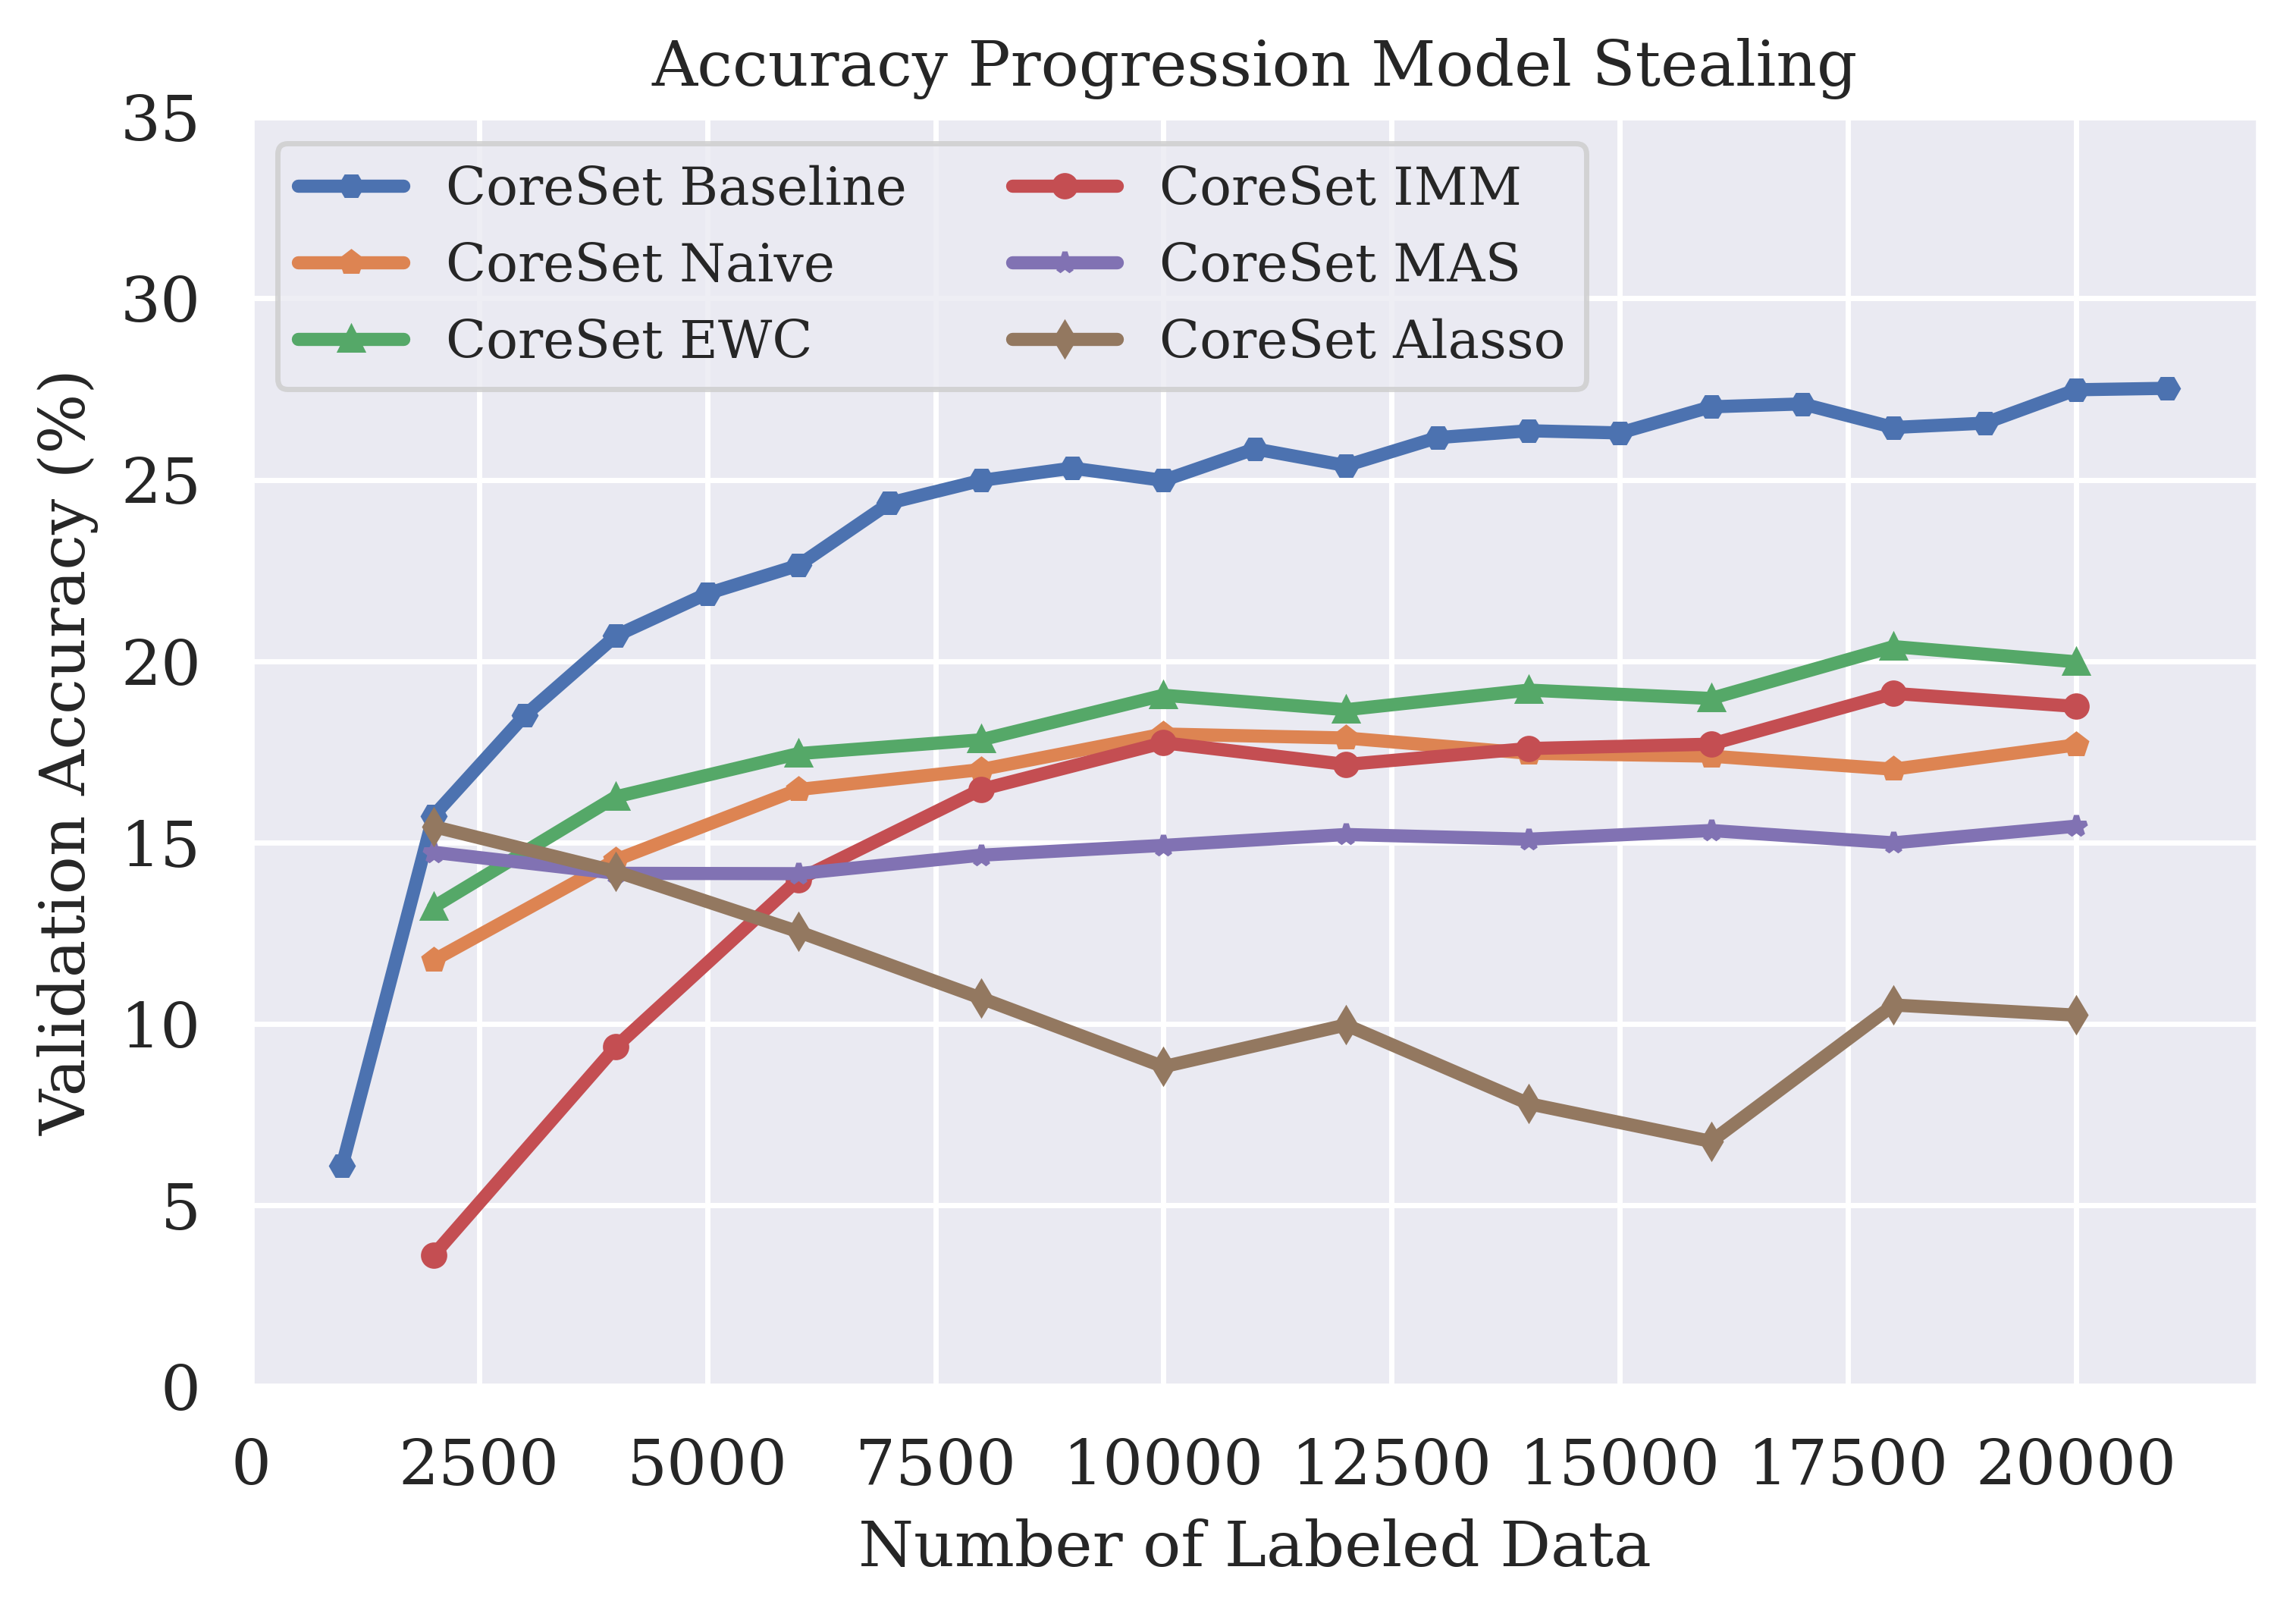
\includegraphics[width=0.5\linewidth]{images/results_CALMS/cifar100_softmax_coreset.png}
    \caption{Agreement Comparison for Model Stealing on CIFAR-100 using the softmax output and the Active Learning strategy CoreSet}
    \label{fig:CALMSCIFAR100SoftmaxCoreSet}
\end{figure}

\subsubsection{VAAL and A-GEM}
\label{sec:Appendix:CALMS:VAALAGEM}
In the following we list the full results for the experiments using \gls{vaal} and \gls{a-gem} on the dataset MNIST, CIFAR-10 and CIFAR-100.
\begin{figure}[!htb]
    \centering
    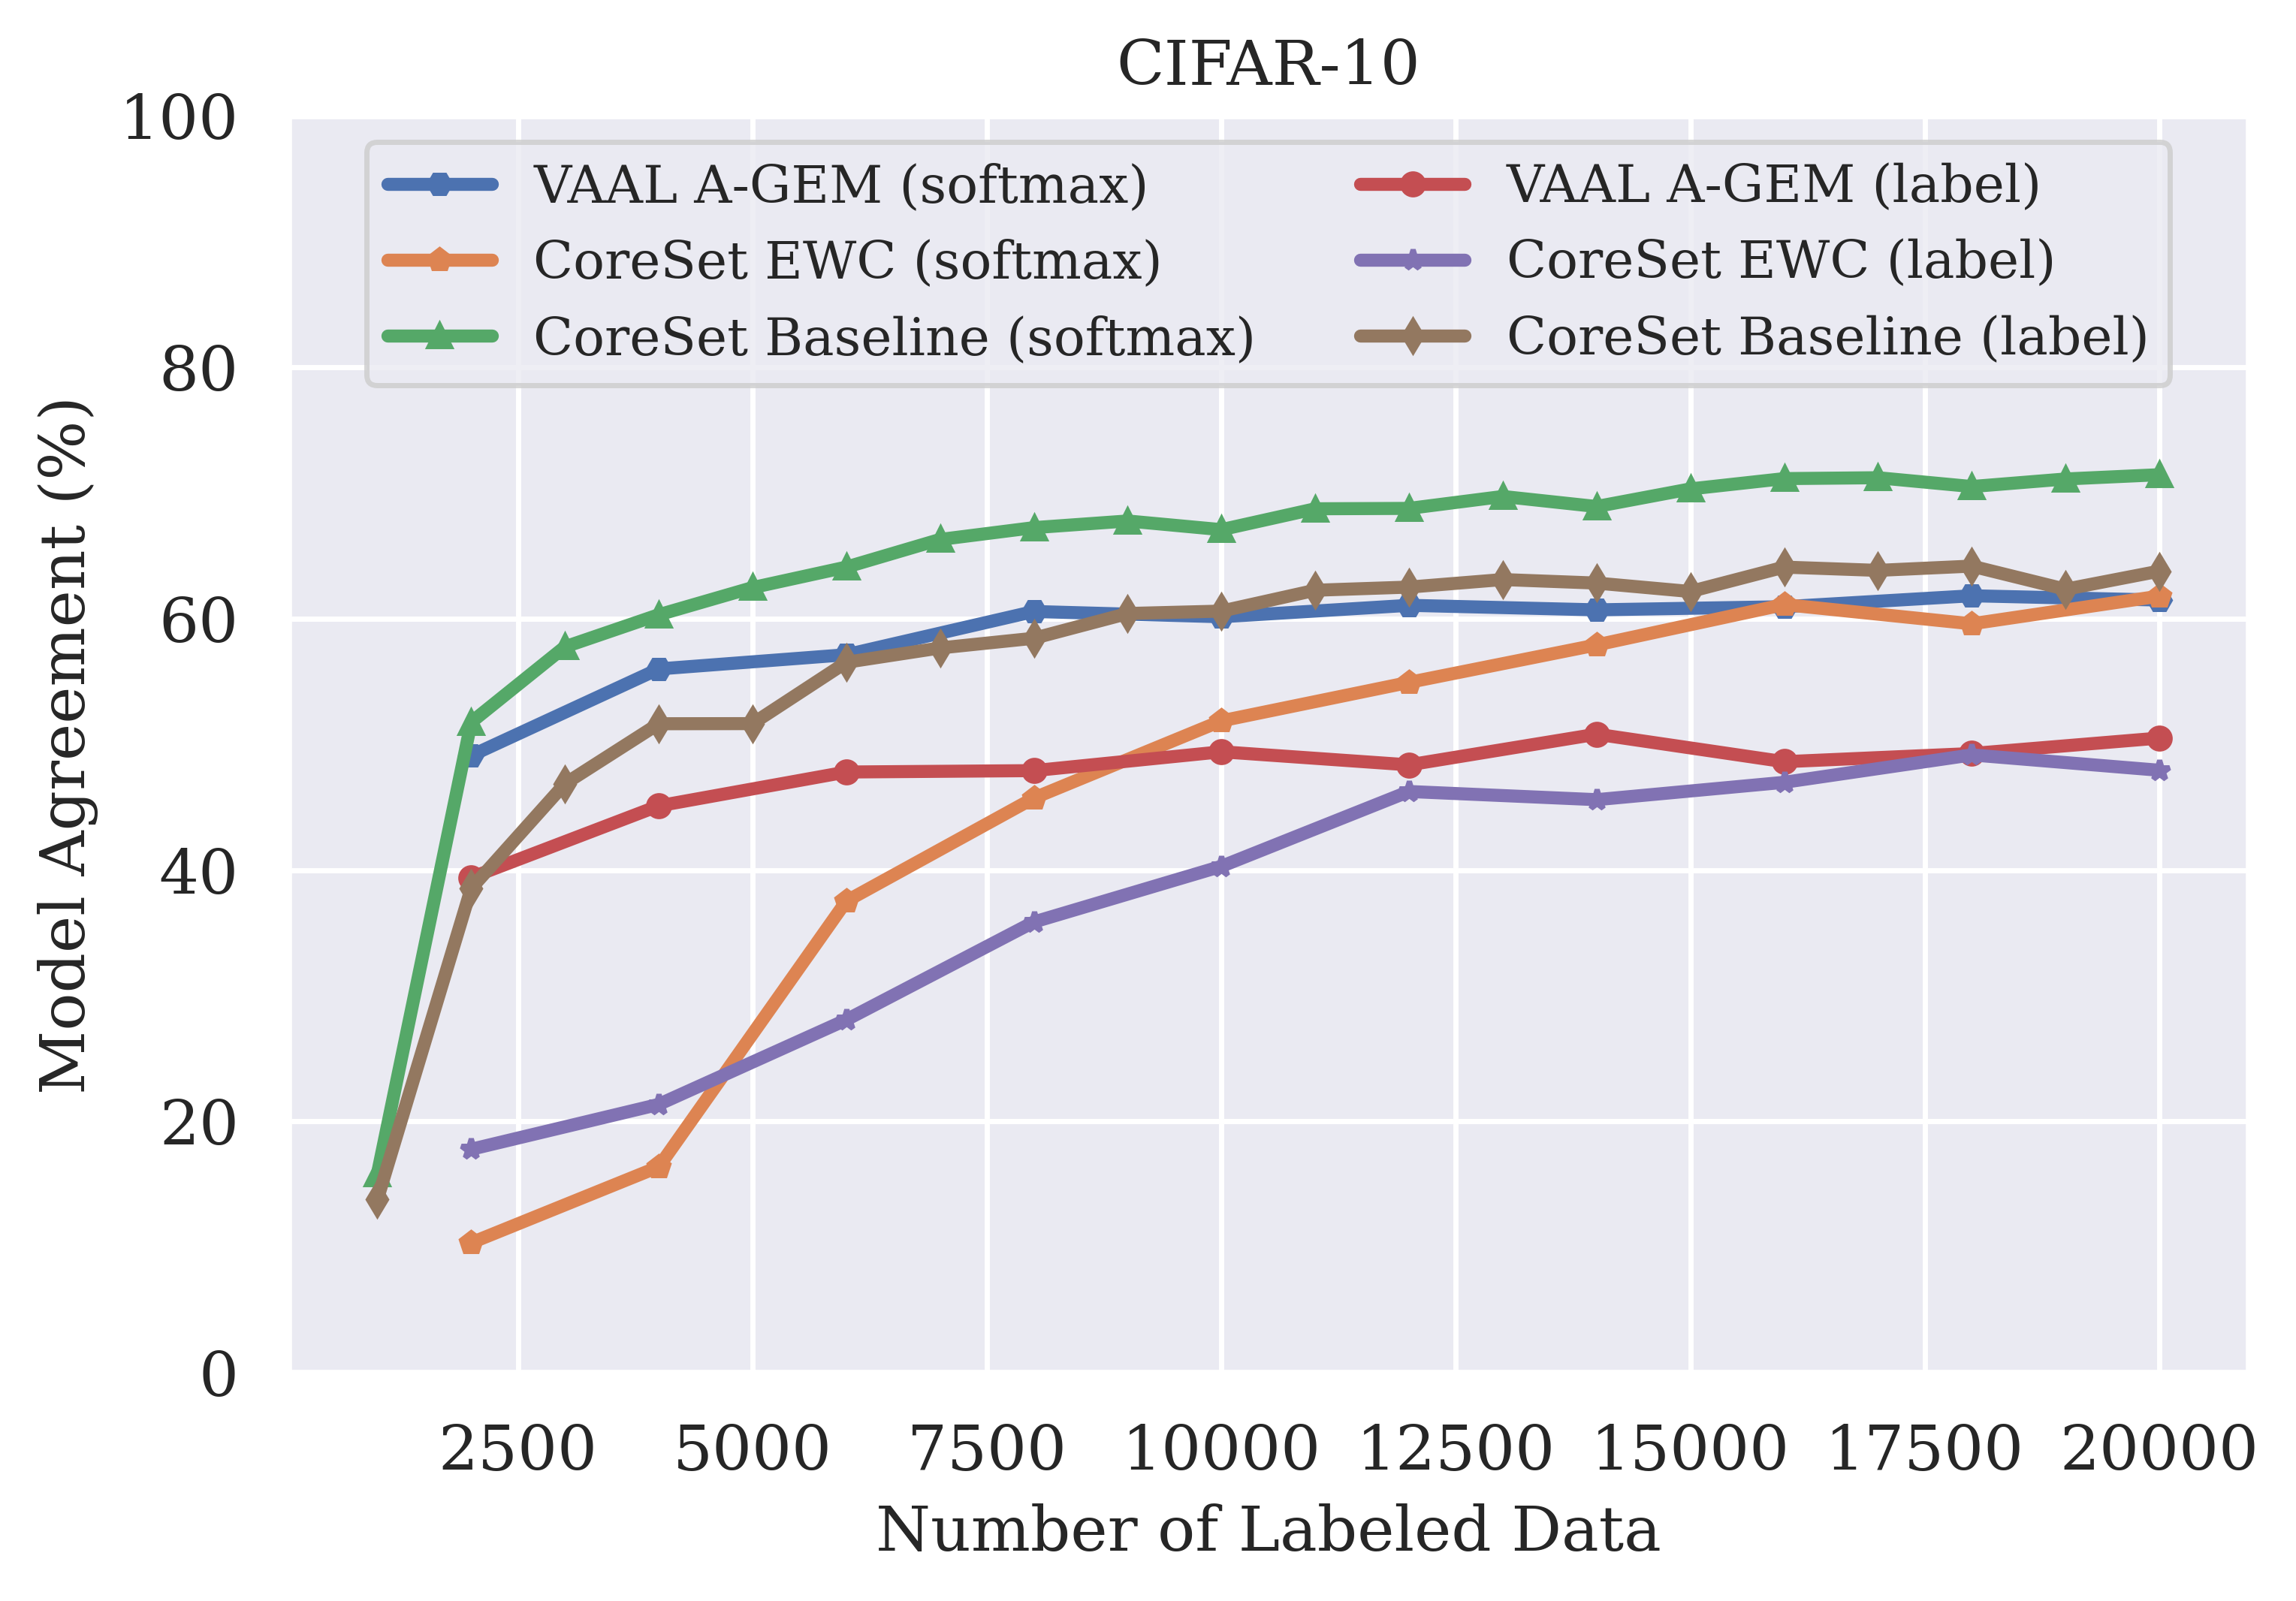
\includegraphics[width=0.5\linewidth]{images/results_CALMS/cifar_vaal_agem.png}
    \caption{Agreement Comparison for Model Stealing on CIFAR-10 using \gls{vaal} and \gls{a-gem}}
    \label{fig:CALMScifarVAAL_AGEM}
\end{figure}

\begin{figure}[!htb]
    \centering
    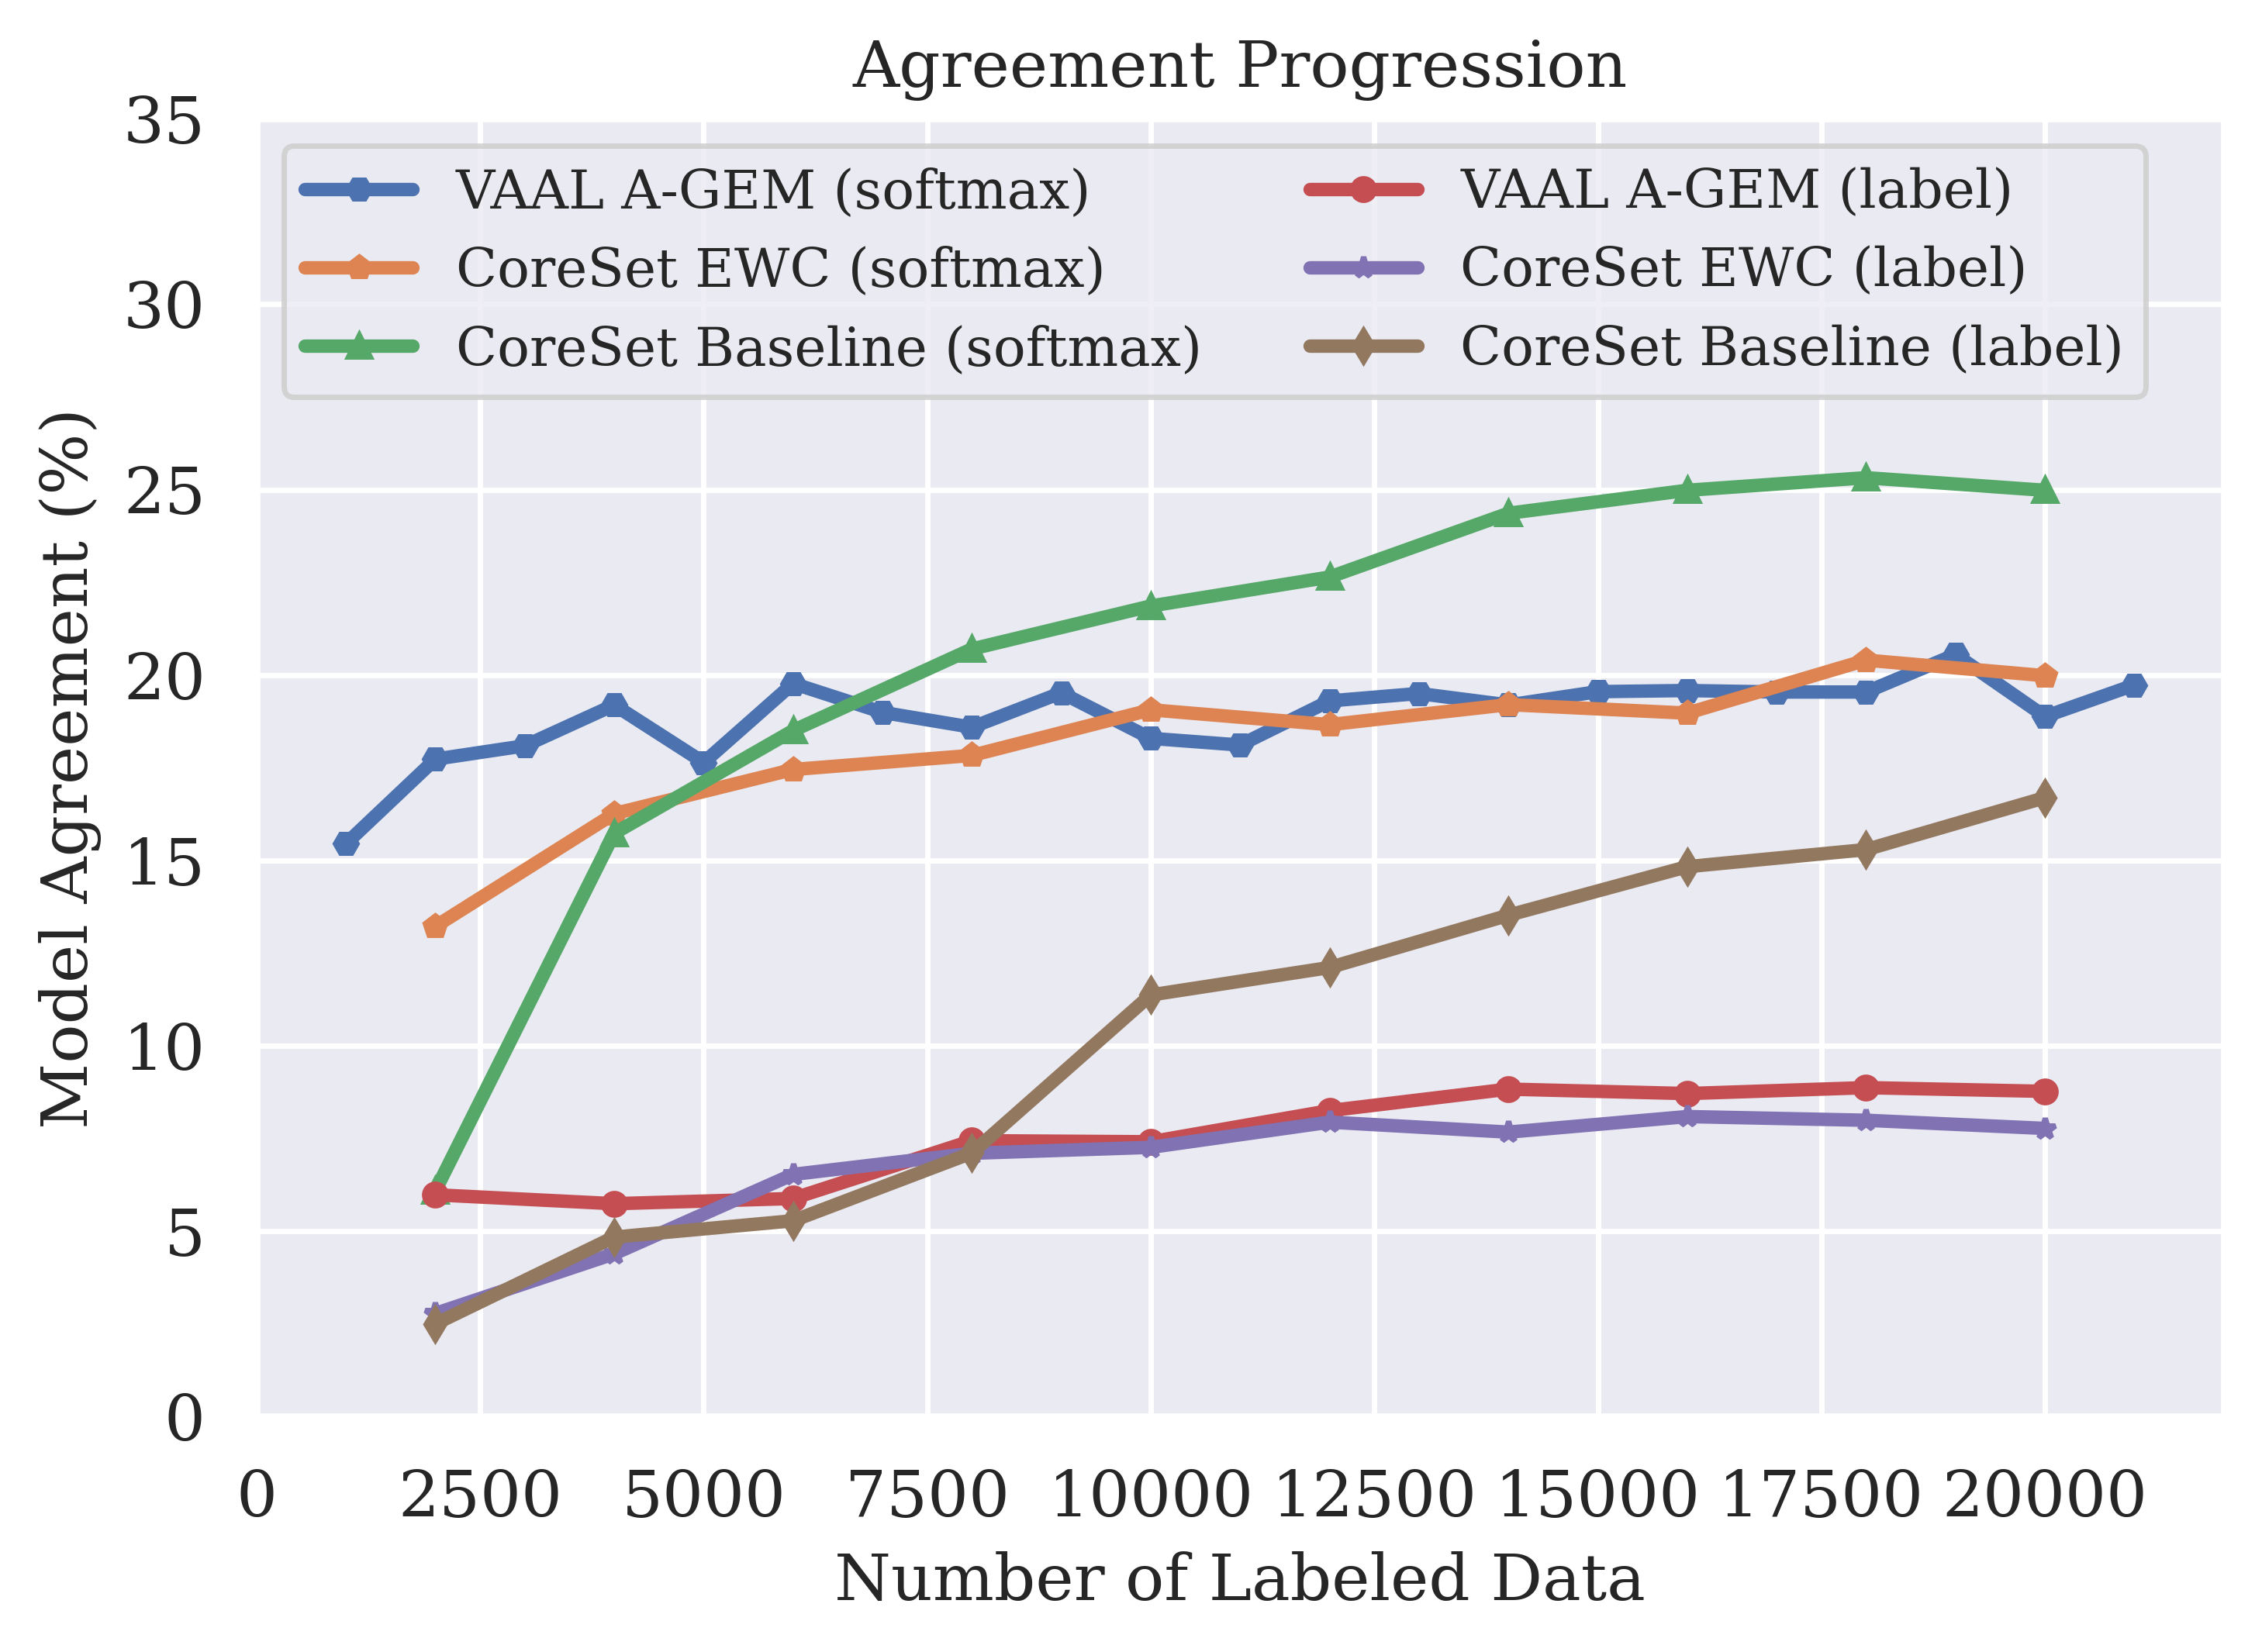
\includegraphics[width=0.5\linewidth]{images/results_CALMS/cifar100_vaal_agem.png}
    \caption{Agreement Comparison for Model Stealing on CIFAR-100 using \gls{vaal} and \gls{a-gem}}
    \label{fig:CALMScifar100VAAL_AGEM}
\end{figure}

\begin{figure}[!htb]
    \centering
    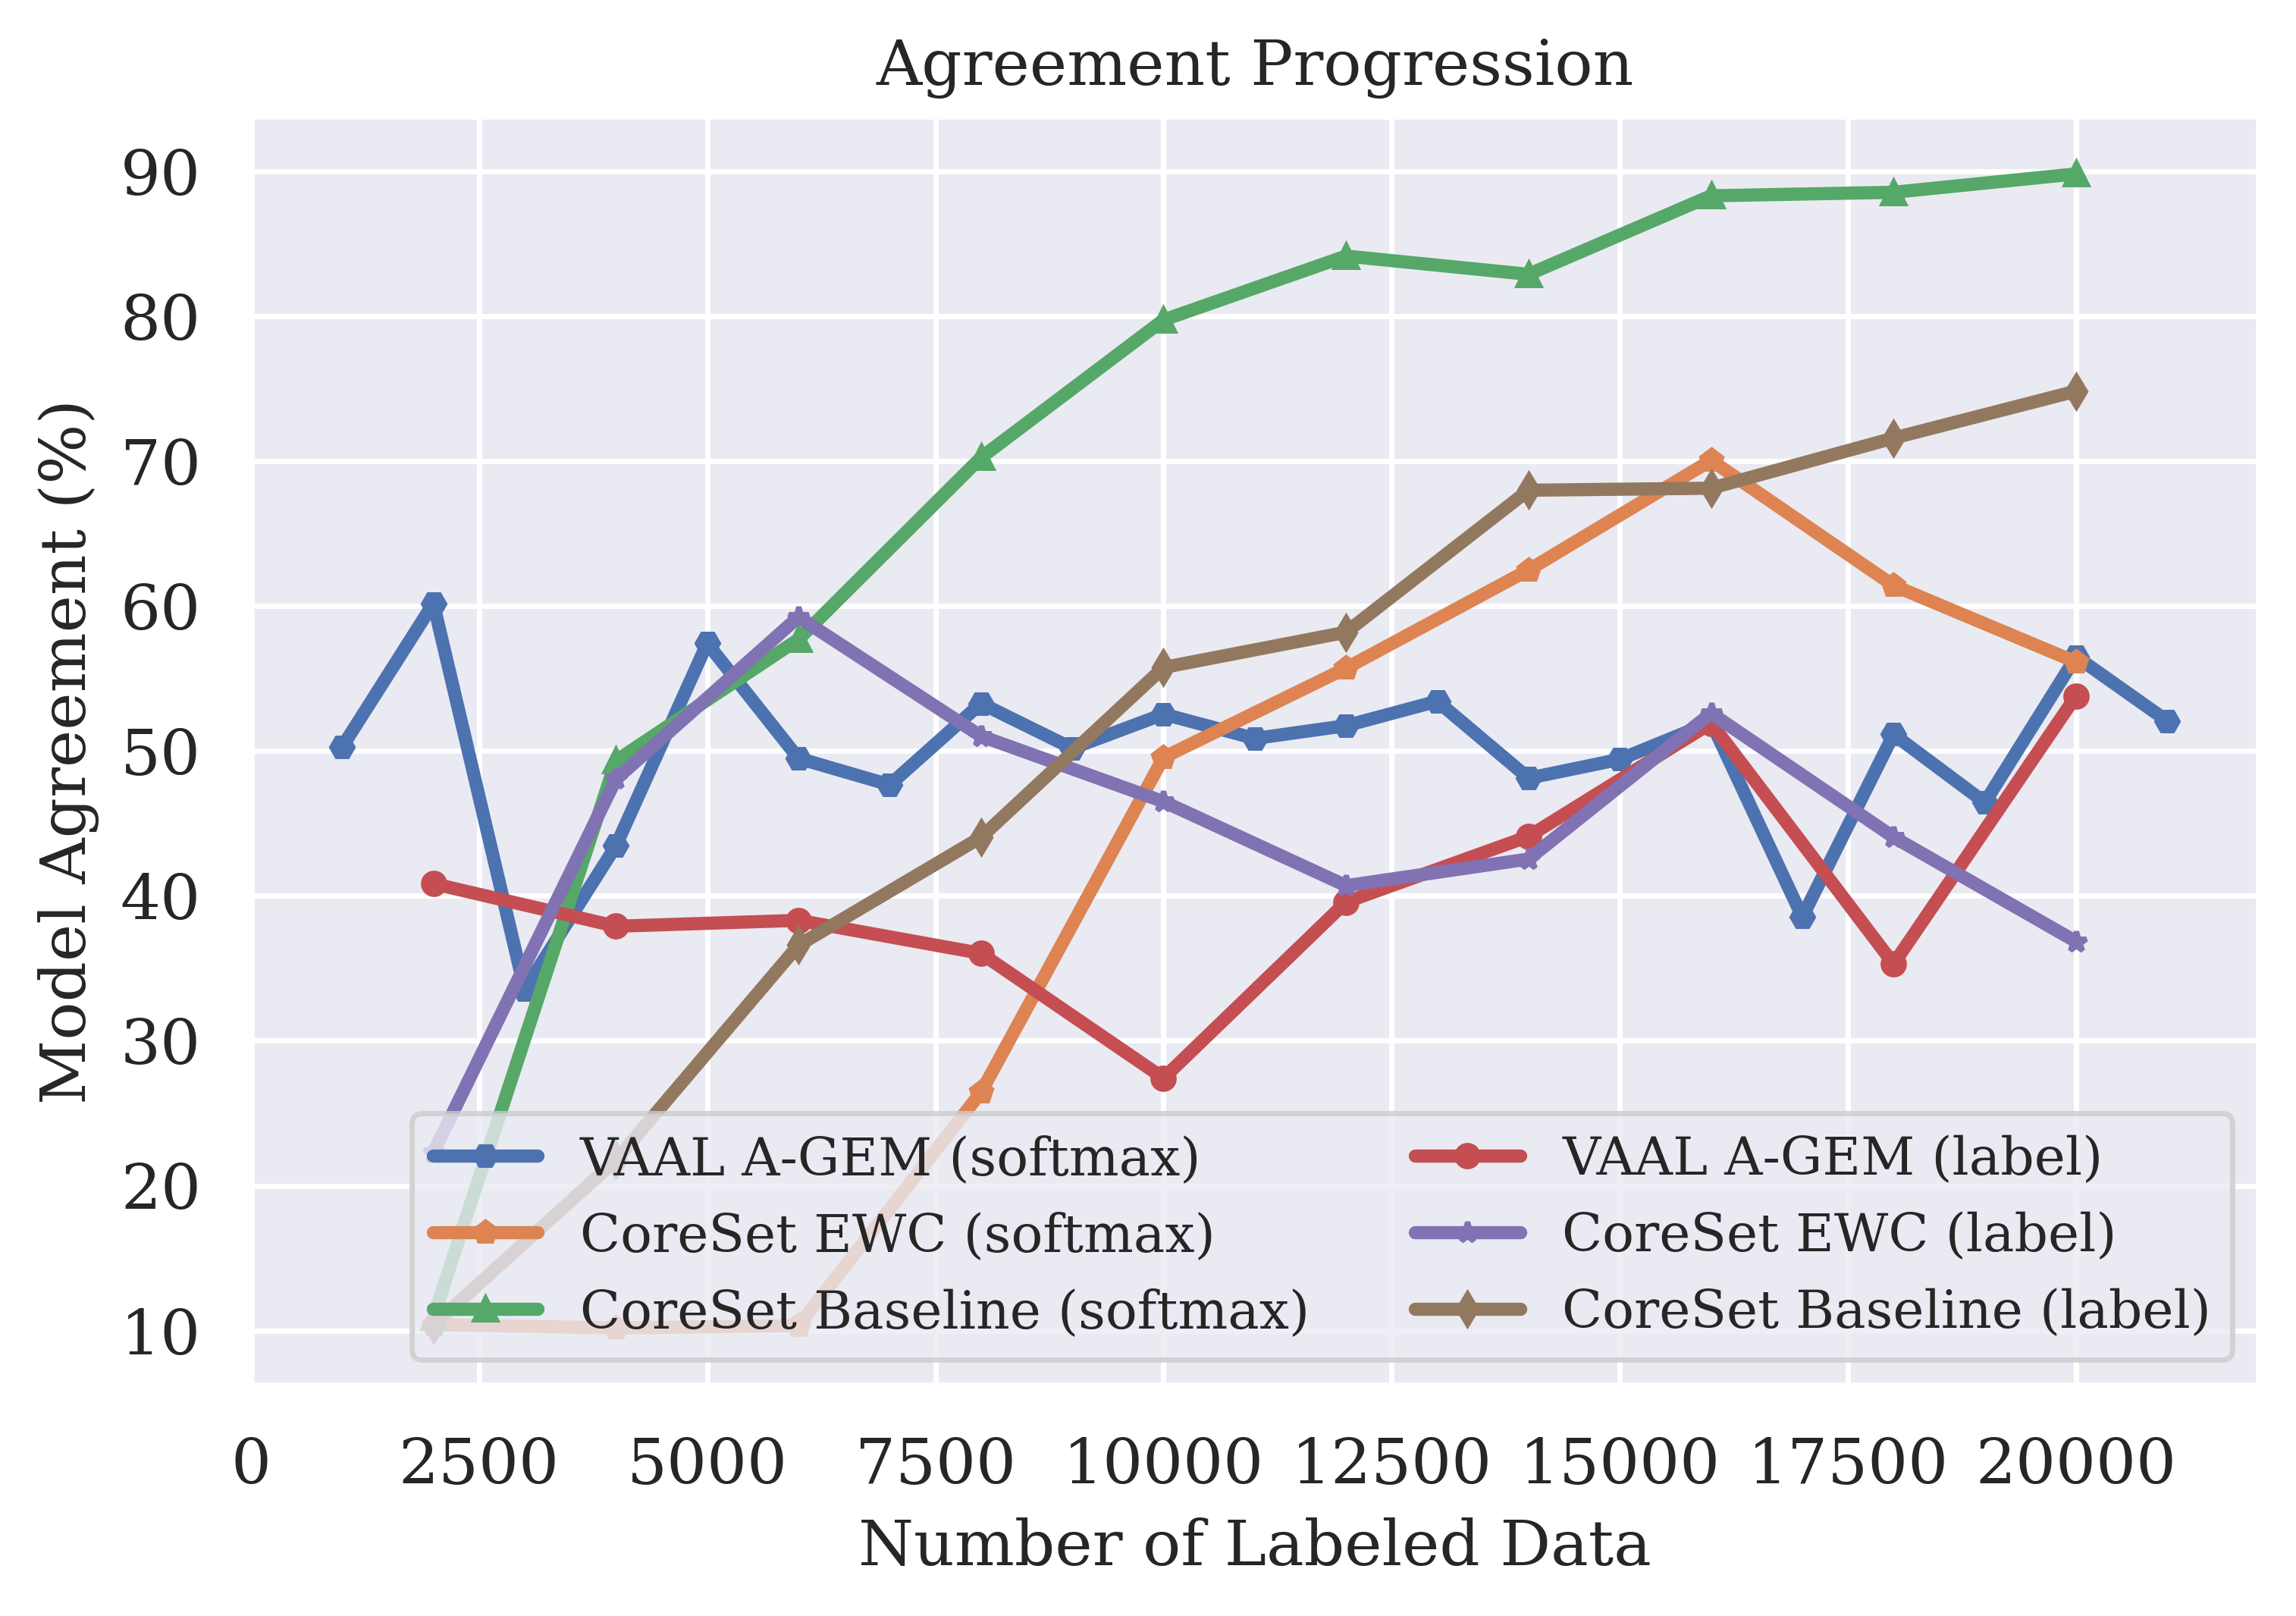
\includegraphics[width=0.5\linewidth]{images/results_CALMS/mnist_vaal_agem.png}
    \caption{Agreement Comparison for Model Stealing on MNIST using \gls{vaal} and \gls{a-gem}}
    \label{fig:CALMSmnistVAAL_AGEM}
\end{figure}

% Todo: Das hier sinnvoll strukturieren
\subsubsection{Evaluation of ActiveThief}
\label{sec:Evaluation:Results:MS:ActiveThief}
Because we build our Continual Active Learning approach upon the ActiveThief framework, we believe that it is important to rigorously evaluate it before we apply Continual Active Learning to it. In the ActiveThief paper \cite{pal2020activethief}, Pal et al. evaluate Active Learning
for Model Stealing for Computer Vision and Natural Language Processing tasks. Since this thesis focuses on Computer Vision tasks, we only investigate the part of the ActiveThief framework that deals with Computer Vision tasks. For the ActiveThief framework, Pal et al. introduce a
proprietary thief dataset, which we dubbed SmallImagenet, and three different target model architectures which we call ActiveThiefConv2, ActiveThiefConv3 and ActiveThiefConv4. In the following we will evaluate the influence of the thief dataset and the target model architecture on
the success of the Model Stealing attack. \par
We start off by computing the validation accuracies of the ActiveThiefConv Model family which both the ActiveThief framework and ours uses as target and substitute models. While these figures have not been given by the authors of ActiveThief in their paper, we believe that they are
important to understand the performance of the ActiveThief framework and of our Continual Active Learning approach. Each model of the ActiveThiefConv family is trained on MNIST and CIFAR-10. Additionally, we train ActiveThiefConv3 on CIFAR-100, because we will conduct experiments
with CIFAR-100 in section \ref{sec:Evaluation:Results:MS:CAL}. We omit the results for ActiveThiefConv2 and ActiveThiefConv4 on CIFAR-100 because they are not relevant to this thesis. The results can be found in table \ref{fig:TargetModelAccuracies}. The results show that the
most complex model ActiveThiefConv4 achieves the highest validation accuracy on both MNIST and CIFAR-10. While the validation accuracy for MNIST is very high for all models, there is a difference in validation accuracy of almost 20 percentage points between ActiveThiefConv2 and
ActiveThiefConv4 on CIFAR-10. This shows that the complexity of the target model architecture has a significant influence on the validation accuracy. \par

\begin{table}[h]
    \centering
    \begin{tabular}{c| c c c} 
        \hline
        \diagbox[width=9em]{Dataset}{Architecture} &  ActiveThiefConv2 & ActiveThiefConv3 & ActiveThiefConv4 \\ 
        \hline 
        MNIST & 98.42\% & 98.91\% & 99.01\% \\
        CIFAR-10 & 66.61\% & 80.67\% & 84.47\% \\
        CIFAR-100 & - & 42.90\% & - \\
        \hline
    \end{tabular}
    \caption[Validation accuracies of our target model architectures]{Validation accuracies of our target model architectures on MNIST,CIFAR-10 and CIFA-100. 
    We omit the results for ActiveThiefConv2 and ActiveThiefConv4 on CIFAR-100 because they are not used in the experiments.}
    \label{fig:TargetModelAccuracies}
\end{table}

Next, we evaluate the influence of the target model architecture and substitute model architecture on the success of the Model Stealing attack. We use the ActiveThiefConv Model family as target and substitute models and perform one model stealing attack for each combination of
target and substitute model. We use the Active Learning strategy CoreSet with a batch size of 1000 and a total budget of 20000 to perform the attacks. The results can be seen in table \ref{fig:ModelStealingNNArchitecturesCIFAR}. The numbers reported in the table represent the 
agreement between the target and substitute model on the validation set of the CIFAR-10 dataset at the end of each experiment. Overall, we observe that the agreement between the target and substitute model is highest when we use a target model of low complexity (i.e. ActiveThiefCon2)
and a substitute model of moderate to high complexity (i.e. ActiveThiefConv3 and ActiveThiefConv4). This is in line with the results of the ActiveThief paper \cite{pal2020activethief}, however we report the accuracy after a budget of 20000, whereas Pal et al. presumably report the
accuracy after training on the full thief dataset. To study the behavior of model stealing attacks using different model architectures further, we conduct the same experiment using MNIST as the target model dataset. The results of this experiment can be found in table 
\ref{fig:ModelStealingNNArchitecturesMNIST}. The results of this experiment are similar to the results of the experiment on CIFAR-10, however it is evident that the discrepancies between the target and substitute model combinations are larger. \par

\begin{table}[h]
    \centering
    \begin{tabular}{c | c c c} 
        \hline
        \diagbox[width=12em]{Substitute Model}{Target Model} &  ActiveThiefConv2 & ActiveThiefConv3 & ActiveThiefConv4 \\ 
        \hline 
        ActiveThiefConv2 & 57.46 & 54.88 & 48.16 \\
        ActiveThiefConv3 & 61.02 & 71.99 & 71.61 \\
        ActiveThiefConv4 & 60.5 & 71.75 & 71.56 \\
        \hline
    \end{tabular}
    \caption[Model agreement of the ActiveThiefConv family on CIFAR-10]{Model agreement different target and substitute models within the ActiveThiefConv Model family on CIFAR-10. We use the Active Learning strategy CoreSet with a batch size of 1000 to perform the attacks.}
    \label{fig:ModelStealingNNArchitecturesCIFAR}
\end{table}


\begin{table}[h]
    \centering
    \begin{tabular}{c | c c c} 
        \hline
        \diagbox[width=12em]{Substitute Model}{Target Model} &  ActiveThiefConv2 & ActiveThiefConv3 & ActiveThiefConv4 \\ 
        \hline 
        ActiveThiefConv2 & 48.65 & 63.16 & 55.95 \\
        ActiveThiefConv3 & 67.71 & 90.65 & 71.16 \\
        ActiveThiefConv4 & 75.38 & 82.56 & 89.40 \\
        \hline
    \end{tabular}
    \caption[Model agreement of the ActiveThiefConv family on MNIST]{Model agreement different target and substitute models within the ActiveThiefConv Model family on MNIST. We use the Active Learning strategy CoreSet with a batch size of 1000 to perform the attacks.}
    \label{fig:ModelStealingNNArchitecturesMNIST}
\end{table}

After evaluating the influence of the target and substitute model architecture on the success of the model stealing attack, we now evaluate how the thief dataset effects Model Stealing Attacks. Our motivation for this experiment is that Pal et al. 
mention having tested CIFAR-10 as a thief dataset with without success. We perform a model stealing attack using ActiveThiefConv3 as the target and substitute model and CoreSet with batch size 2000 as our Active Learning strategy. The total query budget
is 20000. We used MNIST as the target model dataset and change between Small ImageNet, Tiny ImageNet and CIFAR-10 as our thief datasets. The results of this experiment can be seen in figure \ref{fig:Evaluation:Results:CAL:EffectDataset}. While the model agreement 
increases throughout the experiment when using Small ImageNet, the model agreement for Tiny ImageNet plateaus after just 3 iterations at 20\%. Model Stealing with CIFAR-10 yields the best results, however. At the end of the experiment, the setup with CIFAR-10 as 
the thief dataset achieves a Model Agreement which is 5 percentage points higher than the setup with Small Imagenet as the thief dataset. \par

\begin{figure}[h]
    \centering
    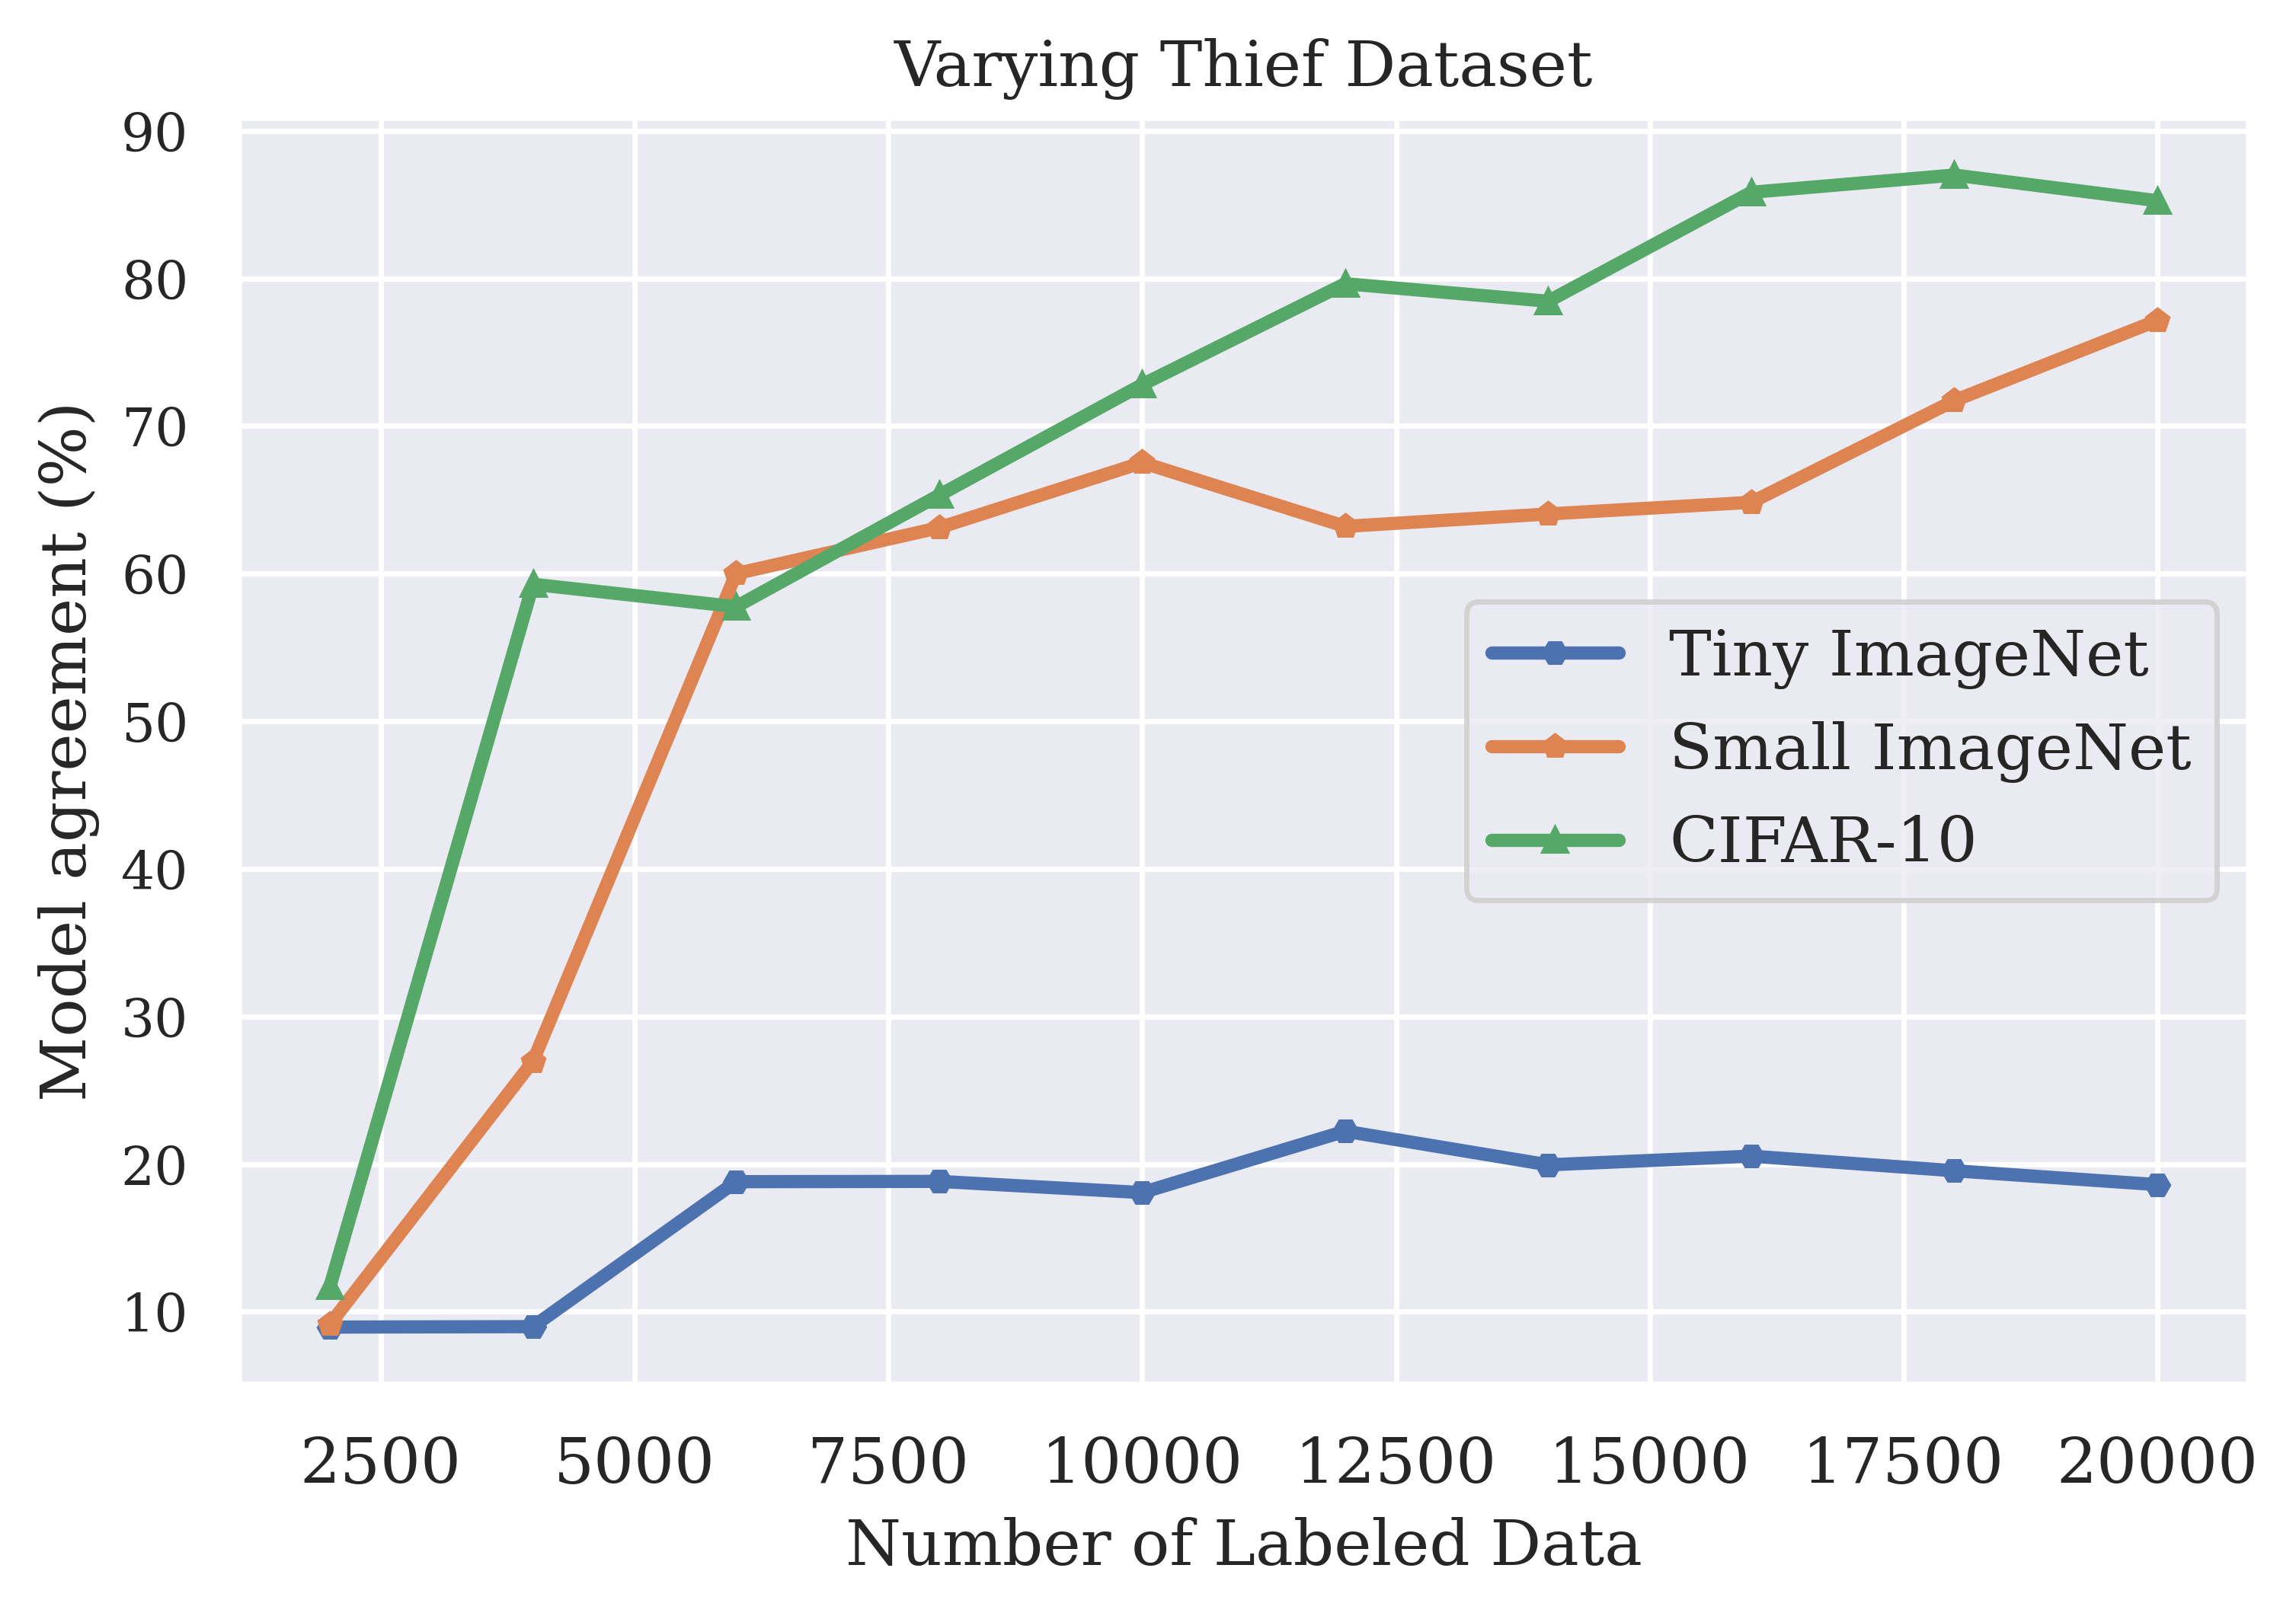
\includegraphics[width=0.8\linewidth]{images/results_CALMS/effect_dataset.png}
    \caption[Effect of Thief Dataset choice on the success of Model Stealing Attacks]{Comparison of Model Agreement when performing a model stealing attack using the datasets Tiny Imagenet, Small ImageNet and CIFAR-10. We perform Active Learning using the 
    straegy CoreSet with a batch size of 2000 for the experiments. The target model dataset used is MNIST.s}
    \label{fig:Evaluation:Results:CAL:EffectDataset}
\end{figure}